% Some kind of 35t analysis -- looking at pi0s in 35t
% Target: 30 pages

\graphicspath{{35tonAnalysis/Figs/}}

%----------------------------------------------------------------------------------------------------------------------------------------------------------------------------
\chapter{Analysis of 35-ton Data}\label{chap:35tonAnalysis}

The 35-ton run, discussed in Section~\ref{sec:35tonPhaseII}, provided 22 days of good quality (high purity, stable field ($250$~V/cm), stable DAQ), analysable data.  Due to the issues encountered, high quality physics analyses proved very challenging and instead studies, particularly those presented here, focused on trying to understand the detector and characterise previously untested responses.  In this respect, the 35-ton proves to be a vital experiment in informing the next generation of prototypes and even the final DUNE far detector design.  It also boasts unique datasets which no other planned experiment will possess before the full DUNE modules; it is therefore essential as much information as possible is extracted from the 35-ton analyses.

Before analyses are presented, techniques developed to enhance the quality of the data, and the data selection, will be discussed in Section~\ref{sec:Preparing35tonData}.  The main studies, concerning tracks passing across APA gaps and through the APA frames, are presented in Section~\ref{sec:APAGapCrossing} and Section~\ref{sec:APACrossing} respectively before a brief investigation into the performance of basic shower and calorimetric reconstruction on the 35-ton data is discussed in Section~\ref{sec:ShowerData}.  A summary is provided in Section~\ref{sec:35tonDataSummary}.

%----------------------------------------------------------------------------------------------------------------------------------------------------------------------------
\section{Preparing 35-ton Data for Analysis}\label{sec:Preparing35tonData}

To ensure analyses are as accurate as possible, careful preselection and preprocessing of the data is performed.  Methods for producing the analysable sample are discussed in this section.

%----------------------------------------------------------------------------------------------------------------------------------------------------------------------------
\subsection{Selecting the Data}\label{sec:SelectingTheData}

The level of noise present in the TPC data varied significantly between runs and is immediately evident when analysing the RMS of the charge read out on a particular channel.  Figure~\ref{fig:DataRMS} shows a comparison of this metric for `good' and `bad' runs.  In this case, the figures show a `normal noise' run and one taken with the detector in the `high noise' state.  The noise worsened as the experiment progressed but, in general, runs taken with normal noise and most of the TPC operating during the period of stable data-taking were used to assemble a `good run' list by the collaboration.

\begin{figure}
  \centering
  \begin{subfigure}{0.45\linewidth}
    \centering
    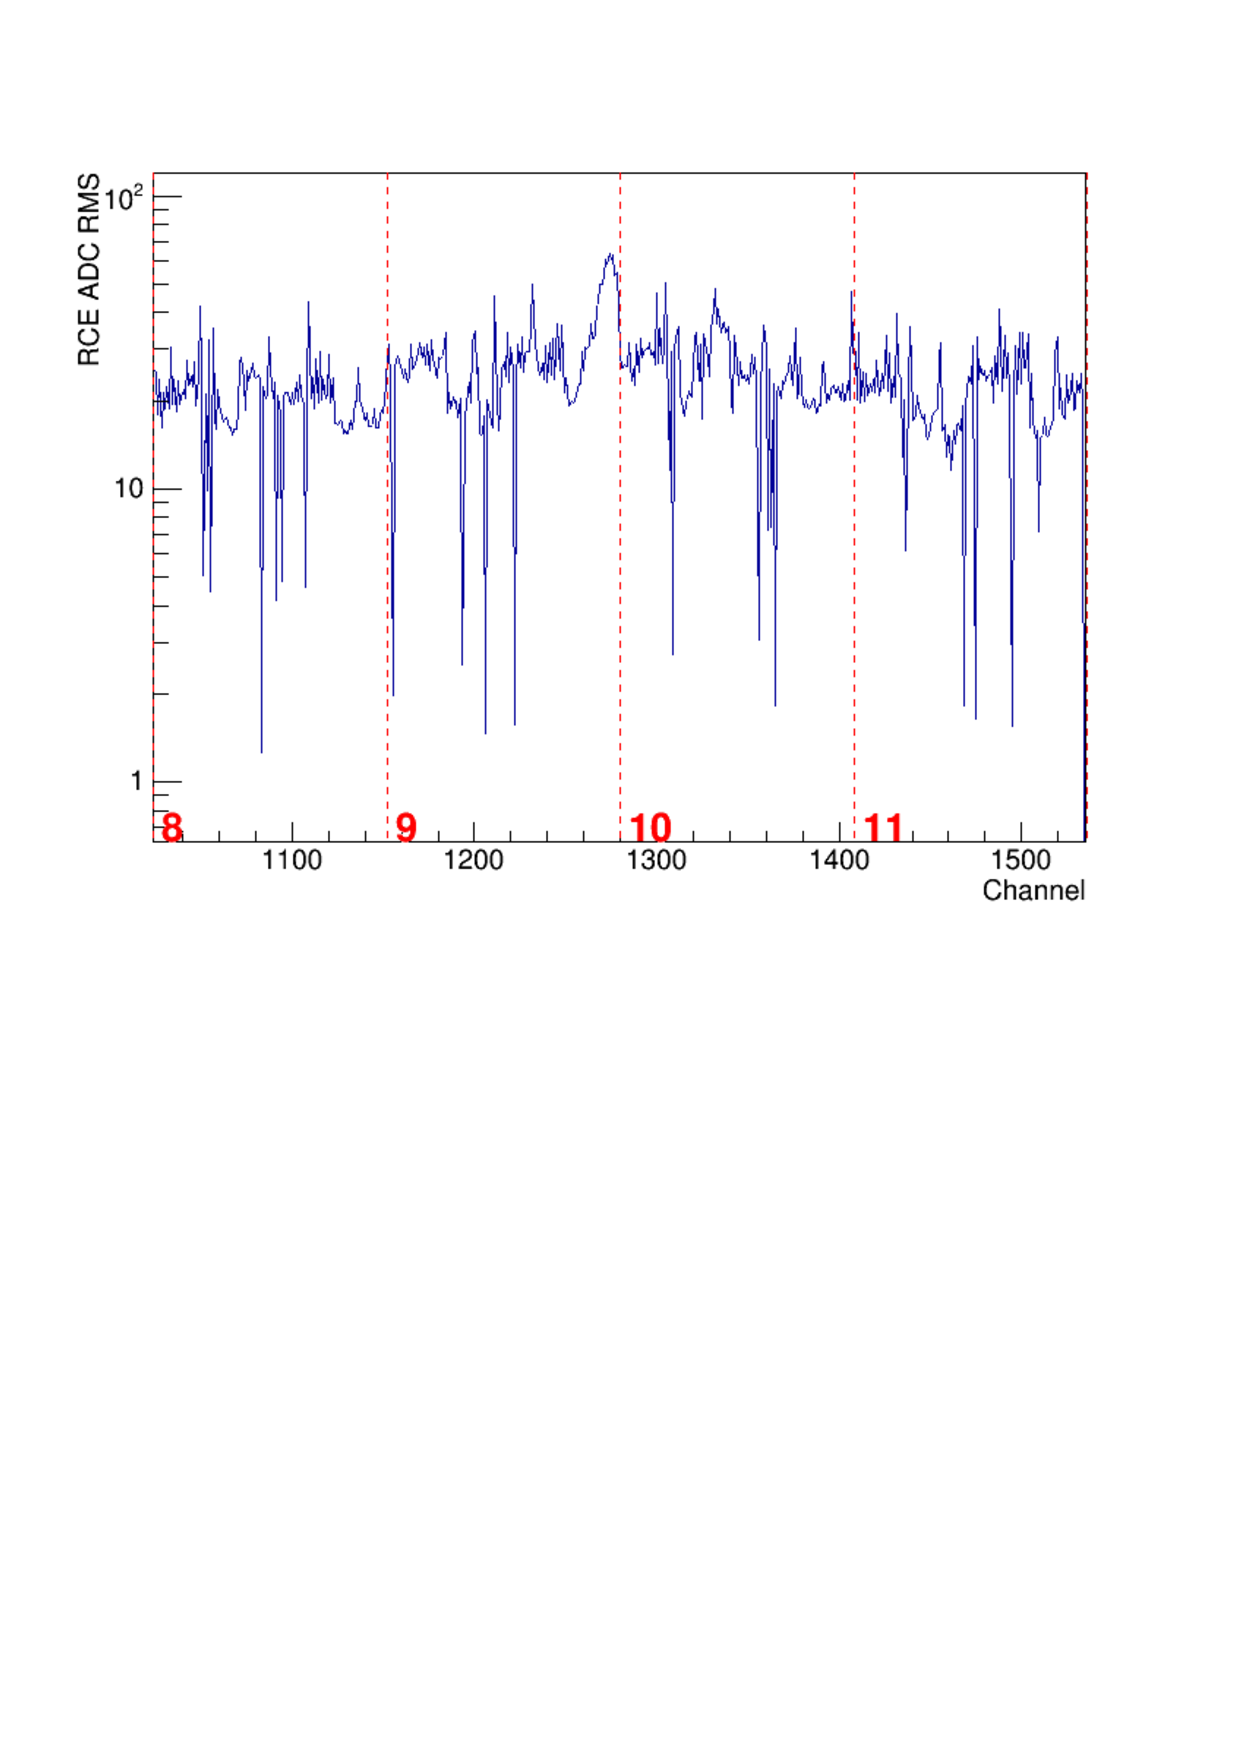
\includegraphics[width=0.95\textwidth]{DataRMSGood.pdf}
    \caption{Good run.}
    \label{fig:DataRMSGoodRun}
  \end{subfigure}
  \hfill
  \begin{subfigure}{0.45\linewidth}
    \centering
    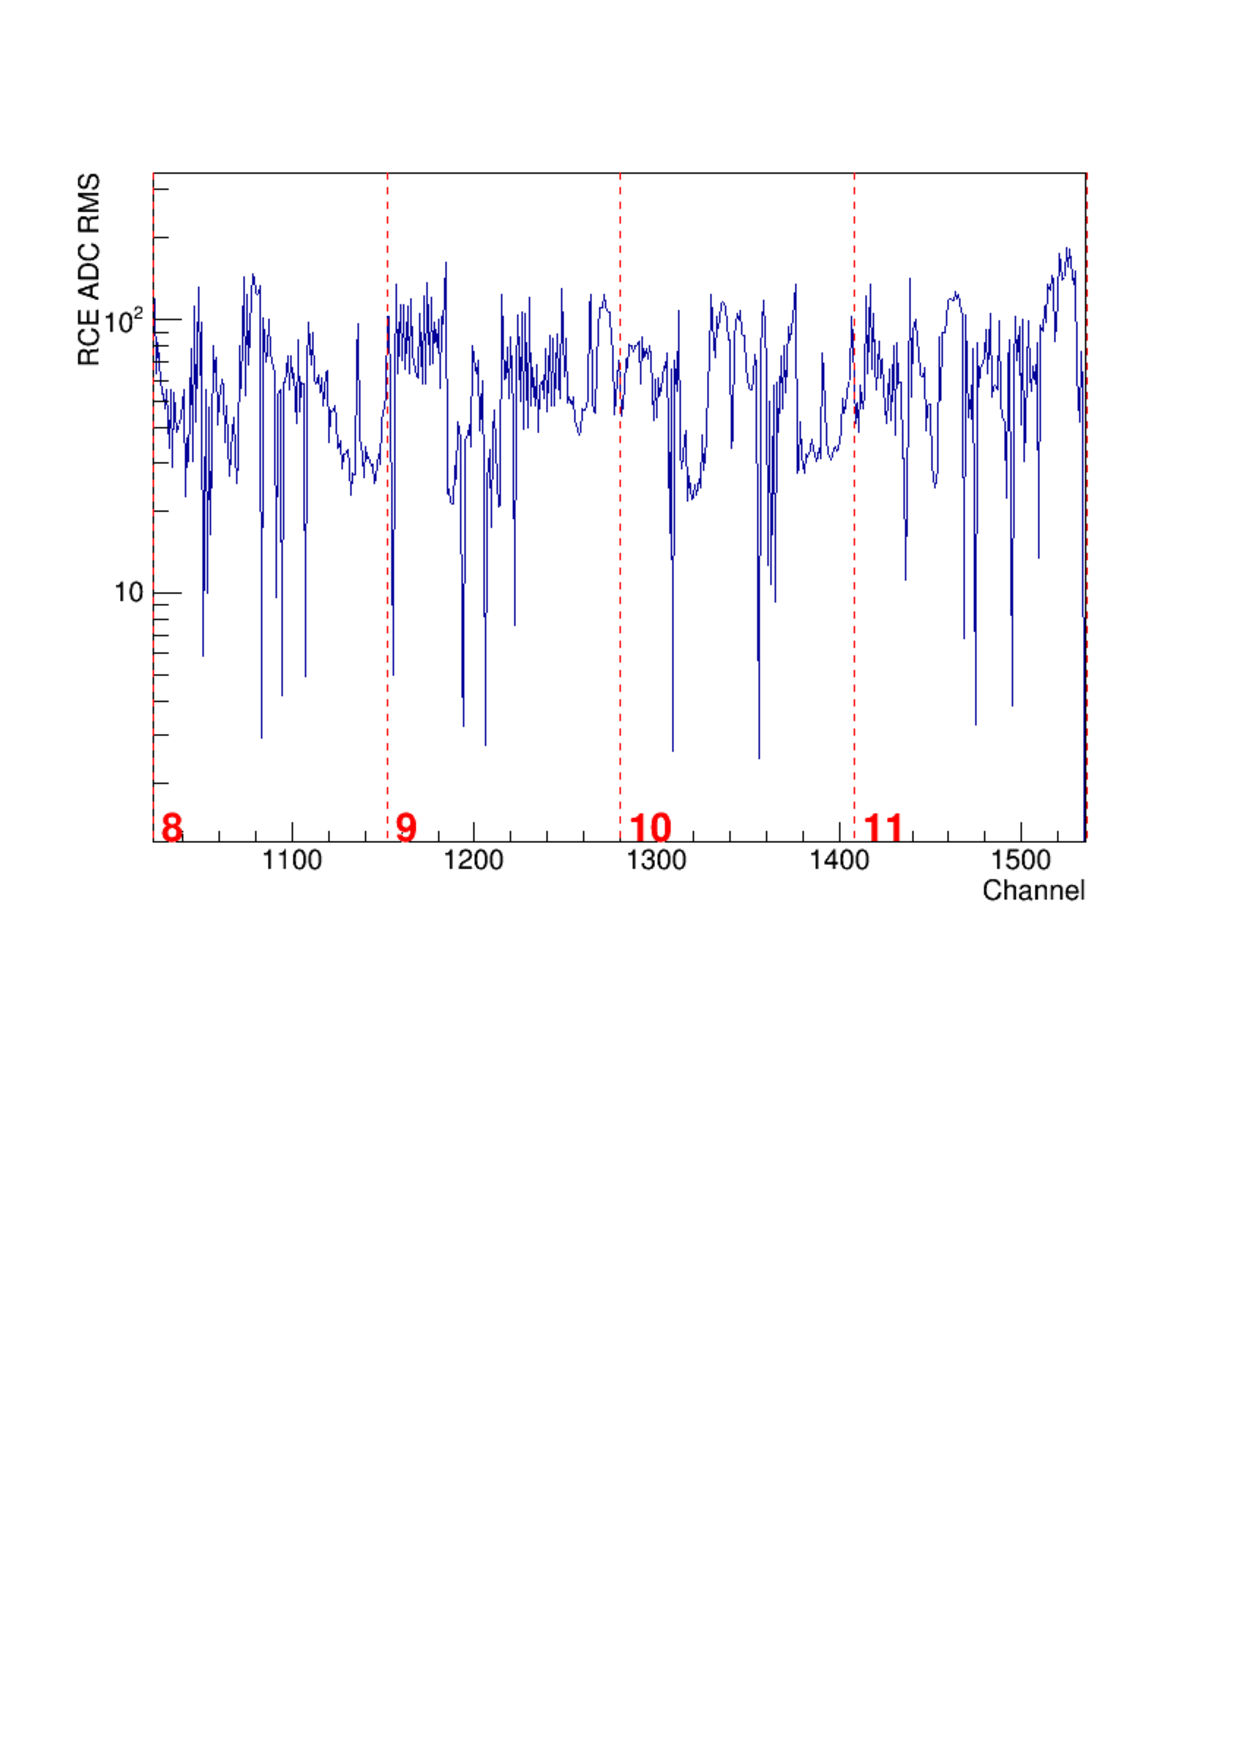
\includegraphics[width=0.95\textwidth]{DataRMSBad.pdf}
    \caption{Bad run.}
    \label{fig:DataRMSBadRun}
  \end{subfigure}
  \caption[Comparison between noise levels for `good' and `bad' 35-ton runs.]{Comparison between noise levels for `good' and `bad' 35-ton runs.  The channels shown are on APA2 (online convention, APA0 offline) and are read out by RCEs 8 through 11 (labelled).  The increase in read out charge RMS is evident in the case of the noisy run.  These plots are from runs 15797 (Fig \ref{fig:DataRMSGoodRun}) and 15790 (Figure~\ref{fig:DataRMSBadRun}) and were taken only 50 minutes apart.}
  \label{fig:DataRMS}
\end{figure}

In all there were 1269 runs used for analysis, containing some data taken before the FNAL site wide power outage (3rd March 2016) with most the week after stabilising the experiment again (9th March -- 17th March 2016), and representing around 80\% of all runs from the period.  A selection of bad channels, classified as either `dead' (electrically) or `bad' (exhibit sufficiently more than average noise), constitute 13--25\% of the total number of channels \cite{Kirby2016}.

Due to the continuous nature of data taking, there is a non-trivial correlation between a `DAQ event', a collection of fragments read out by the DAQ, and a `physics event', an event in which particle interactions occurred.  The external triggers used in the 35-ton, namely the external muon scintillators and the photon detectors, are used to define the event time.  Given the trigger rate at which most data was taken ($\sim1$~Hz), a typical run comprising a few thousand events will only contain $\mathcal{O}(10)$ triggered events.  Furthermore, as described in Section~\ref{sec:35tonDataFormats}, these events often straddle multiple DAQ events (previously demonstrated in Figure~\ref{fig:35tonTriggeredEvent}), requiring the use of a splitter/stitcher module to search for triggers within runs and construct physics events containing the information useful for analysis.

%----------------------------------------------------------------------------------------------------------------------------------------------------------------------------
\subsection{Improving Data Quality}\label{sec:ImprovingDataQuality}

Two issues present in the raw data, namely the presence of correlated noise and the stuck codes in the digitiser (both described in Section~\ref{sec:35tonPhaseIIOutcomesCryostatTPC}), are dealt with as an initial step of the reconstruction.  Initially, an algorithm attempts to correct for the stuck bits analyses waveforms on a wire and identifies problematic ADCs; interpolating between charges read out at neighbouring times is successful at reconstructing the initial waveform in most cases.  Figure~\ref{fig:StuckBitInterpolation} demonstrates this interpolation method on simulated data.  The effect of applying this algorithm on a full waveform, to correct for all the stuck bits, is apparent in Figure~\ref{fig:StuckBitWaveform}.

\begin{figure}
  \centering
  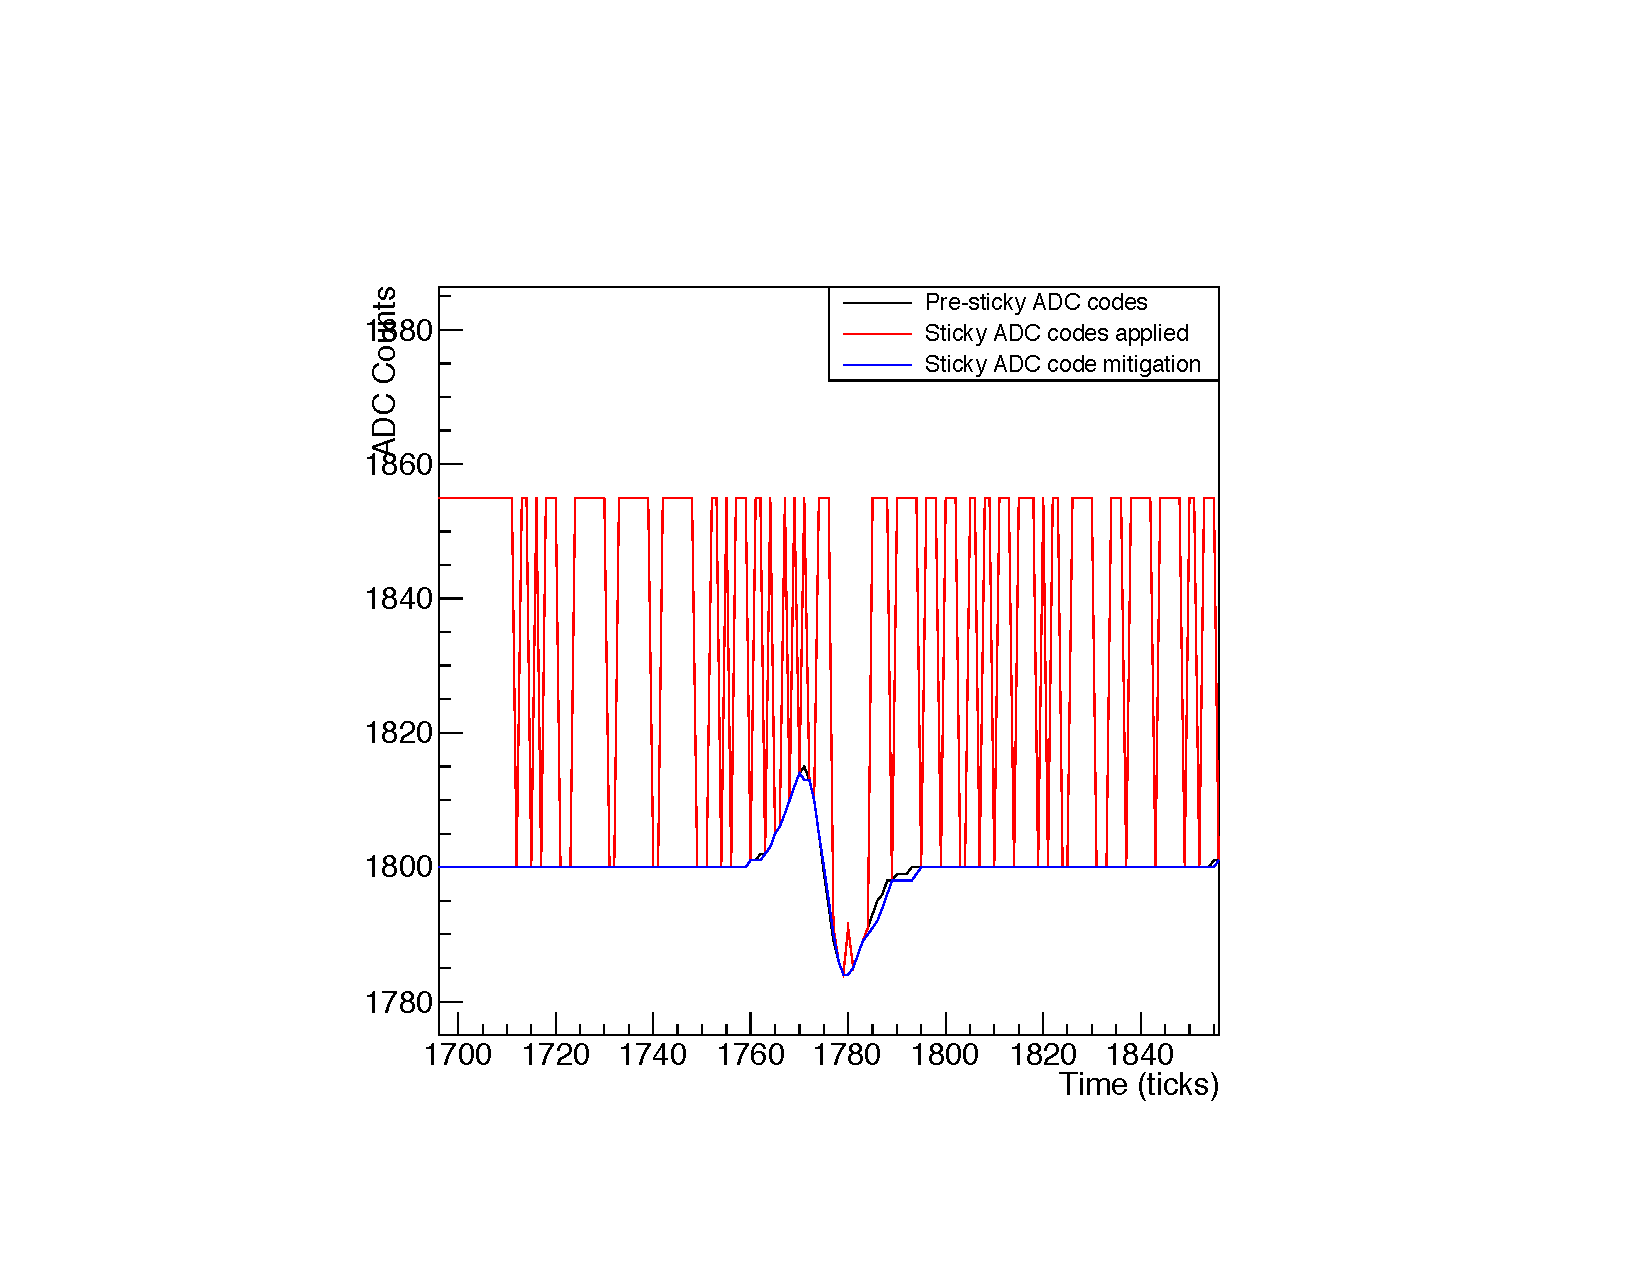
\includegraphics[width=8cm]{stuckbitsremoval.pdf}
  \caption[Simulated demonstration of the method used to correct for stuck codes in the 35-ton data.]{Simulated demonstration of the method used to correct for stuck codes in the 35-ton data \cite{Insler2016}.  On a given channel, ADCs exhibiting the consequences of this problem are corrected by interpolating charge at neighbouring time units.  This is tested by simulating a waveform and applying the observed stuck code effect, demonstrated by the black and red waveforms respectively.  The efficacy of the developed algorithm at correcting the afflicted bits may then be evaluated, shown by the blue trace.}
  \label{fig:StuckBitInterpolation}
\end{figure}

\begin{figure}
  \centering
  \begin{subfigure}[t]{0.48\linewidth}
    \centering
    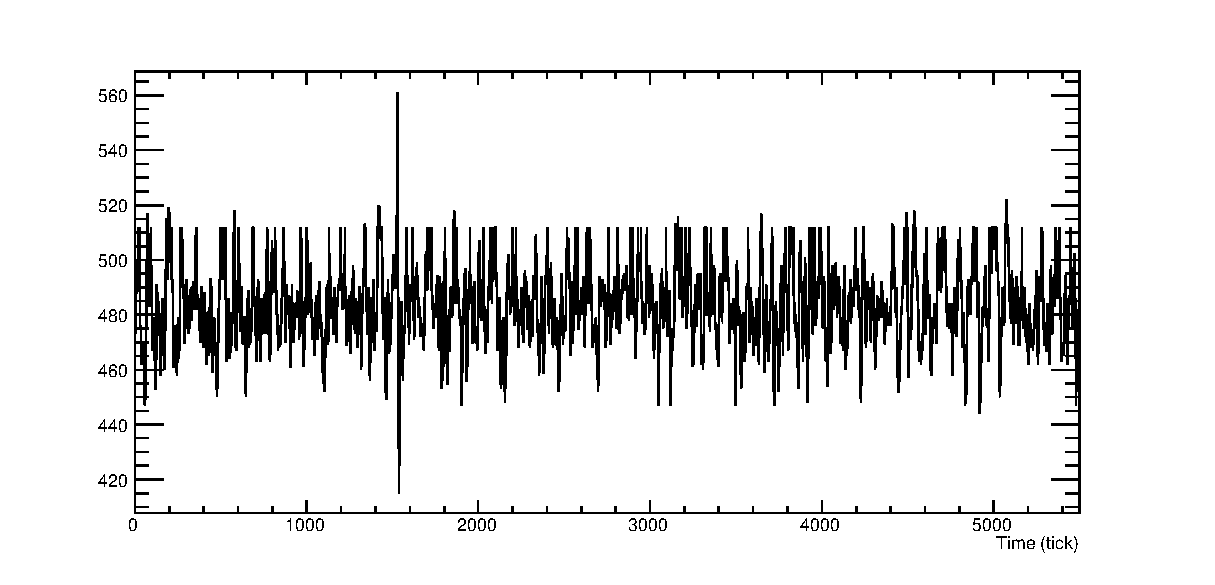
\includegraphics[width=\textwidth]{raw_stuck.eps}
    \caption{Raw waveform before correcting for stuck bits.}
    \label{fig:StuckBitWaveformStuck}
  \end{subfigure}
  \hfill
  \begin{subfigure}[t]{0.48\linewidth}
    \centering
    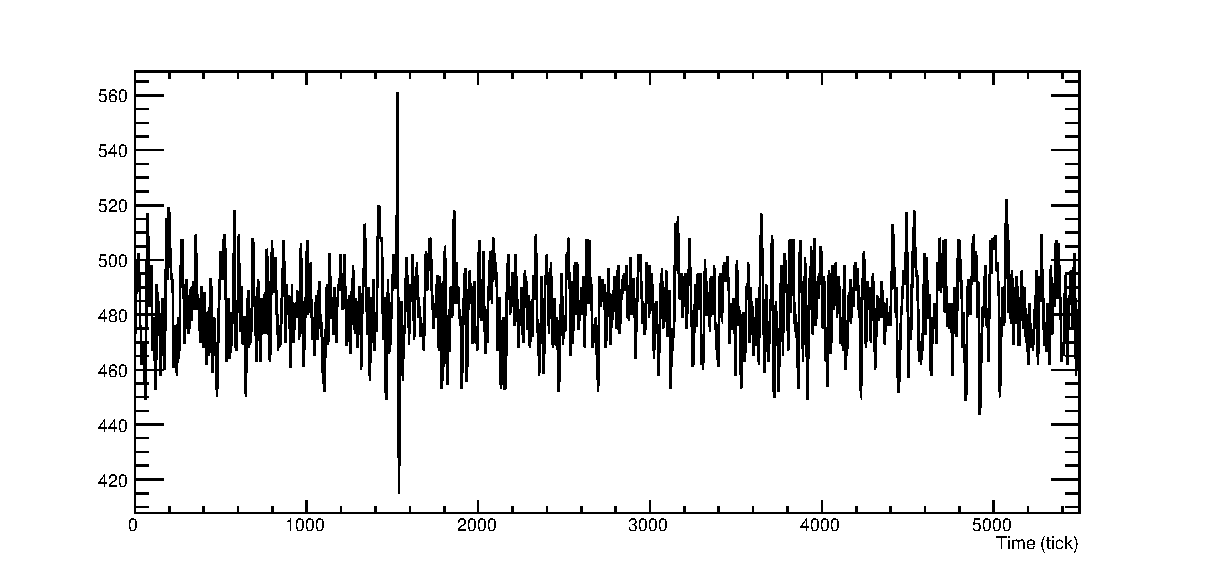
\includegraphics[width=\textwidth]{raw_unstuck.eps}
    \caption{After applying stuck bit mitigation.}
    \label{fig:StuckBitWaveformUnstuck}
  \end{subfigure}
  \caption[The effect of applying stuck bit mitigation to a waveform as seen in raw 35-ton data.]{The effect of applying stuck bit mitigation to a waveform as seen in raw 35-ton data.  This particular waveform is from run 15660, channel 722 (induction channel).}
  \label{fig:StuckBitWaveform}
\end{figure}

Following this process, a coherent noise removal stage is applied.  This simply looks at the average noise across channels sharing a front-end voltage regulator and removes this component from the readout ADC for each channel.  The effect of this correction is seen in Figure~\ref{fig:CoherentNoiseRemoval}.

\begin{figure}
  \centering
  \begin{subfigure}[t]{0.48\linewidth}
    \centering
    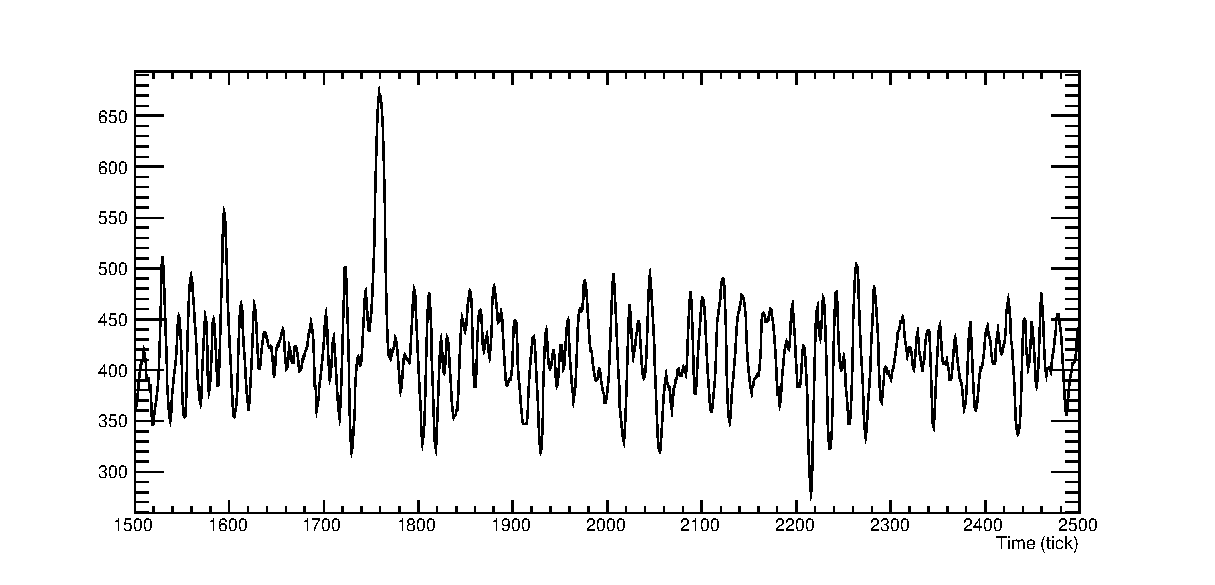
\includegraphics[width=\textwidth]{raw_noise.eps}
    \caption{Waveform before removing coherent noise.}
    \label{fig:CoherentNoiseRemovalNoise}
  \end{subfigure}
  \hfill
  \begin{subfigure}[t]{0.48\linewidth}
    \centering
    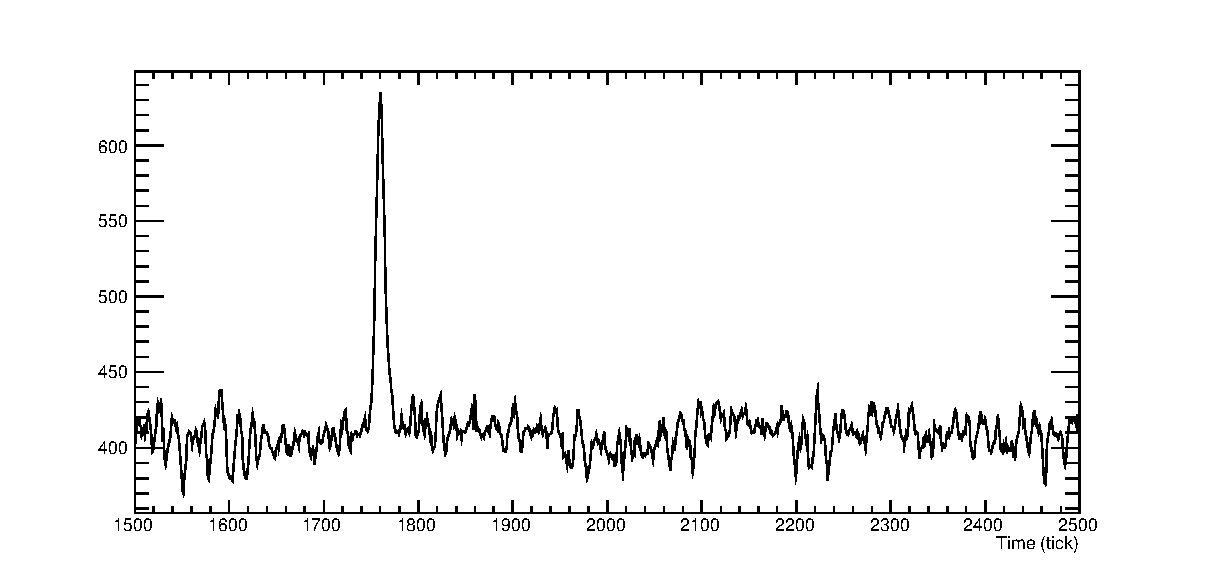
\includegraphics[width=\textwidth]{raw_nonoise.eps}
    \caption{After removing coherent noise.}
    \label{fig:CoherentNoiseRemovalNoNoise}
  \end{subfigure}
  \caption[The effect of removing coherent noise from all channels on a voltage regulator in the 35-ton data.]{The effect of removing coherent noise from all channels on a voltage regulator in the 35-ton data.  This waveform is from run 15660, channel 2010 (collection channel).  As a result of this process the noise (RMS of ADC values) decreases from 37.1 to 18.8 leaving a signal which is noticeably larger, considerably improving reconstruction performance.}
  \label{fig:CoherentNoiseRemoval}
\end{figure}

%----------------------------------------------------------------------------------------------------------------------------------------------------------------------------
\subsection{Reconstructing Muon Tracks}\label{sec:ReconstructingMuonTracks}

All analyses discussed below only make use of information recorded on the collection planes.  Since the induction wires are longer (a necessity for wrapping), a larger capacitance results in higher noise levels, complicating the reconstruction.  In general, after applying the refinements outlined in Section~\ref{sec:ImprovingDataQuality}, the signals on the collection channels are prominent enough for competent analyses.  The methods used to select tracks are described in this section and applied during the subsequent studies.

Using only the collection plane presents challenges, the most obvious being the impossibility of full 3D reconstruction.  A hit on a collection wire at a given time gives well-defined $x$ and $z$ coordinates but cannot give any information in the $y$-direction.  `Quasi-3D' reconstruction is achieved by making use of the external counters.  Through-going muons are triggered by the coincidence of hits in two opposite counters; this information can be used to give a crude handle on the $y$ position of hits.

Figure~\ref{fig:TrackSelection} outlines the stages of selecting hits originating from the particle track which caused the trigger.  Figure~\ref{fig:TrackSelectionBefore} shows all hits from an example event containing a through-going muon.  The first stage of track selection involves taking those hits which lie in the `counter shadow', the narrow section of the collection plane area physically in between the opposing counters through which the triggering particle passed.  The hits which remain are shown in Figure~\ref{fig:TrackSelectionCounterShadow}.  The track hits are visible along with further, unrelated hits.  These are removed by requiring that only hits on wires with single occupancy be kept, and then applying a linear fit and removing all hits with residual $>2$~cm.  The final output after these stages is shown in Figure~\ref{fig:TrackSelectionFinal}.

\begin{figure}
  \centering
  \begin{subfigure}[t]{0.48\linewidth}
    \centering
    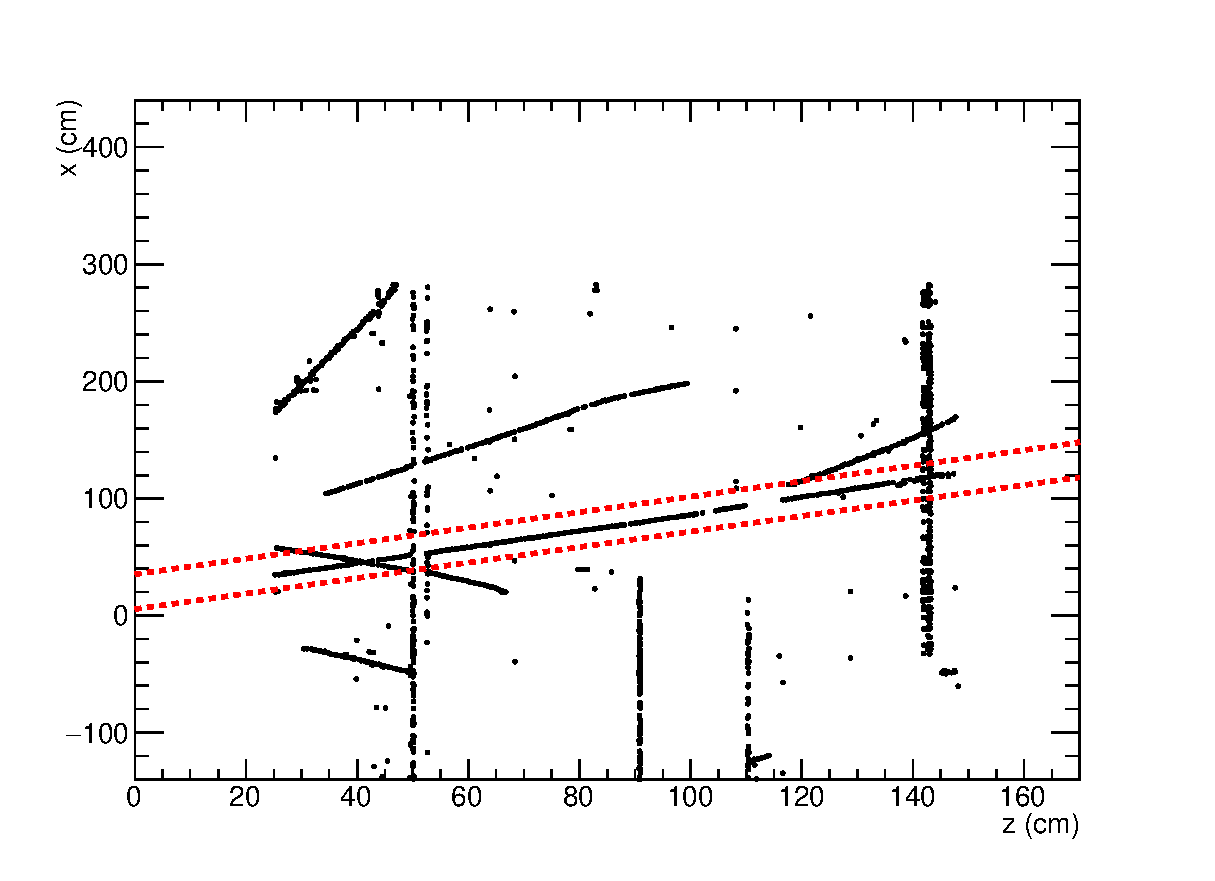
\includegraphics[width=\textwidth]{hitselection_all.eps}
    \caption{All hits before any track selection.  The red lines represent the boundary defined by the edges of the two counters causing the trigger.}
    \label{fig:TrackSelectionBefore}
  \end{subfigure}
  \hfill
  \begin{subfigure}[t]{0.48\linewidth}
    \centering
    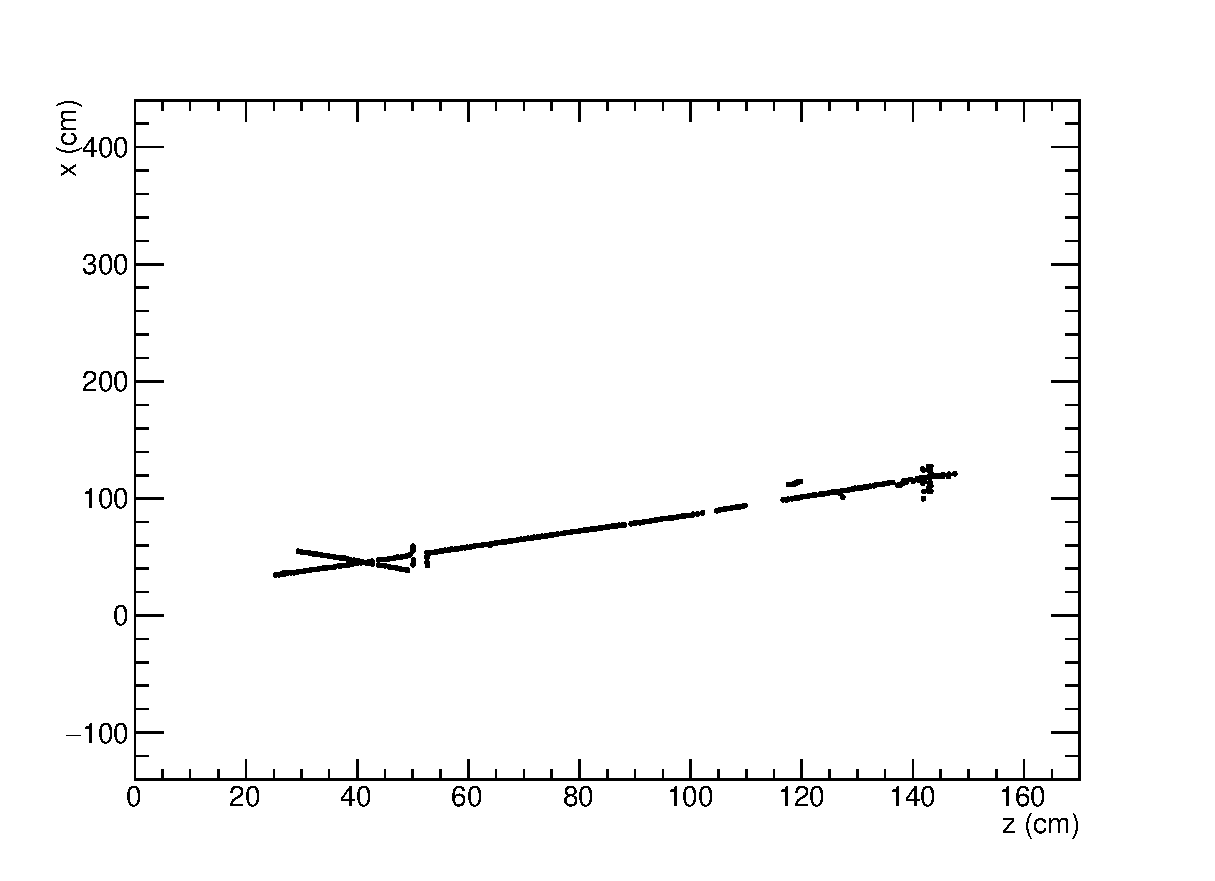
\includegraphics[width=\textwidth]{hitselection_shadow.eps}
    \caption{Hits in the counter shadow.}
    \label{fig:TrackSelectionCounterShadow}
  \end{subfigure}
  \hfill
  \begin{subfigure}[t]{0.48\linewidth}
    \centering
    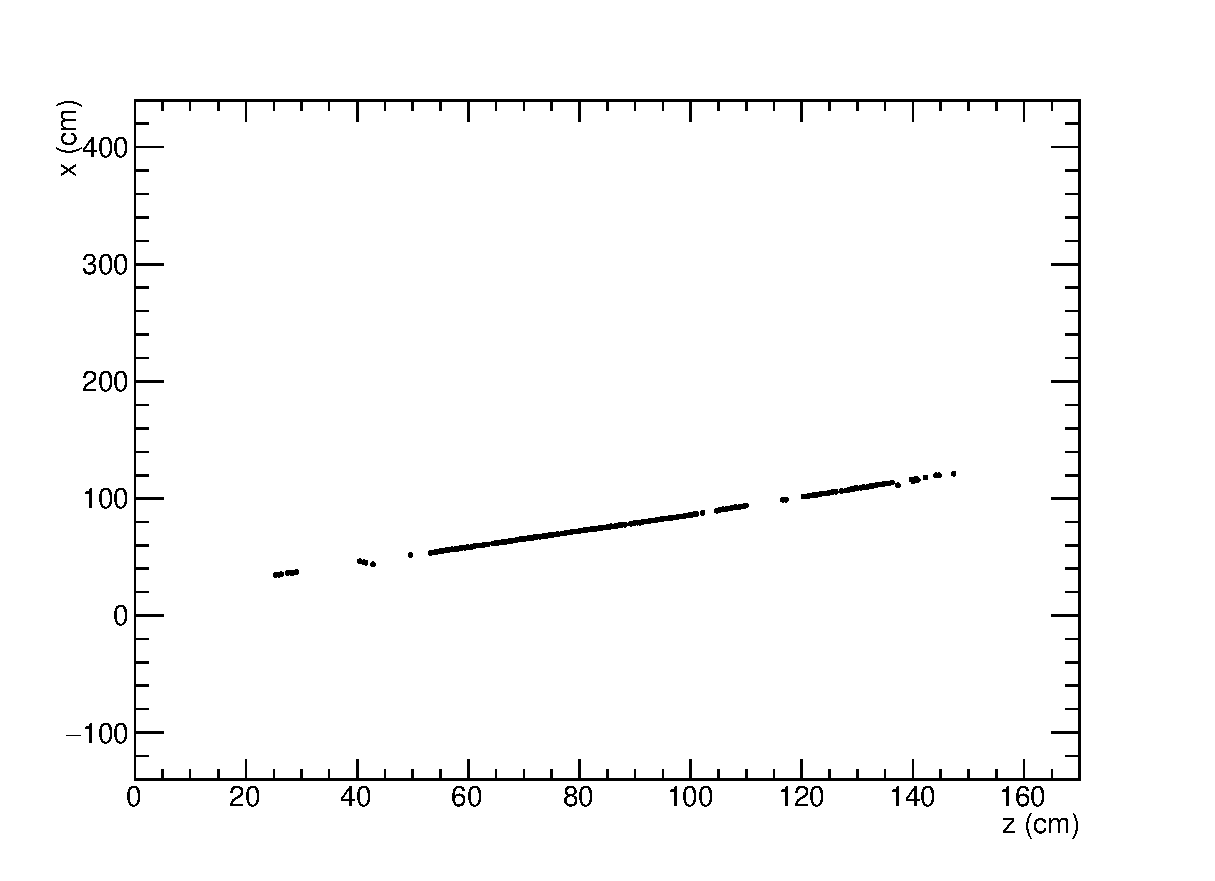
\includegraphics[width=\textwidth]{hitselection_final.eps}
    \caption{Hits on single wire occupancy and with residual $<2$~cm.}
    \label{fig:TrackSelectionFinal}
  \end{subfigure}
  \caption[Demonstration of the successive stages applied to hits on collection wires in the 35-ton data in order to select hits from the through-going track associated with the particle which caused the trigger.]{Demonstration of the successive stages applied to hits on collection wires in the 35-ton data in order to select hits from the through-going track associated with the particle which caused the trigger.  The hits left after all stages are taken forward into the analyses.}
  \label{fig:TrackSelection}
\end{figure}

The result of this track selection, as evident from Figure~\ref{fig:TrackSelectionFinal}, is a well-formed, high quality track with which it is possible to perform analyses.  These will be the focus of the remainder of this chapter.

%----------------------------------------------------------------------------------------------------------------------------------------------------------------------------
\subsection{Preparing Simulated Data}\label{sec:SimulatedData}

Comparisons with simulated data are often essential in understanding various phenomena in the data.  Throughout the analyses presented in this chapter, simulations were used to aid investigations and therefore it is important to ensure the Monte Carlo is as similar to the real data as possible.

The standard LArSoft simulation tools were used as described in Section~\ref{sec:LArSoft}, employing the CRY cosmic ray generator \cite{CRY2007}.  The data passing through the detector were filtered on counter coincidences, exactly as the raw data is triggered.  The simulated data was then processed in the same way as the real data and reconstructed using the methods described in Section~\ref{sec:ReconstructingMuonTracks}.

%% %----------------------------------------------------------------------------------------------------------------------------------------------------------------------------
%% \section{LAr Purity from Crossing Muons}\label{sec:PurityAnalysis}

%% {color{red} Lee: As we have previously discussed, I'm happy to get rid of this section is we don't think it's worth it!}

%% The purity of the liquid argon is directly related to the concentration of electronegative impurities present in the medium which may capture drift electrons before they reach the anode planes.  This gives rise to the concept of `electron lifetime', $\tau$, which affects the charge $Q_{\textnormal{c}}$ collected by the readout wires;
%% \begin{equation}\label{eq:ElectronLifetime}
%% Q_{\textnormal{c}} = (Q_{\textnormal{i}} - Q_{\textnormal{r}}) e^{-t/\tau},
%% \end{equation}
%% where $Q_{\textnormal{i}}$ is the ionised charge, $Q_{\textnormal{r}}$ is the charge lost due to initial recombination with the position ion and $t$ is the drift time of the charge packet.

%% It is possible to make a measurement of the electron lifetime directly from crossing muon tracks and this will be briefly described in this section.  The analysis here serves mainly to demonstrate how these measurements are made and to produce preliminary results; a rigorous assessment is a in-depth study in itself and is not attempted in this thesis.

%% \begin{figure}
%%   \centering
%%   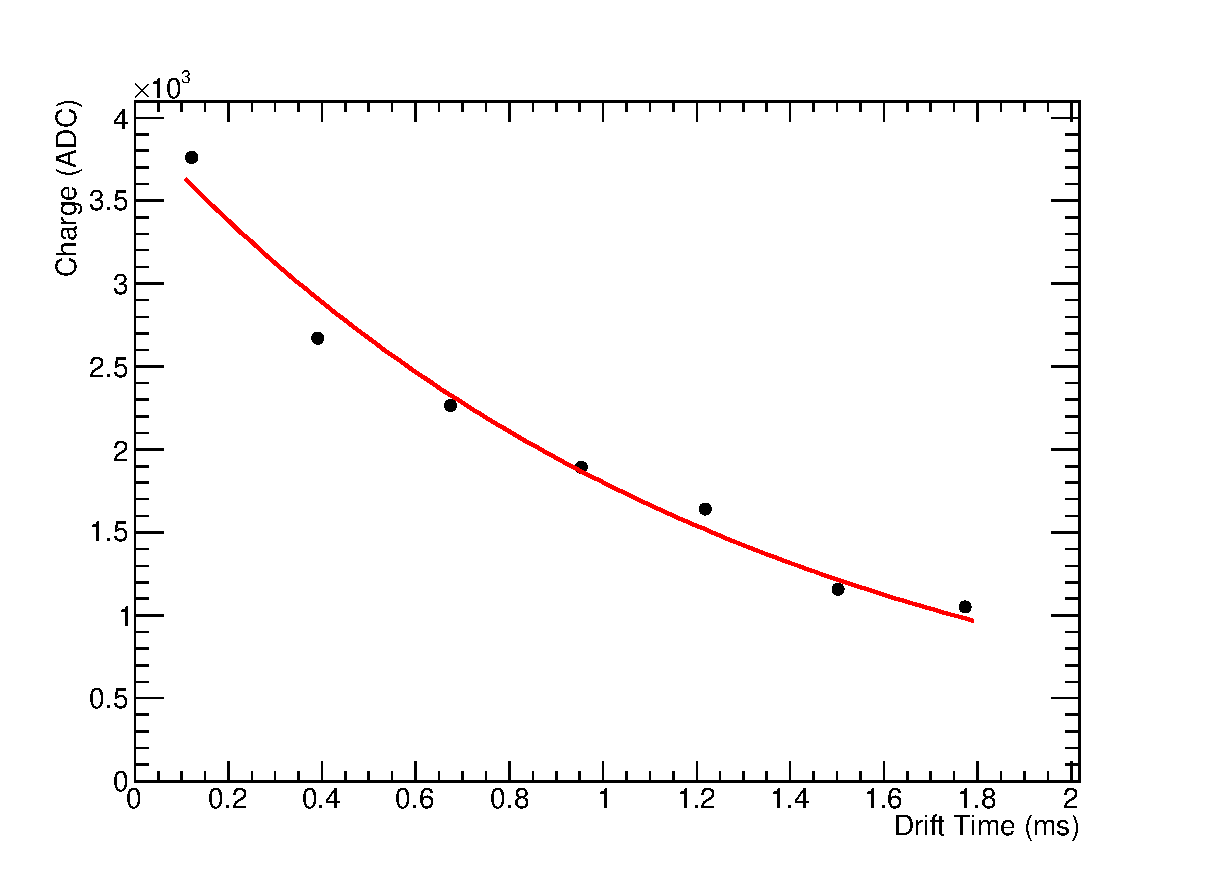
\includegraphics[width=12cm]{Purity.eps}
%%   \caption{}
%%   \label{fig:ElectronLifetimeData}
%% \end{figure}

%----------------------------------------------------------------------------------------------------------------------------------------------------------------------------
\section{APA Gap-Crossing Muons}\label{sec:APAGapCrossing}

One of the primary motivations for the design of the 35-ton TPC was to test its modular form, where a single drift region is read out by multiple anode assemblies.  Particles passing through the detector will leave deposits in multiple DVs and will pass uninstrumented regions of the detector, such as gaps in between neighbouring APAs; some example tracks are demonstrated in Figure~\ref{fig:35tonCounters}.  Many APA gap-crossing tracks are evident from the event display in Figure~\ref{fig:evd_crossing} and an example of such a track is depicted schematically in Figure~\ref{fig:APAGapCrosser}.  It is essential the implications of this design choice are understood before constructing the far detector modules, each of which will contain 150 APAs.

\begin{figure}
  \centering
  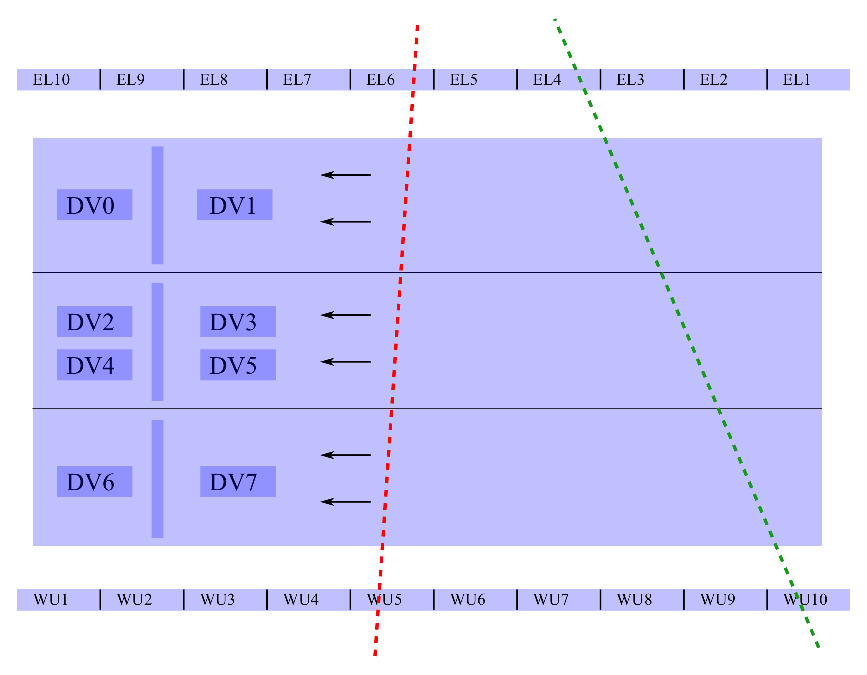
\includegraphics[width=10cm]{CounterGradient.eps}
  \caption[Demonstration of crossing muons tracks in the 35-ton TPC.]{Demonstration of crossing muon tracks in the 35-ton TPC.  The view is from the top of the cryostat looking down, with EW counters shown on either side of the TPC.  The APAs, defining the eight DVs, are represented by the darker rectangles towards the left of the detector.  The `counter gradient' is defined as the angle a track makes with respect to the face of the APAs.  Two example tracks are shown; the red track has a counter gradient of zero whilst the green track has a gradient of three.}
  \label{fig:35tonCounters}
\end{figure}

\begin{figure}
  \centering
  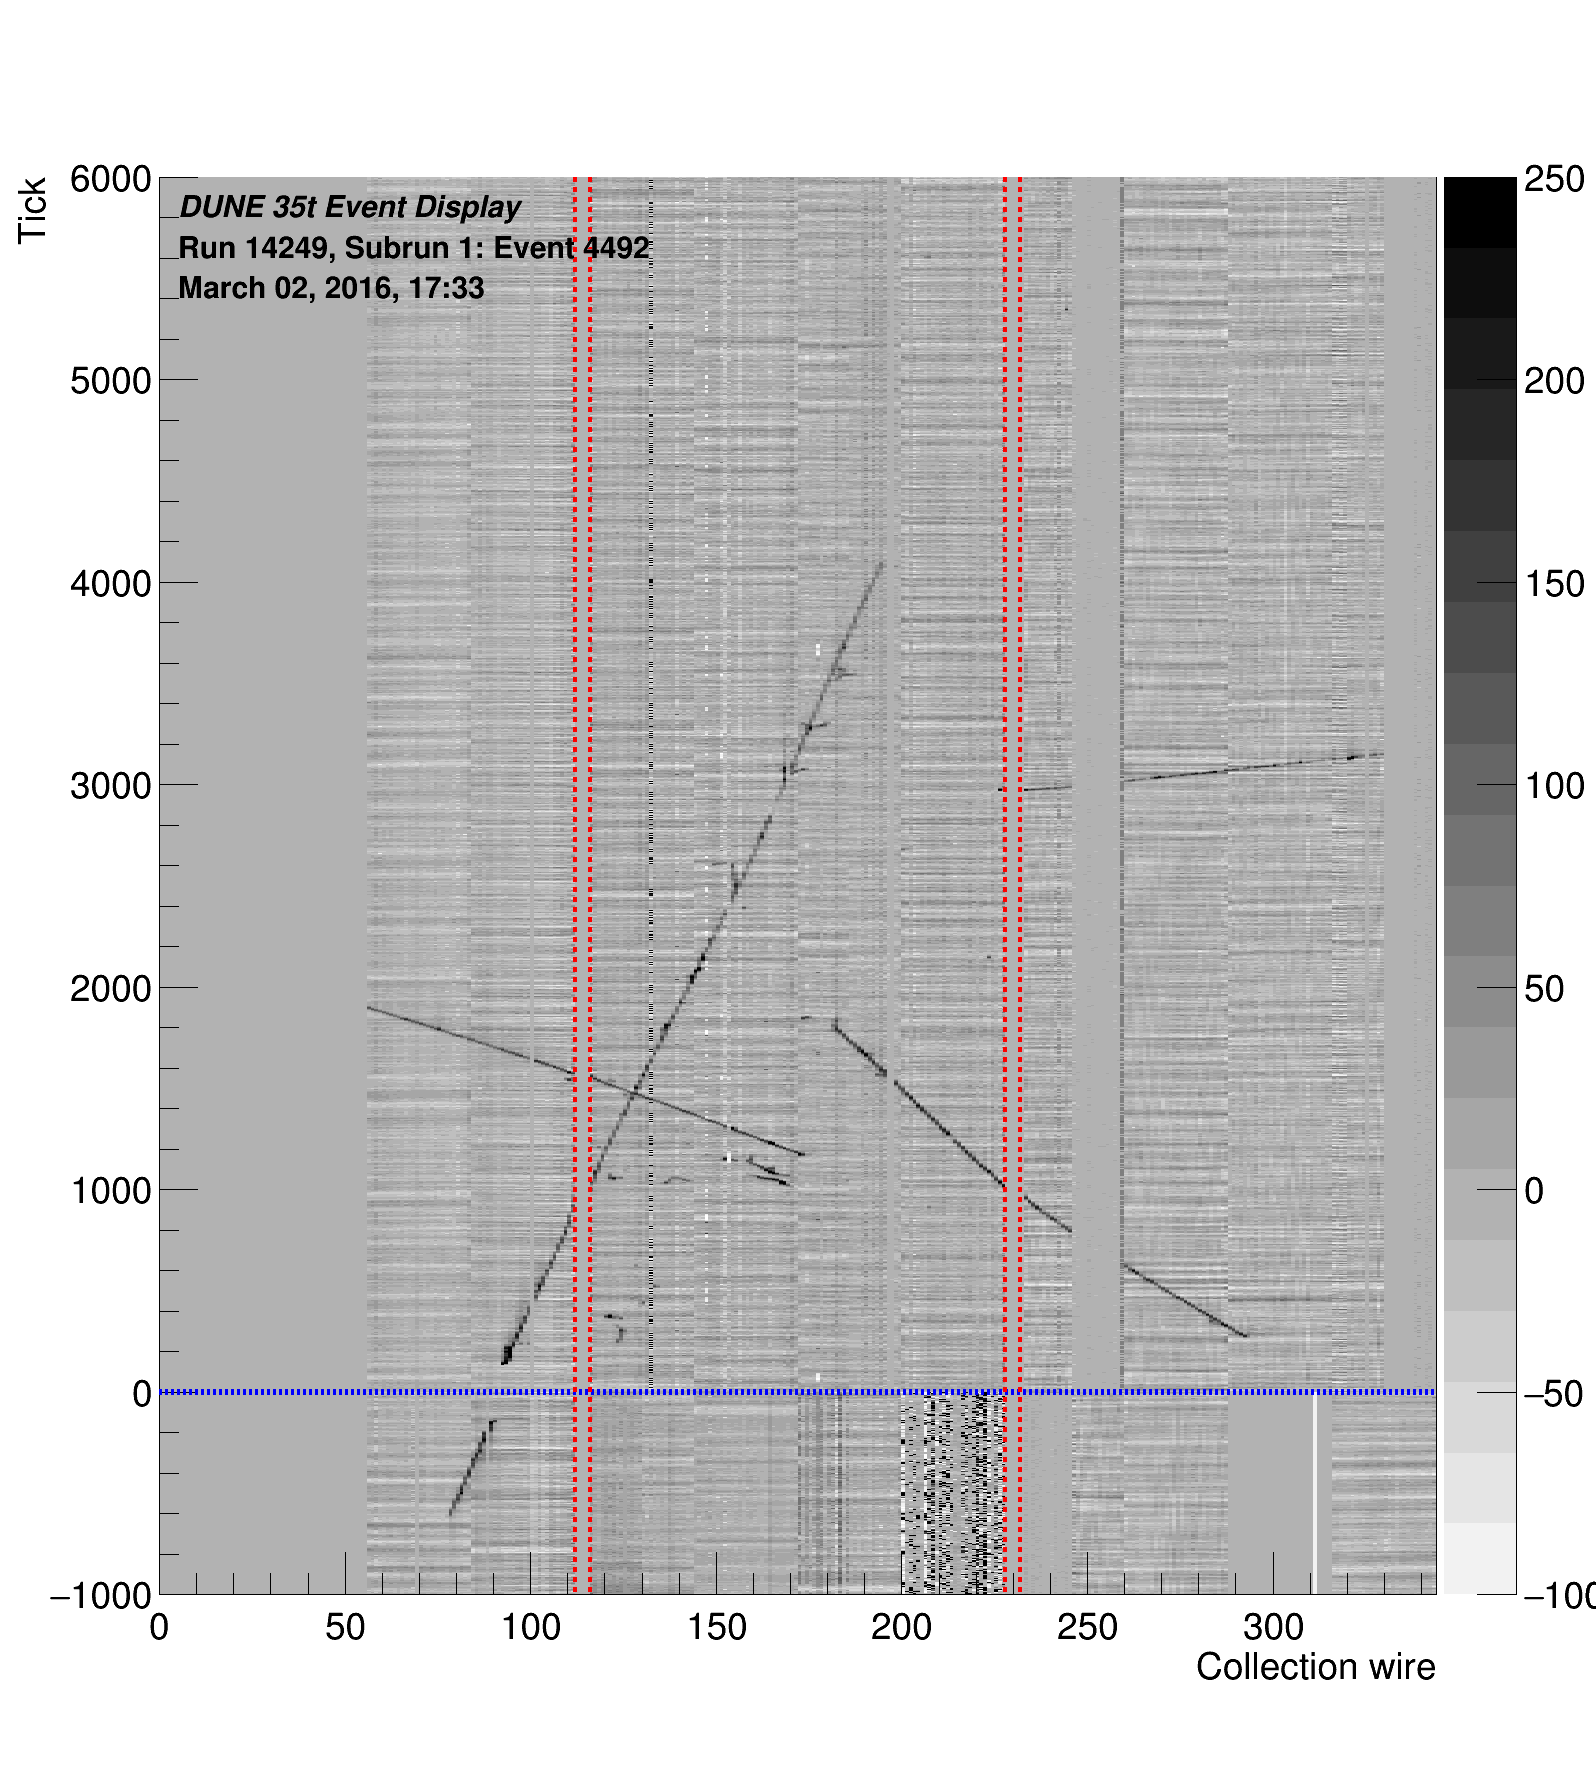
\includegraphics[width=12cm]{evd_run14249_subrun1_event4492.png}%evd_t0_2.pdf}
  \caption[Event display showing tracks passing across APA gaps and also through the APAs.]{Event display showing tracks passing across APA gaps and also through the APAs.  A study of the tracks which pass across gaps between the APAs (the red lines) is the subject of Section~\ref{sec:APAGapCrossing}.  There is a visible offset apparent as the track crosses through the APAs (the blue line); correcting for T0 would eliminate this and yield a single accurately connected track.  This is discussed further in Section~\ref{sec:APACrossing}.}
  \label{fig:evd_crossing}
\end{figure}

\begin{figure}
  \centering
  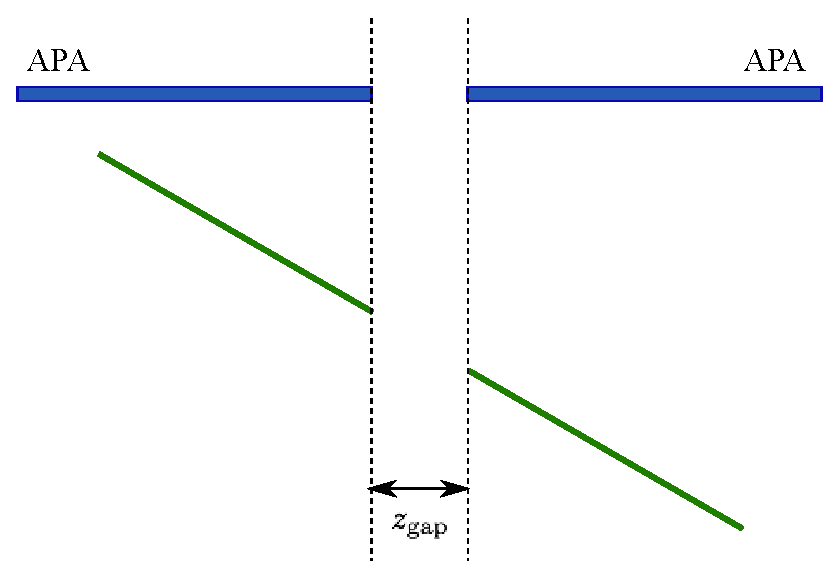
\includegraphics[width=8cm]{apa_gap.eps}
  \caption[Schematic showing an example APA gap-crossing track as viewed looking down from the top of the detector.]{Schematic showing an example APA gap-crossing track as viewed looking down from the top of the detector.  The vertical direction represents the drift direction ($x$); the horizontal direction represents the $z$-direction.  In general, these tracks make an angle with respect to the face of the APAs, as shown in the figure.  As the gap in between the APAs is uninstrumented, no charge is deposited in this region.}
  \label{fig:APAGapCrosser}
\end{figure}

The 35-ton dataset consisting of muons which pass across the face of APAs and therefore deposit charge in consecutive DVs is discussed in this present section.  An analysis of these tracks to calculate the size of the gaps is presented in Section~\ref{sec:APAGapOffsets} and a study of the charge deposited by such tracks is the subject of Section~\ref{sec:APAGapCharge}.

%----------------------------------------------------------------------------------------------------------------------------------------------------------------------------
\subsection{APA-Gap Offset Determination}\label{sec:APAGapOffsets}

It is possible to use these gap-crossing tracks to make measurements of the gaps between each of the APAs.  This involves aligning the track segments from neighbouring DVs, demonstrated in Figure~\ref{fig:APAGapZOffset}.  The value of the $z$-offset, $\Delta z$, is determined by considering a range of offset hypotheses, performing a linear fit and finding the offset which minimises the residual least squares
\begin{equation}
  L = \sum_i^{nhits} (o_i - e_i)^2,
\end{equation}
where $o_i-e_i$ is the distance from hit $i$ to the best fit line.

\begin{figure}
  \centering
  \begin{subfigure}[t]{0.48\linewidth}
    \centering
    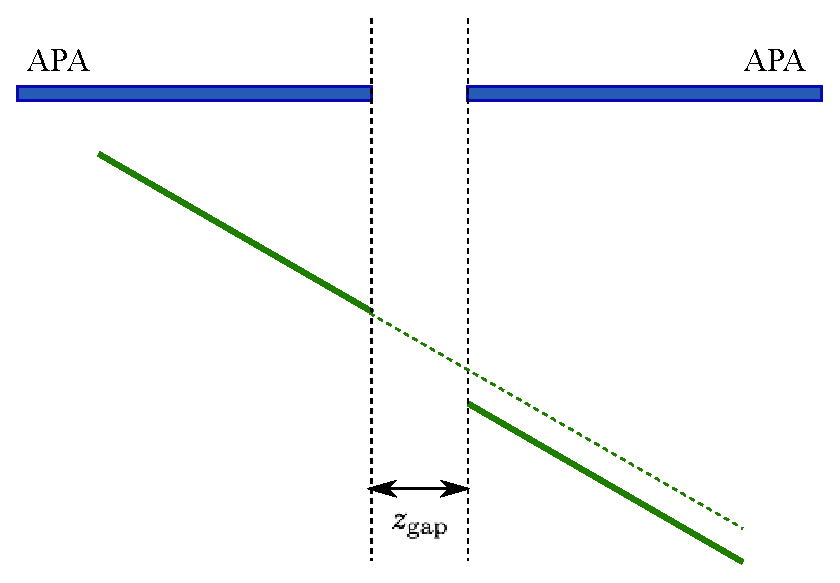
\includegraphics[width=0.92\textwidth]{apa_gap_zoffset.eps}
    \caption{Before correcting for $\Delta z$.}
    \label{fig:APAGapZOffsetUncorrected}
  \end{subfigure}
  \hfill
  \begin{subfigure}[t]{0.48\linewidth}
    \centering
    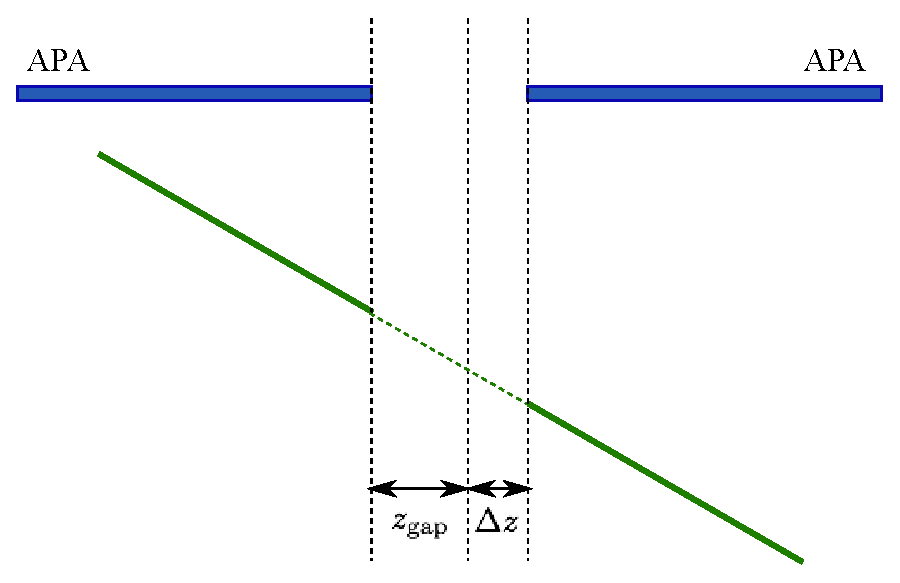
\includegraphics[width=0.98\textwidth]{apa_gap_zoffset_fix.eps}
    \caption{After correcting for $\Delta z$.}
    \label{fig:APAGapZOffsetCorrected}
  \end{subfigure}
  \caption[Schematic showing an example track crossing two drift regions offset by an unknown quantity $\Delta z$.]{Schematic showing an example track crossing two drift regions offset by an unknown quantity $\Delta z$.  The effect of this is evident from the track deposits (Figure~\ref{fig:APAGapZOffsetUncorrected}) and can be corrected by ensuring the segments are aligned between the DVs (Figure~\ref{fig:APAGapZOffsetCorrected}).}
  \label{fig:APAGapZOffset}
\end{figure}

There are eight gaps which can be measured from the data, demonstrated in Figure~\ref{fig:APAGapCrossingGaps}.  Due to very low statistics, it was found measurements of the gaps on the short drift volume side of the APAs were not possible using the 35-ton data.  Analysis of the gaps using tracks passing through the long drift volume, hereafter named DV1/DV3, DV1/DV5, DV3/DV7 and DV5/DV7, was therefore the focus of this study.

\begin{figure}
  \centering
  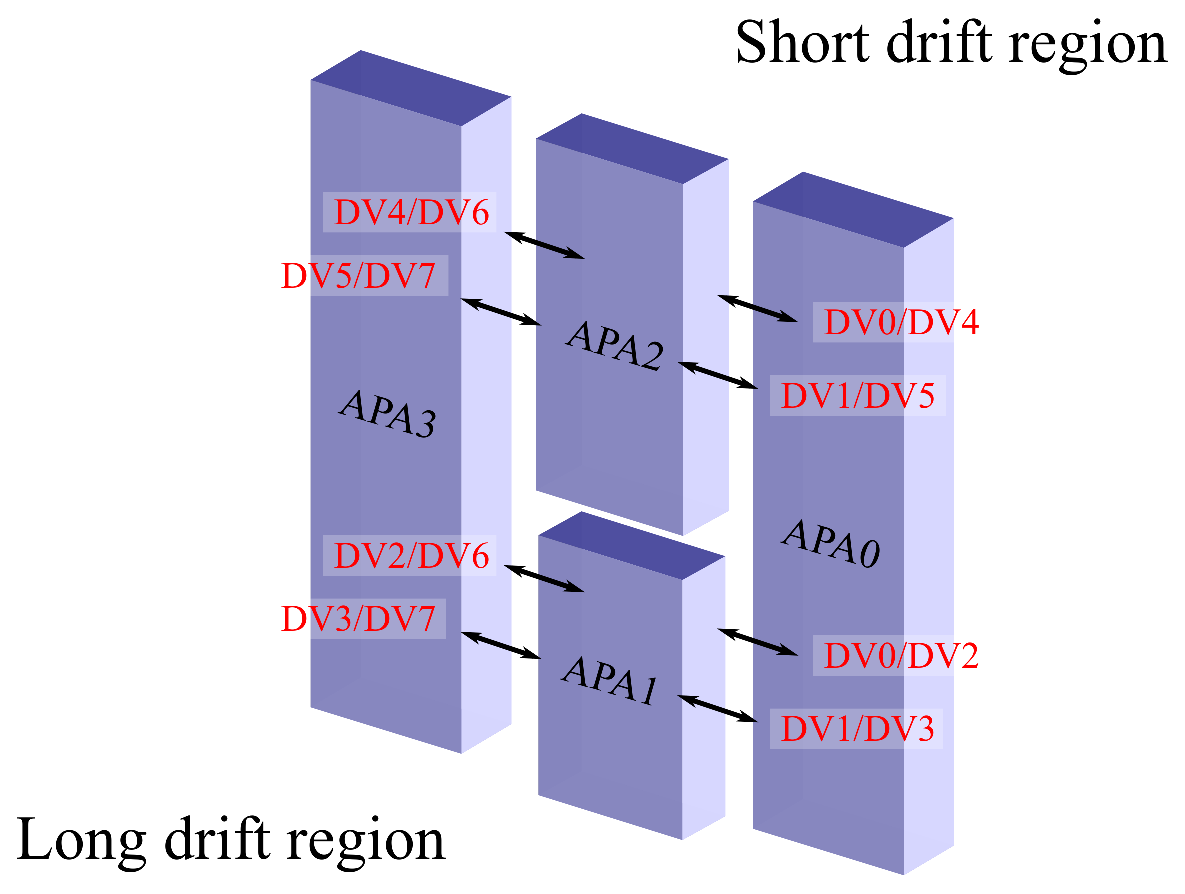
\includegraphics[width=12cm]{APAGapCrossingGaps.eps}
  \caption{Illustration of the eight gaps between the four APA frames.  There are four spaces between the APAs giving rise to eight gaps, measured in the long drift (odd-numbered) and short drift (even-numbered) regions.  In the figure, the even-numbered gaps represent the distance between the APAs on the back-facing side and the odd-numbered gaps the distance on the side facing.  Naively, one would expect the gaps to be identical but this will not necessarily be the case when assembled in the cryostat and, since they read out data from distinct drift regions, they may be considered separately.}
  \label{fig:APAGapCrossingGaps}
\end{figure}

A number of cuts were applied to ensure only high quality tracks were included for analysis:
\begin{itemize}
  \item{Only hits greater than 1~cm and less than 15~cm away from the gap were included in the track segments.  The purpose of this cut is to limit the effect of multiple scatterings and the poorly understood region closest to the gap, where charge deposited in the uninstrumented region may later be collected.}
  \item{Each track segment must contain at least ten hits to allow an accurate measure of the gradient.}
  \item{The angle between the track segments either side of the gap must be less than 2$^\circ$ to remove any poorly reconstructed tracks, or segments originating from different particle tracks.}
  \item{The angle the track makes with respect to the APA face must be large enough that the gap offset effect can be measured to an acceptable accuracy.  It is common in the 35-ton to refer to a `counter gradient', the offset between the two counters forming the through-going particle trigger in the drift direction, in units of counter length (demonstrated in Figure~\ref{fig:35tonCounters}).  The tracks must have a counter gradient of at least three.}
\end{itemize}

%----------------------------------------------------------------------------------------------------------------------------------------------------------------------------
\subsubsection{Measuring the APA Gaps}\label{sec:MeasuringAPAGaps}

The gap which possesses the largest number of crossers is DV5/DV7 and so the procedure will be demonstrated using data from this channel.  The $z$-offset determined using the method and cuts described above is shown in Figure~\ref{fig:DV5DV7XOffsetZOffset}.  An unexpected feature is evident from this distribution; there is not a single peak but two, seemingly related to the angle which the through-going particle makes with respect to the APAs.

\begin{figure}
  \centering
  \begin{subfigure}[t]{\linewidth}
    \centering
    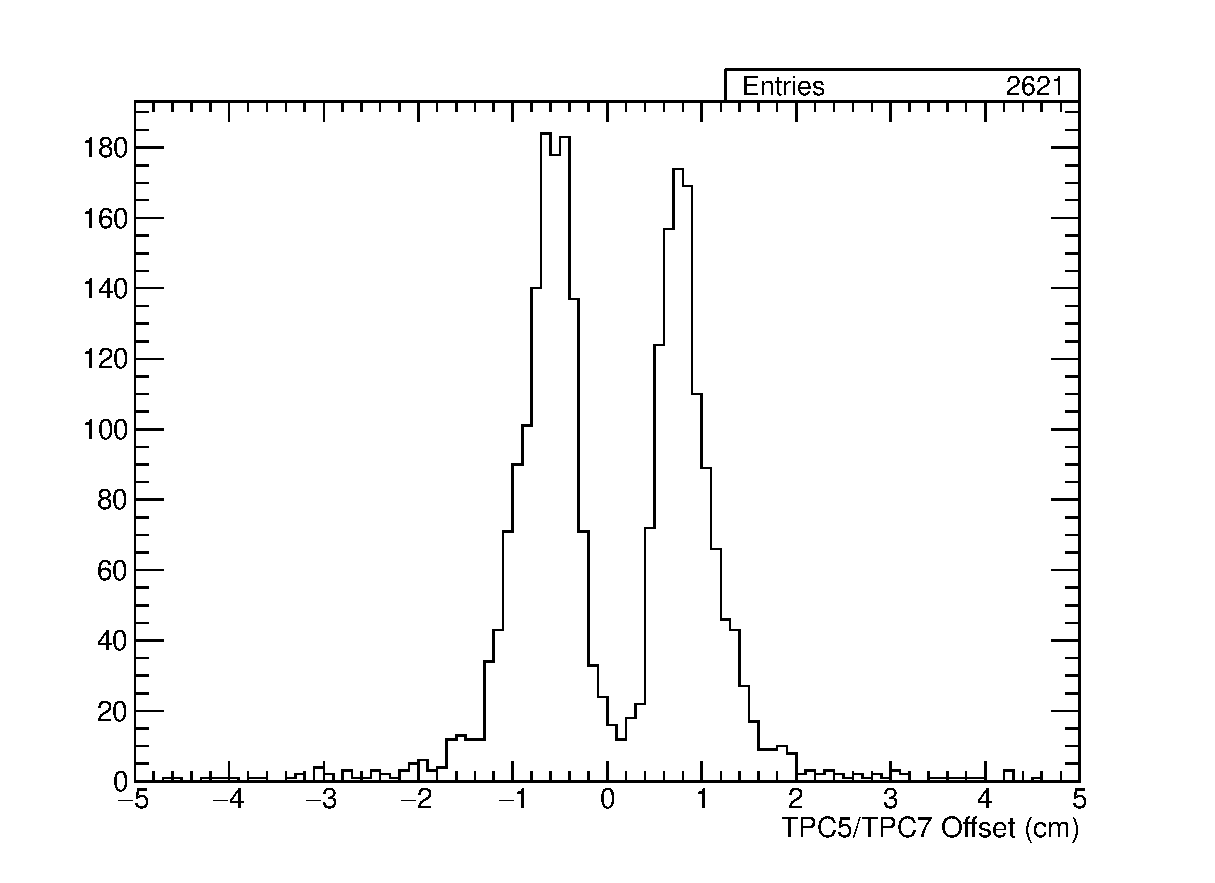
\includegraphics[width=12cm]{TPC5TPC7Gap.eps}
    \caption{Full distribution.}
    \label{fig:DV5DV7Gap}
  \end{subfigure}
  \hfill
  \begin{subfigure}[t]{\linewidth}
    \centering
    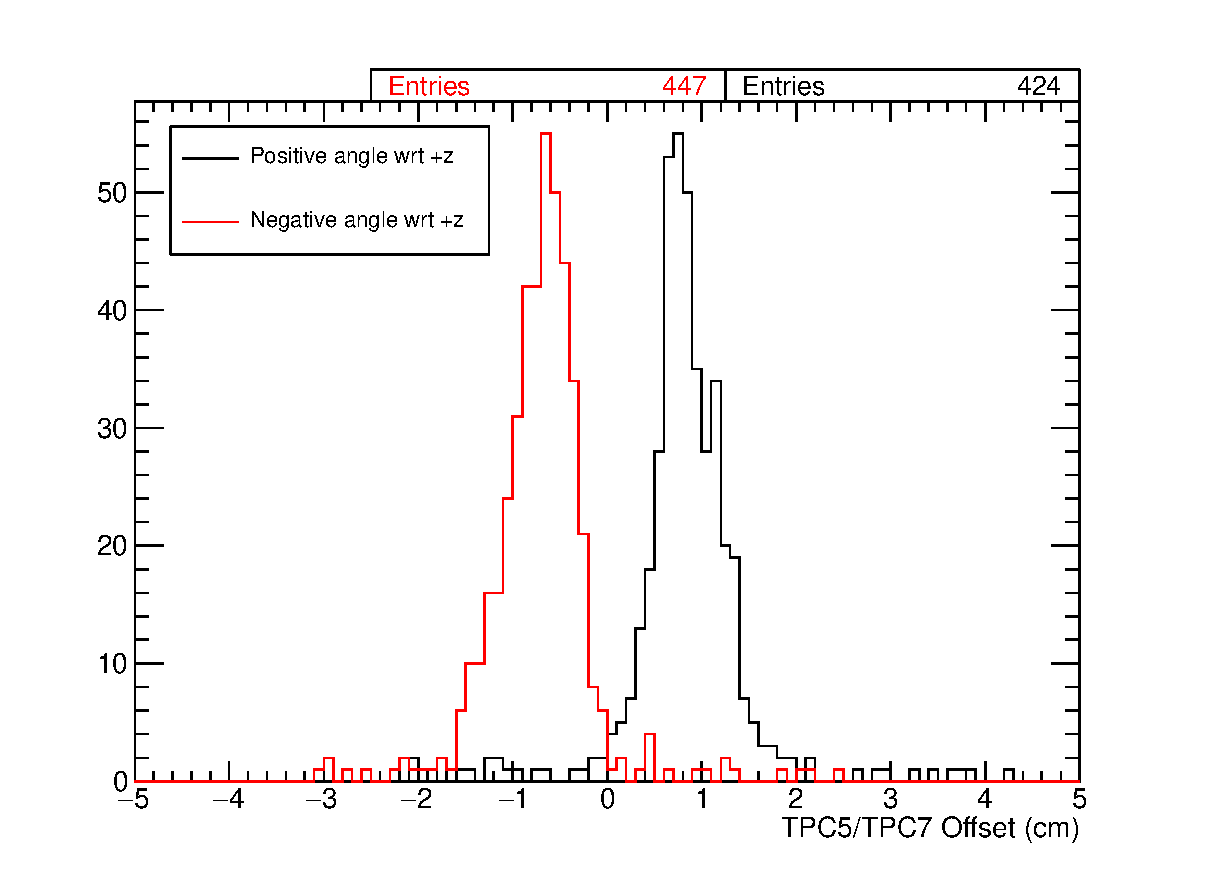
\includegraphics[width=12cm]{TPC5TPC7GapAngle.eps}
    \caption{Separated by the angle the track makes to the APAs.}
    \label{fig:DV5DV7GapAngle}
  \end{subfigure}
  \caption[The $z$-offset for the DV5/DV7 gap measured in the 35-ton data.]{The $z$-offset for the DV5/DV7 gap measured in the 35-ton data.  A very noticeable double-peak structure is evident in Figure~\ref{fig:DV5DV7Gap}; this bias appears to be related to the sign of the angle the particle track makes to the APA planes, demonstrated in Figure~\ref{fig:DV5DV7GapAngle}.}
  \label{fig:DV5DV7XOffsetZOffset}
\end{figure}

One explanation for this observed double-peak effect involves considering the possibility of additional offsets from the assumed positions of the APAs.  This is demonstrated in Figure~\ref{fig:APAGapXOffset}.  It appears an offset in the $x$-position of the APAs could result in the problems encountered in the data.  In order to test this, these offsets were artificially introduced into the simulation; the findings are presented in Figure~\ref{fig:APAGapMC}.  It appears the distribution of $\Delta z$ measured from the data is consistent with APAs with offsets from expectation in both $x$ and $z$.  Moreover, it may be possible to measure both offsets from the same data set.

\begin{figure}
  \centering
  \begin{subfigure}[t]{0.48\linewidth}
    \centering
    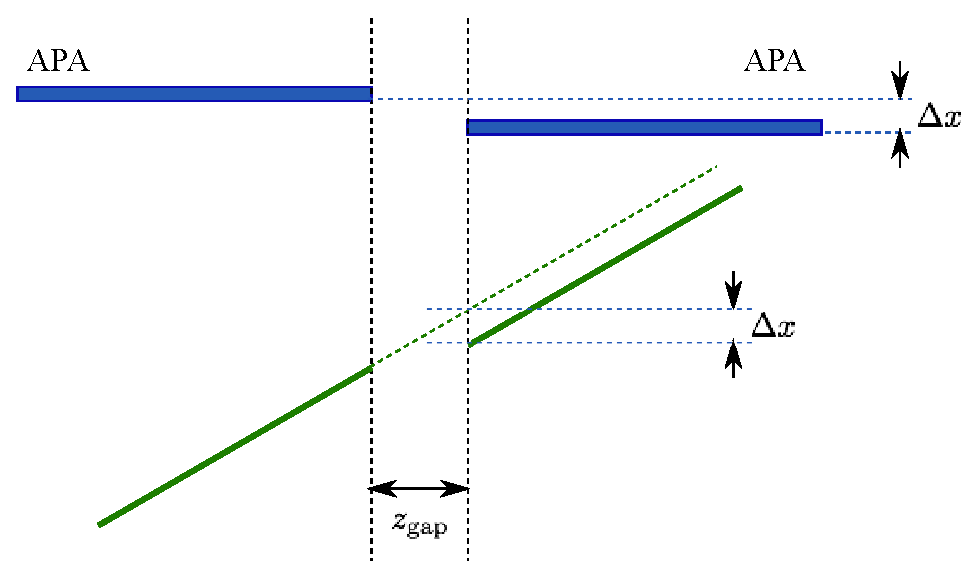
\includegraphics[width=0.98\textwidth]{apa_gap_xoffset_pos.eps}
    \caption{Positive track angle.}
    \label{fig:APAGapXOffsetPos}
  \end{subfigure}
  \hfill
  \begin{subfigure}[t]{0.48\linewidth}
    \centering
    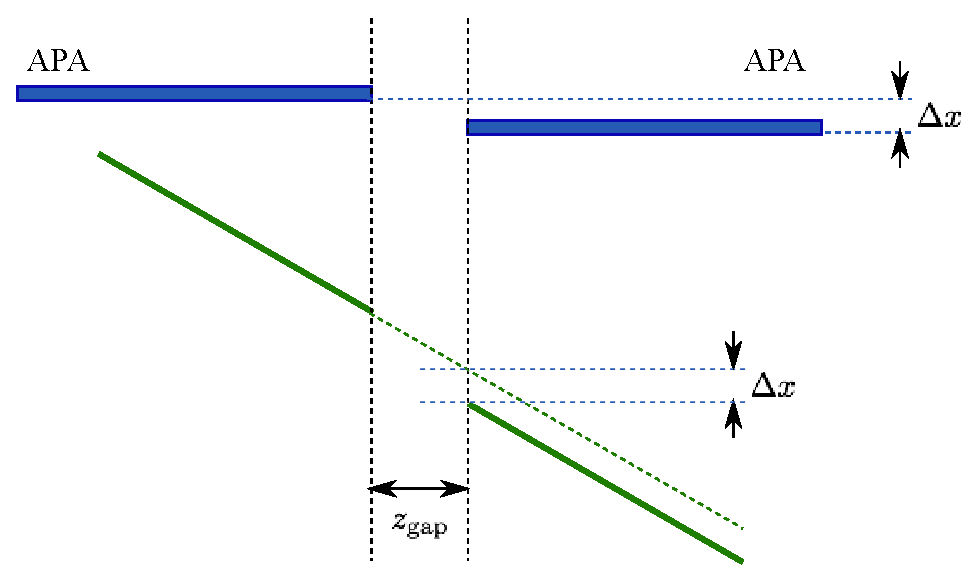
\includegraphics[width=0.98\textwidth]{apa_gap_xoffset_neg.eps}
    \caption{Negative track angle.}
    \label{fig:APAGapXOffsetNeg}
  \end{subfigure}
  \vfill
  \begin{subfigure}[t]{0.48\linewidth}
    \centering
    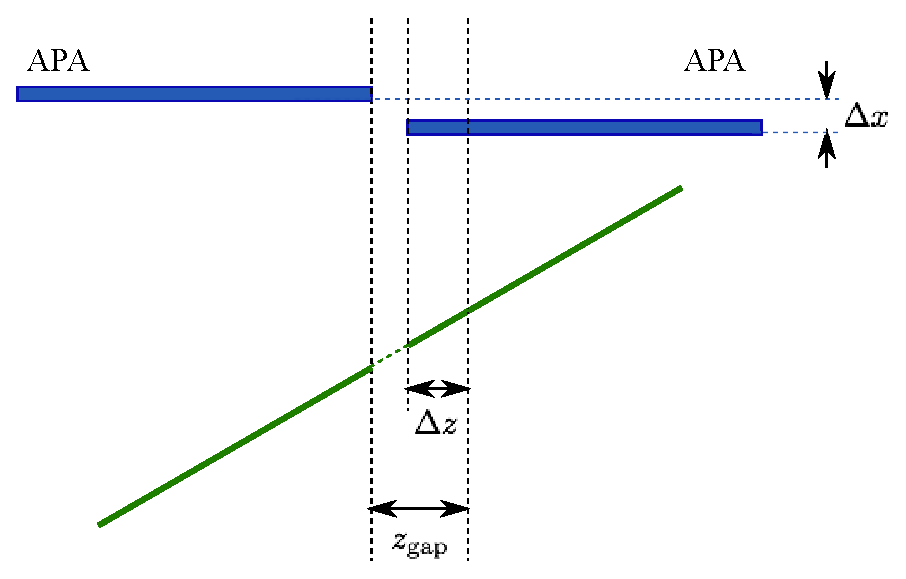
\includegraphics[width=0.98\textwidth]{apa_gap_xoffset_pos_fix.eps}
    \caption{Aligning the track segments gives a negative value of $\Delta z$ using the positive track.}
    \label{fig:APAGapXOffsetPosFix}
  \end{subfigure}
  \hfill
  \begin{subfigure}[t]{0.48\linewidth}
    \centering
    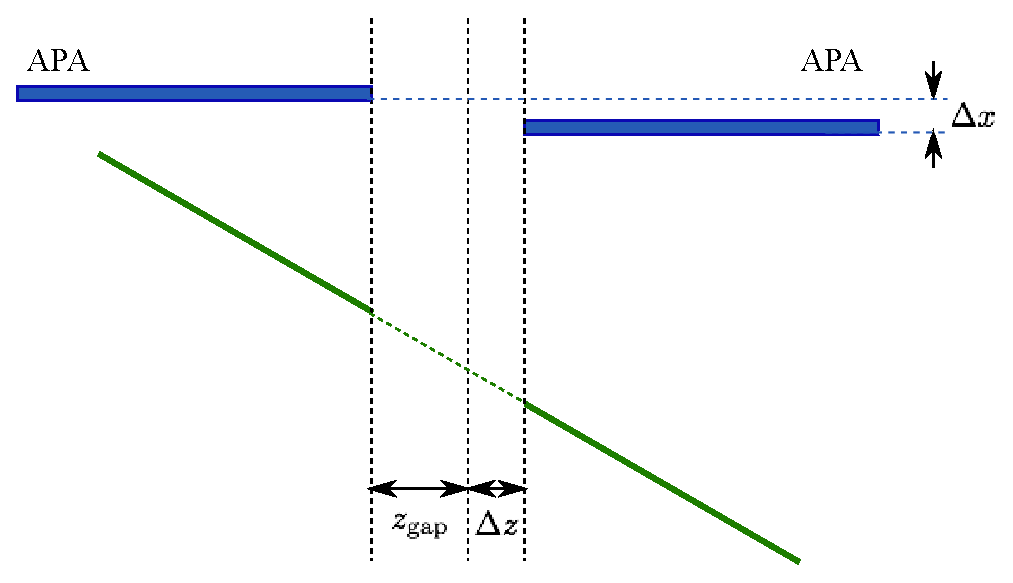
\includegraphics[width=0.98\textwidth]{apa_gap_xoffset_neg_fix.eps}
    \caption{Aligning the track segments gives a positive value of $\Delta z$ using the negative track.}
    \label{fig:APAGapXOffsetNegFix}
  \end{subfigure}
  \caption[Demonstration of how an $x$-offset in the positions of the APAs can explain the degeneracy evident in the $z$-offset measured using the 35-ton data.]{Demonstration of how an $x$-offset in the positions of the APAs can explain the degeneracy evident in the $z$-offset measured using the 35-ton data (Figure~\ref{fig:DV5DV7XOffsetZOffset}).  In the left-hand plots, Figures~\ref{fig:APAGapXOffsetPos} and~\ref{fig:APAGapXOffsetPosFix}, the through-going particle makes a positive angle to the face of the APAs and in the right-hand plots, Figures~\ref{fig:APAGapXOffsetNeg} and~\ref{fig:APAGapXOffsetNegFix}, the particle is travelling with a negative gradient.  In both cases, the offset of the APAs in the $x$-direction is the same.  It is clear from Figures~\ref{fig:APAGapXOffsetPosFix} and~\ref{fig:APAGapXOffsetNegFix} how the sign of the measured $\Delta z$ is dependent on the angle of the track.}
  \label{fig:APAGapXOffset}
\end{figure}

\begin{figure}
  \centering
  \begin{subfigure}[t]{\linewidth}
    \centering
    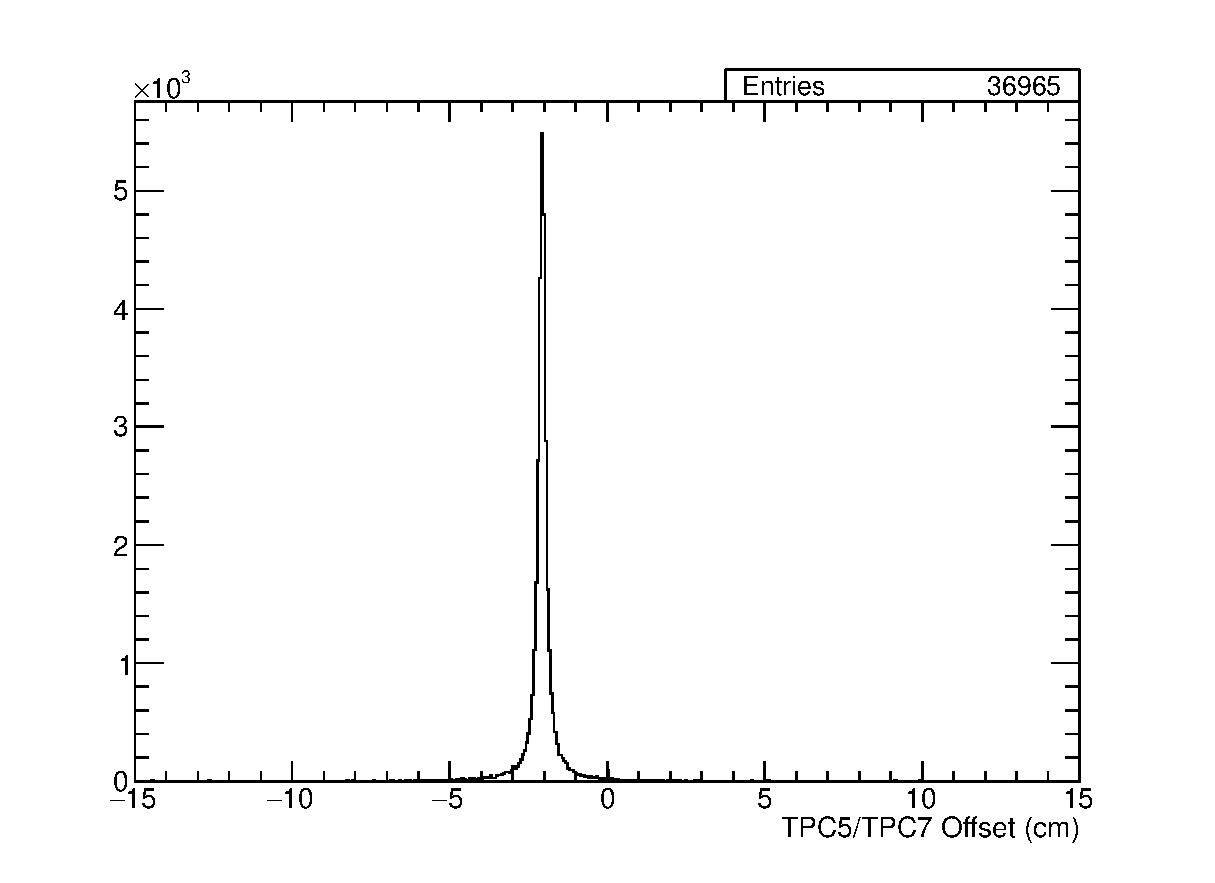
\includegraphics[width=8cm]{TPC5TPC7MCZOffset.eps}
    \caption{$z$-offset = 2~cm, $x$-offset = 0~cm.}
    \label{fig:APAGapMCZOffset}
  \end{subfigure}
  \hfill
  \begin{subfigure}[t]{\linewidth}
    \centering
    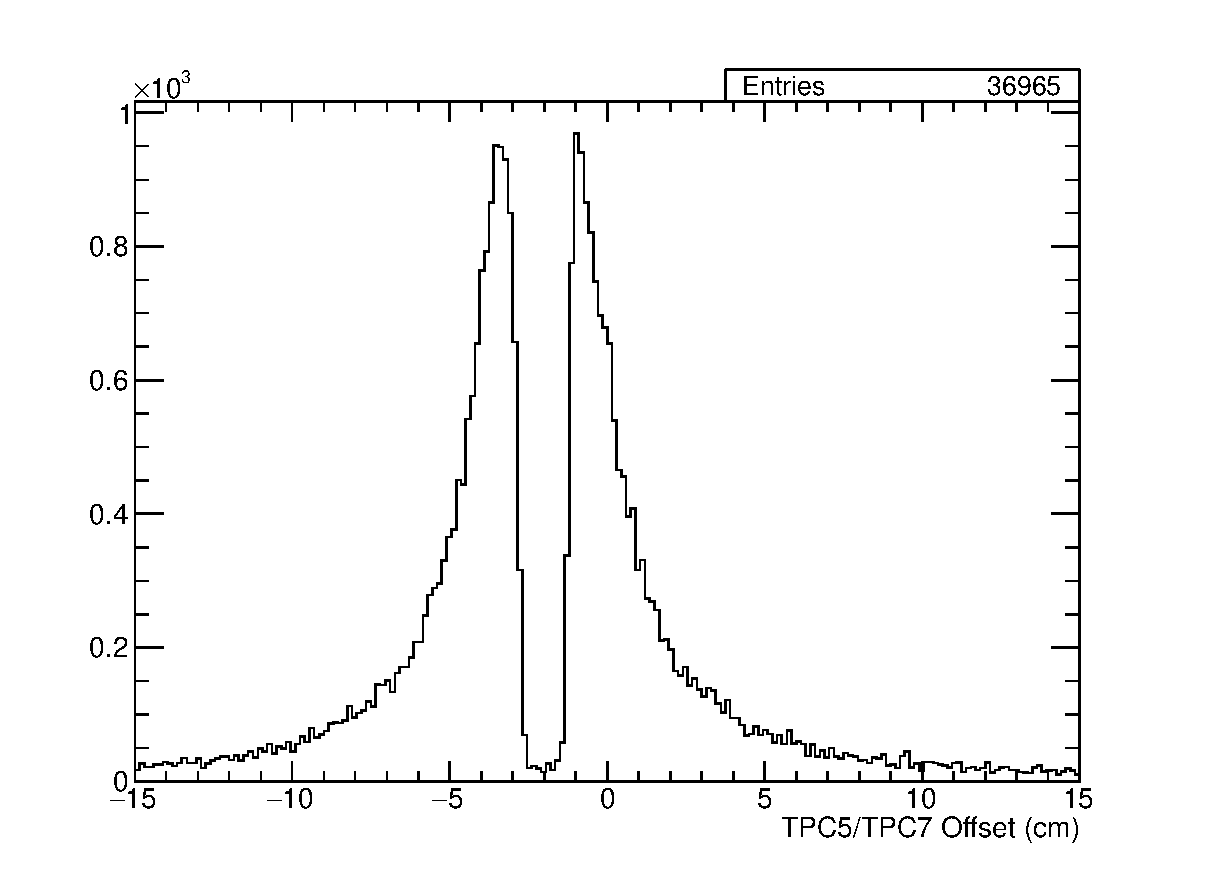
\includegraphics[width=8cm]{TPC5TPC7MCXOffsetZOffset.eps}
    \caption{$z$-offset = 2~cm, $x$-offset = 0.5~cm.}
    \label{fig:APAGapMCXOffsetZOffset}
  \end{subfigure}
  \hfill
  \begin{subfigure}[t]{\linewidth}
    \centering
    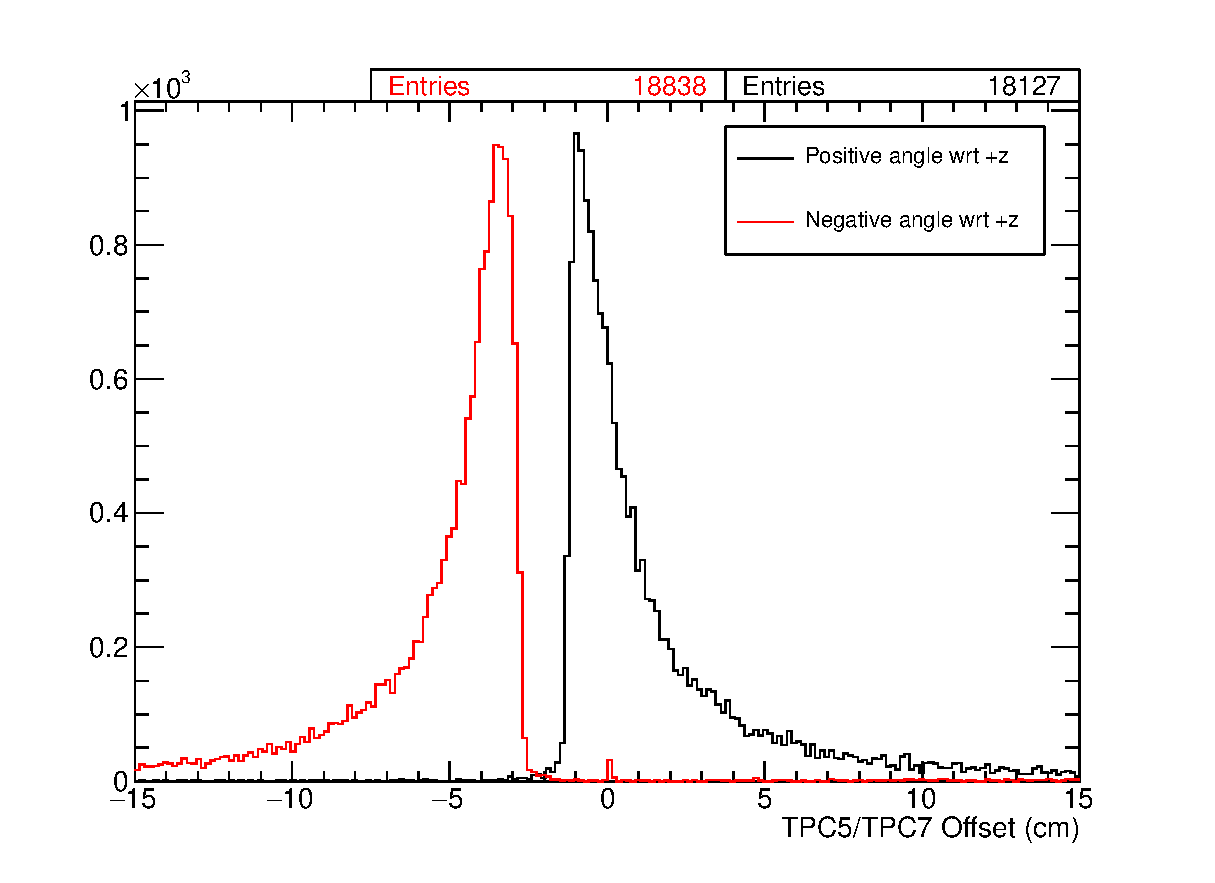
\includegraphics[width=8cm]{TPC5TPC7MCXOffsetZOffsetAngle.eps}
    \caption{$z$-offset = 2~cm, $x$-offset = 0.5~cm.}
    \label{fig:APAGapMCXOffsetZOffsetAngle}
  \end{subfigure}
  \caption[Studies of the effects of offsets in the positions of the APAs in simulation.]{Studies of the effects of offsets in the positions of the APAs in simulation.  Artificial $z$- and $x$- offsets are introduced and their impact observed in the measurements of $\Delta z$.  Figure~\ref{fig:APAGapMCZOffset} shows the effect of an offset in the $z$-direction; as expected, there is a single peak measuring the input value.  Figures~\ref{fig:APAGapMCXOffsetZOffset} and~\ref{fig:APAGapMCXOffsetZOffsetAngle} show the consequence of offsets in both the $x$- and $z$-directions.  This appears to show exactly what is seen in the 35-ton data (Figure~\ref{fig:DV5DV7XOffsetZOffset}).}
  \label{fig:APAGapMC}
\end{figure}

The offsets may be determined using a joint $\chi^2$ fit, in $\Delta z$-$\Delta x$ space, demonstrated in Figure~\ref{fig:DV5DV7CombinedOffsets}.  However, since hits are absolute and do not possess inherent positional uncertainties, it is particularly challenging estimating errors on the $\chi^2$ values, resulting in meaningless experimental uncertainties for the measured offsets.  Instead, since it is evident the offset values are uncorrelated, the process may be separated into two stages to ensure the uncertainties are correctly estimated.  This method will be the subject of the remainder of this section; the obtained values, in general, agree excellently with those extracted from simultaneous 2D fits.

\begin{figure}
  \centering
  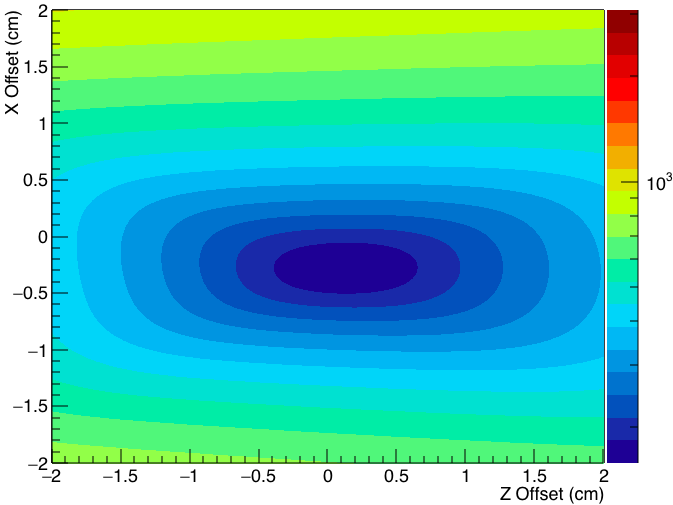
\includegraphics[width=10cm]{TPC5TPC7CombinedOffsets.png}
  \caption[The $\chi^2$ distribution for all APA-gap traversing tracks in $\Delta z$-$\Delta x$ space.]{The $\chi^2$ distribution for all APA-gap traversing tracks in $\Delta z$-$\Delta x$ space.}
  \label{fig:DV5DV7CombinedOffsets}
\end{figure}

It is clear from Figure~\ref{fig:APAGapMC} that the $z$-offset may be determined as the minimum between the angular-separated distributions.  This can be justified by geometrical considerations, explained in Figure~\ref{fig:APAGapXOffsetZOffset}.  In this case, this may be achieved by fitting a function of the form
\begin{equation}
  f(x) = a(x-b)^2+c
\end{equation}
and extracting parameter $b$ as the true value of $\Delta z$.  This is shown in Figure~\ref{fig:DV5DV7GapFit}.

\begin{figure}
  \centering
  \begin{subfigure}[t]{0.48\linewidth}
    \centering
    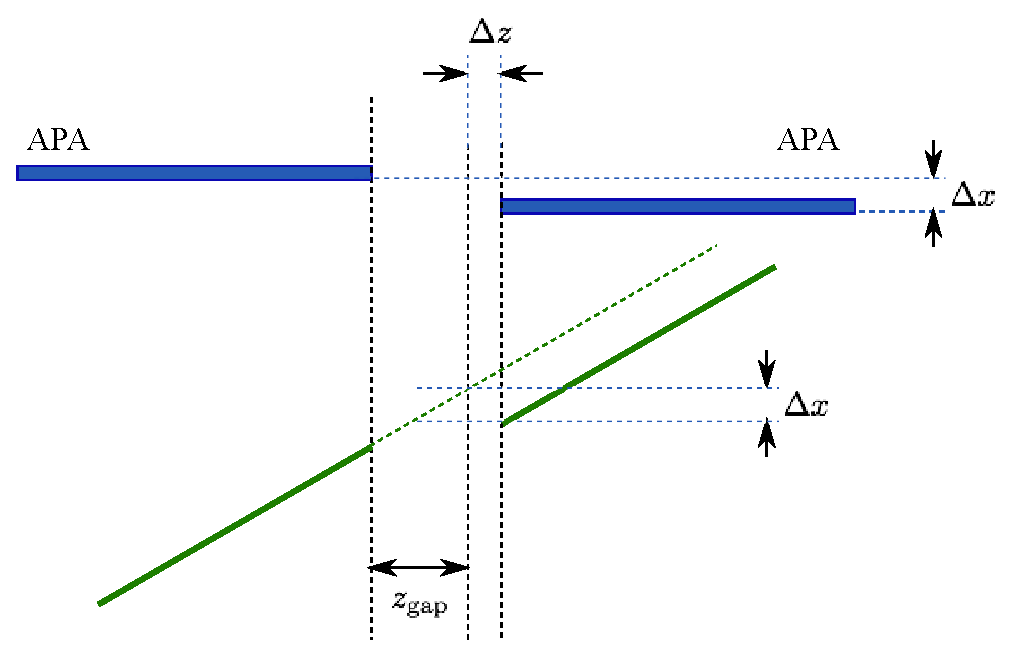
\includegraphics[width=0.98\textwidth]{apa_gap_xoffset_zoffset_pos.eps}
    \caption{Positive track angle.}
    \label{fig:APAGapXOffsetZOffsetPos}
  \end{subfigure}
  \hfill
  \begin{subfigure}[t]{0.48\linewidth}
    \centering
    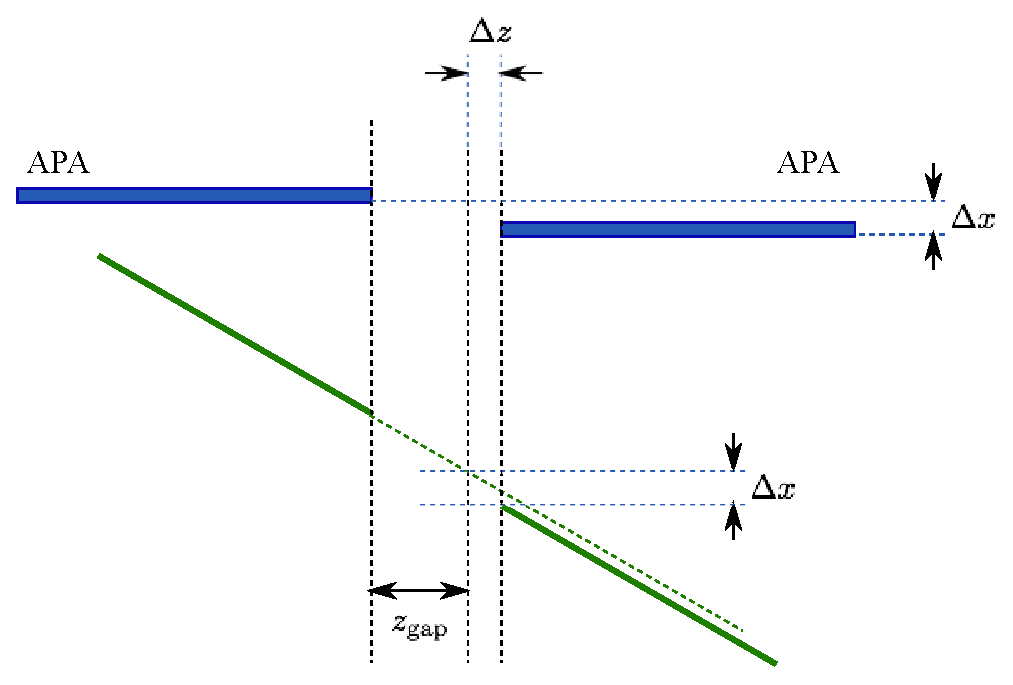
\includegraphics[width=0.98\textwidth]{apa_gap_xoffset_zoffset_neg.eps}
    \caption{Negative track angle.}
    \label{fig:APAGapXOffsetZOffsetNeg}
  \end{subfigure}
  \vfill
  \begin{subfigure}[t]{0.48\linewidth}
    \centering
    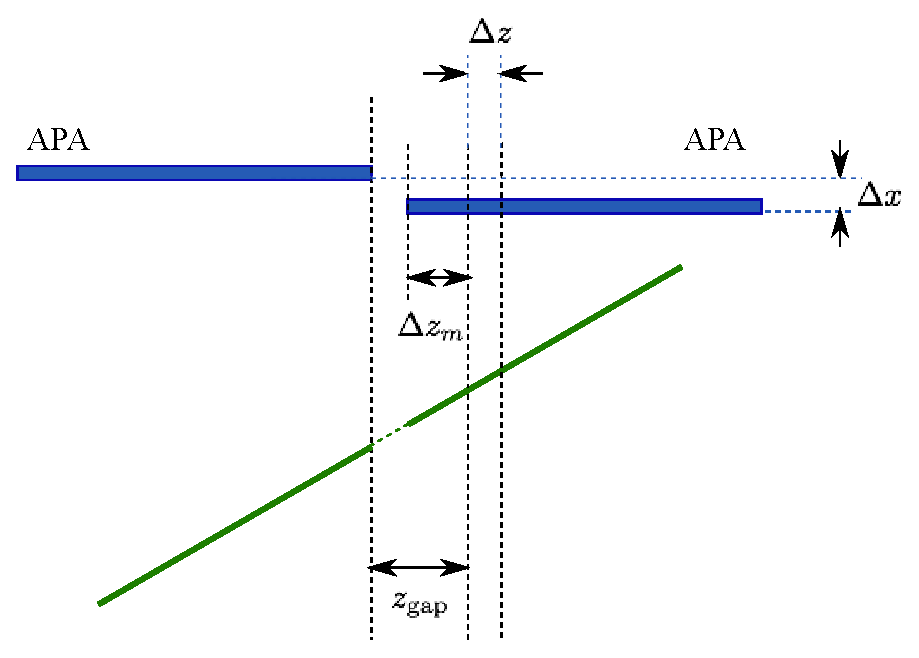
\includegraphics[width=0.98\textwidth]{apa_gap_xoffset_zoffset_pos_fix.eps}
    \caption{Aligning the track segments gives a measured $z$-offset, $\Delta z_m$, which is negative with an absolute value always greater than the true value.}
    \label{fig:APAGapXOffsetZOffsetPosFix}
  \end{subfigure}
  \hfill
  \begin{subfigure}[t]{0.48\linewidth}
    \centering
    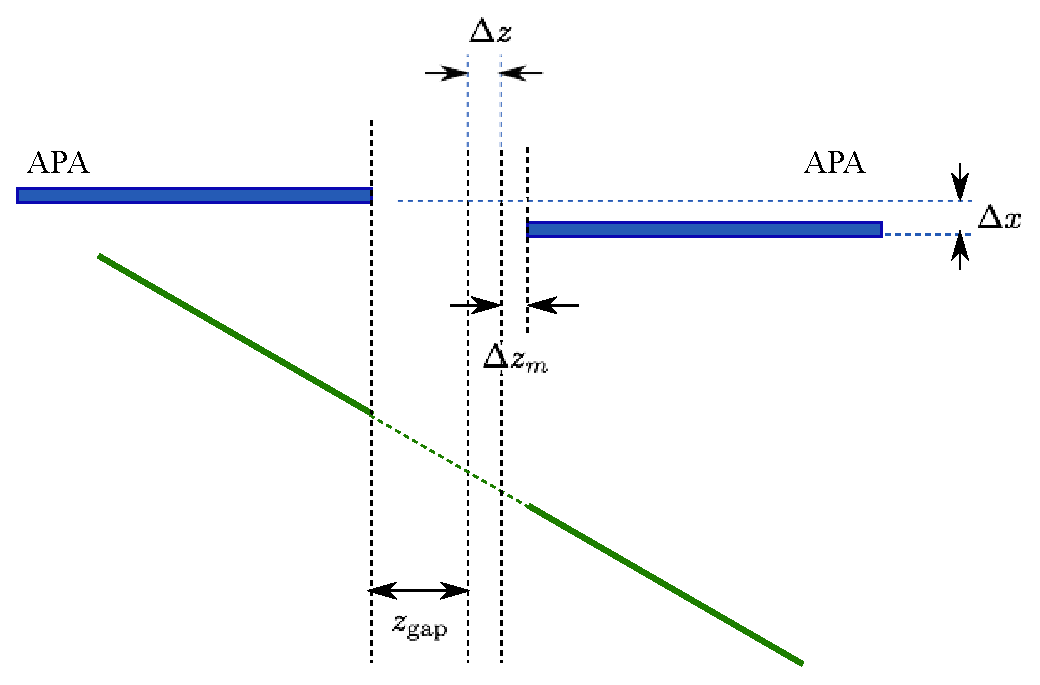
\includegraphics[width=0.98\textwidth]{apa_gap_xoffset_zoffset_neg_fix.eps}
    \caption{Aligning the track segments gives a measured $z$-offset, $\Delta z_m$, which is positive with an absolute value always less than the true value.}
    \label{fig:APAGapXOffsetZOffsetNegFix}
  \end{subfigure}
  \caption[Demonstration of the effects of offsets in both the $x$- and $z$-directions in the determination of $\Delta z$ between DV5 and DV7.]{Demonstration of the effects of offsets in both the $x$- and $z$-directions in the determination of $\Delta z$ between DV5 and DV7.  With an $x$-offset present, it is impossible for the true value of $\Delta z$ to be measured -- this is evident from Figure~\ref{fig:APAGapMC}.  It is clear from these geometrical considerations how the measured offset $\Delta z_m$ will populate distributions either side of the true value; the true value $\Delta z$ is given by the minimum between the two distributions.}
  \label{fig:APAGapXOffsetZOffset}
\end{figure}

\begin{figure}
  \centering
  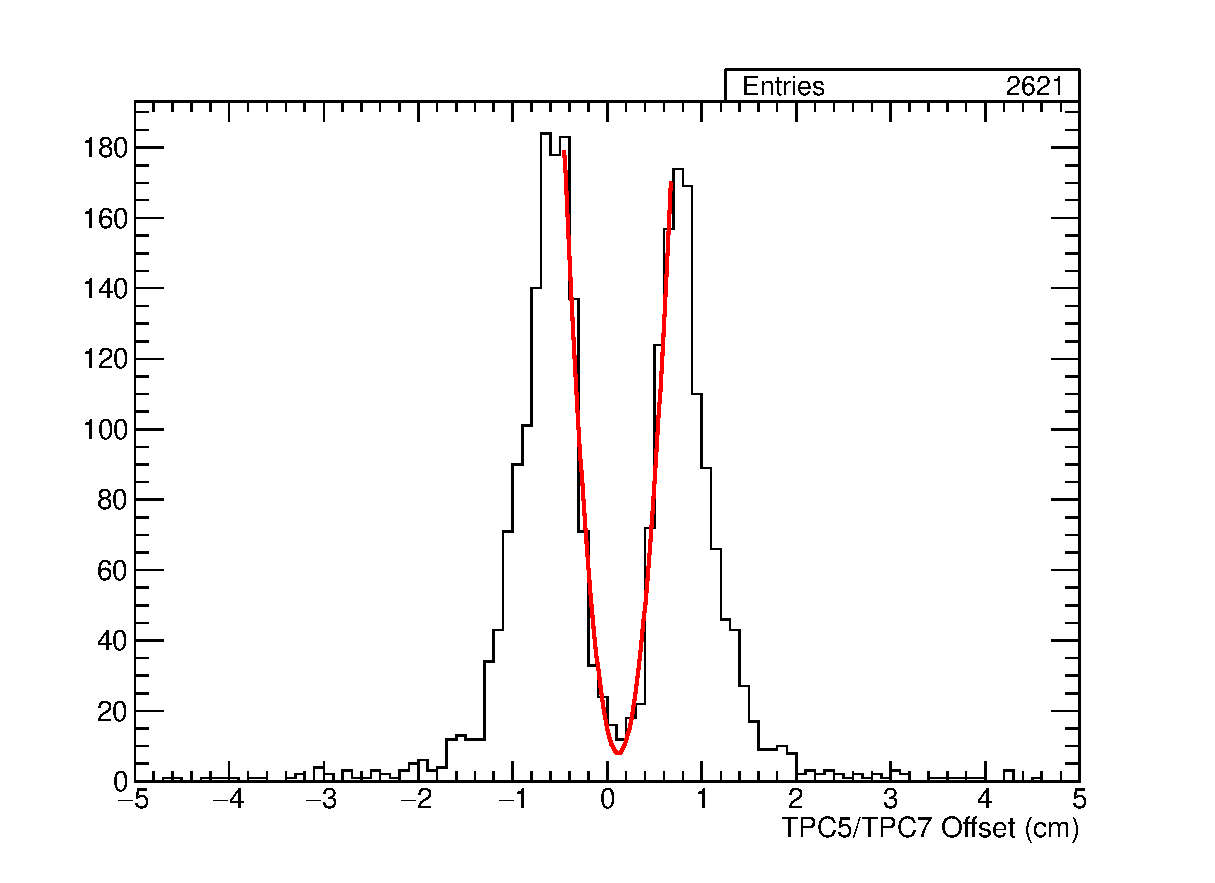
\includegraphics[width=12cm]{TPC5TPC7GapFit.eps}
  \caption[Extraction of the true value of $\Delta z$ from the full distribution of measured $z$-offsets.]{Extraction of the true value of $\Delta z$ from the full distribution of measured $z$-offsets.  A measured value of $0.117\pm0.007$~cm is found.}
  \label{fig:DV5DV7GapFit}
\end{figure}

Using this measured value of $\Delta z$, the offsets can be analysed again, this time measuring the $x$-offset by correcting for the $z$-offset.  The measured $x$-offset distribution is shown in Figure~\ref{fig:DV5DV7XOff}.  With this value of $\Delta x$, the $z$-offset can be evaluated once more to ensure the distribution contains a single peak, as initially expected.  This is confirmed in Figure~\ref{fig:DV5DV7ZOff}.

\begin{figure}
  \centering
  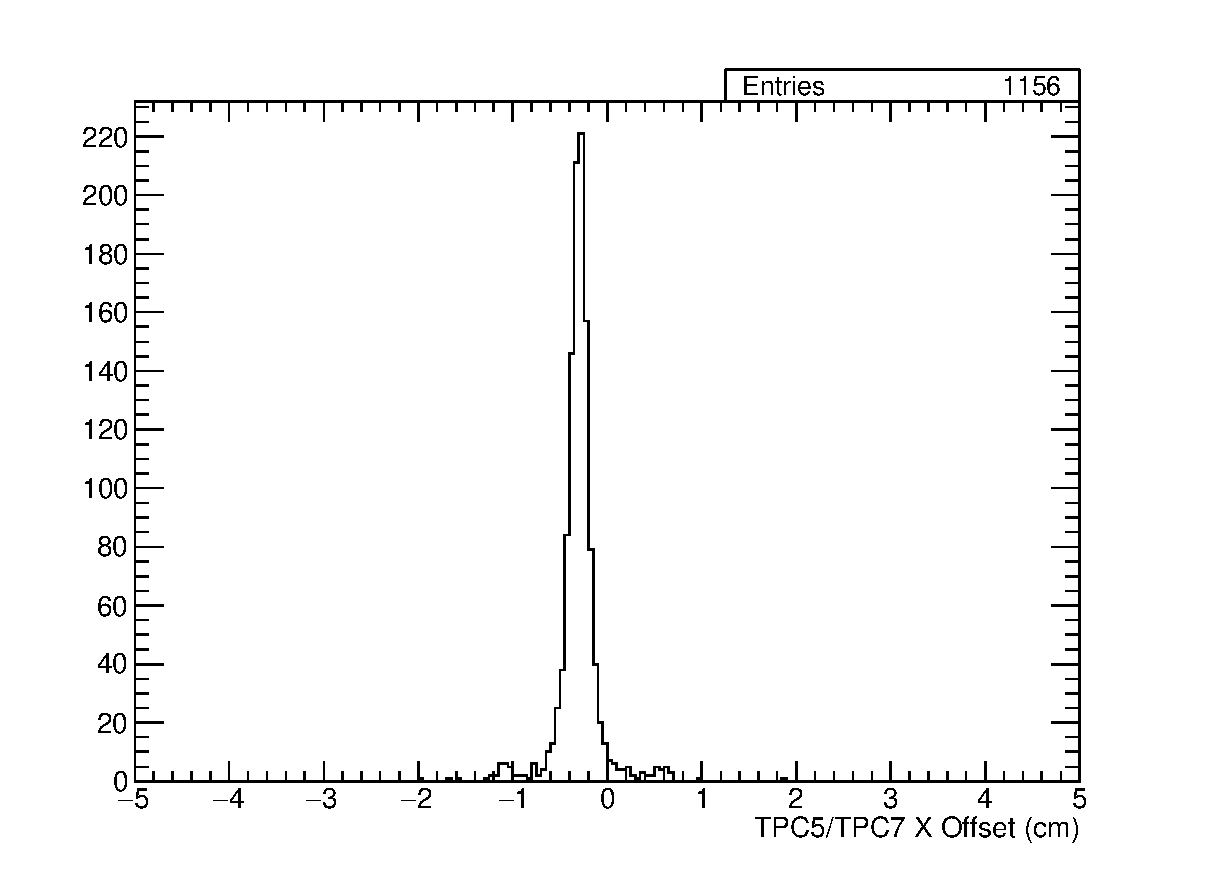
\includegraphics[width=12cm]{TPC5TPC7XOff.eps}
  \caption[Measurement of the $x$-offset between DV5 and DV7 after applying the $z$-gap correction.]{Measurement of the $x$-offset between DV5 and DV7 after applying the $z$-gap correction determined using the method described in the text and Figure~\ref{fig:DV5DV7GapFit}.  A measurement of $-0.286\pm0.002$~cm is determined.}
  \label{fig:DV5DV7XOff}
\end{figure}

\begin{figure}
  \centering
  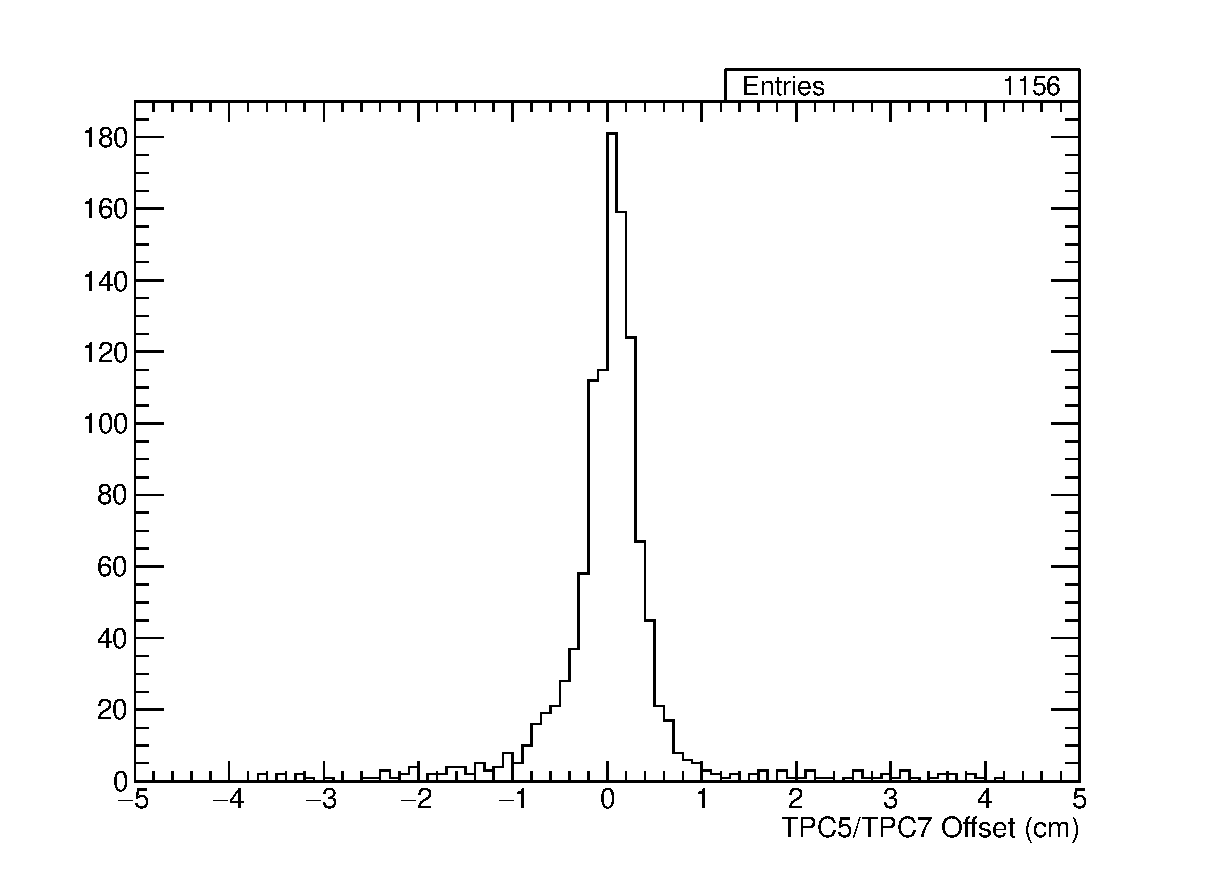
\includegraphics[width=12cm]{TPC5TPC7ZOff.eps}
  \caption[of the $z$-offset between DV5 and DV7 after applying the $x$-offset previously determined.]{Measurement of the $z$-offset between DV5 and DV7 after applying the $x$-offset determined from Figure~\ref{fig:DV5DV7XOff}.  As initially anticipated, there is a single peak distributed around the true value of the offset.  This validates the method used and confirms the initial presence of an $x$-offset between the neighbouring APAs.  The final measurement of $\Delta z$ is $0.103\pm0.004$~cm which agrees reasonably with the value measured previously ($0.117\pm0.007$~cm from Figure~\ref{fig:DV5DV7GapFit}).}
  \label{fig:DV5DV7ZOff}
\end{figure}

%----------------------------------------------------------------------------------------------------------------------------------------------------------------------------
\subsubsection{Measurements of the APA Offsets}\label{sec:APAOffsetMeasurements}

The offsets apparent from the data for all of the gaps accessible using TPC tracks in the long drift volume were determined as described in Section~\ref{sec:MeasuringAPAGaps}.  Appendix~\ref{appen:APAGap} contains all figures relevant for each gap measurement.  Table \ref{tab:APAOffsets} details all the measurements, and the new gaps are presented in Table \ref{tab:APAGaps} after taking all the offsets into account.  The determined errors are statistical only; the effects of systematic uncertainties were not considered and assumed to be negligible in comparison.

\begin{table}
  \centering
  \caption[Measurements of all the APA offsets determined from the 35-ton TPC data.]{Measurements of all the APA offsets determined from the 35-ton TPC data.  The method followed is described in Section~\ref{sec:MeasuringAPAGaps}.  The first row represents the initial measurements of the $z$-offset from the two-peak distribution, with the following two lines detailing the measured offsets that follow from these results.}
  \label{tab:APAOffsets}
%  \resizebox*{\columnwidth}{!}{
    \begin{tabular}{l  c  c  c  c }
      \toprule
      & DV1/DV3 & DV1/DV5 & DV3/DV7 & DV5/DV7 \\ %\hline\hline
      \midrule
      Initial $z$-offset (cm) & $-0.64 \pm 0.04$   & $0.15 \pm 0.01$    & $0.58 \pm 0.06$    & $0.117 \pm 0.007$  \\ %\hline
      $x$-offset (cm)         & $-0.377 \pm 0.006$ & $-0.252 \pm 0.002$ & $-0.16 \pm 0.01$   & $-0.286 \pm 0.002$ \\ %\hline
      $z$-offset (cm)         & $-0.63 \pm 0.02$   & $0.131 \pm 0.007$  & $0.55 \pm 0.03$    & $0.103 \pm 0.004$  \\
      \bottomrule
    \end{tabular}
 % }
  \vspace{3cm}
  \caption[The corrected gaps between the APAs, in $x$ and $z$, based on the offsets measured in the data.]{The corrected gaps between the APAs, in $x$ and $z$, based on the offsets measured in the data (Table \ref{tab:APAOffsets}).}
  \label{tab:APAGaps}
 % \resizebox*{\columnwidth}{!}{
    \begin{tabular}{l  c  c  c  c }
      \toprule
      & Assumed (cm) & Offset (cm) & Corrected (cm) \\ %\hline\hline
      \midrule
      DV1/DV3 $x$-gap & 0 & $-0.377 \pm 0.006$ & $-0.377 \pm 0.006$ \\
      DV1/DV5 $x$-gap & 0 & $-0.252 \pm 0.002$ & $-0.252 \pm 0.002$ \\
      DV3/DV7 $x$-gap & 0 & $-0.16  \pm 0.01$  & $-0.16  \pm 0.01$  \\
      DV5/DV7 $x$-gap & 0 & $-0.286 \pm 0.002$ & $-0.286 \pm 0.002$ \\
      \midrule
      DV1/(3)/DV7 $x$-gap & 0 & $-0.538 \pm 0.003$ & $-0.538 \pm 0.003$ \\
      DV1/(5)/DV7 $x$-gap & 0 & $-0.537 \pm 0.010$ & $-0.537 \pm 0.010$ \\
      \midrule
      DV1/DV3 $z$-gap & 2.08 & $-0.18 \pm 0.02$  & $1.90  \pm 0.02$  \\
      DV1/DV5 $z$-gap & 2.08 & $0.131 \pm 0.007$ & $2.211 \pm 0.007$ \\
      DV3/DV7 $z$-gap & 2.08 & $0.10  \pm 0.03$  & $2.18  \pm 0.03$  \\
      DV5/DV7 $z$-gap & 2.08 & $0.103 \pm 0.004$ & $2.183 \pm 0.004$ \\
      \midrule
      DV1/(3)/DV7 $z$-gap & 4.16 & $-0.08 \pm 0.04$ & $4.08 \pm 0.04$ \\
      DV1/(5)/DV7 $z$-gap & 4.16 & $0.23  \pm 0.01$ & $4.39 \pm 0.01$ \\
      \bottomrule
    \end{tabular}
  %}
\end{table}

Since there are two longer APAs either side of two short APAs, by combining the gap offset information from the gaps either side of the centre frames it is possible to make two implicit measurements of the offsets between the outer ones.  This is shown in Table~\ref{tab:APAGaps} for both the $x$- and $z$-offsets, with the number in brackets representing the DV across which the total gap offset was determined.  There appears to be some consistency in the measurements of the $x$-offsets between DV1 and DV7, found by considering the successive offsets between DV1/DV3 and DV3/DV7, and DV1/DV5 and DV5/DV7.  An exceptional agreement is seen between the two values, within 0.1~mm.  There also seems to be slight evidence of a rotation between DV1 and DV7 when considering the associated $z$-offsets; the offset at the top of the APA (when measured via DV5) is greater than at the bottom (when measured via DV3).  %cHowever, this can certainly be explained in the context of the limitations of the method and statistical fluctuations and would require more data and a more robust approach to justify these claims.  Such analysis is not possible with the 35-ton data.

The method demonstrated here will have direct implications for similar studies using the full DUNE far detector.  All the gaps between the APAs, both in the drift and $z$ directions, will need to be understood for accurate reconstruction and are essential in order for DUNE to make precise physics measurements.  For example, accurate calorimetric reconstruction is imperative in order to perform particle identification and shower energy determination (discussed in Section~\ref{sec:Calorimetry}) and is directly related to the drift time of the ionisation electrons; any offsets in APA positions will lead to systematic uncertainties in this information.

%----------------------------------------------------------------------------------------------------------------------------------------------------------------------------
\subsection{Charge Deposited by APA Gap-Crossing Muons}\label{sec:APAGapCharge}

The charge deposited by gap-crossing particles cannot be collected in the dead regions between the APA frames.  It is interesting to consider where the charge is read out in order to further understand the implications of a modular TPC design.

Figure~\ref{fig:HitGapDistance} demonstrates the properties of hits as a function of distance from the nearest DV edge.  It appears more hits are found as charge is collected near a gap but the charge of these hits do not differ significantly.  This may be interpreted as hits arriving at a slightly later time near the APA gaps after drifting towards the nearest wire to the gap from a more centre-gap position.  One may expect to observe this in the data as a smearing in the tick direction where charge is deposited over more time, leading to a small gradient change.  Although not as noticeable as anticipated, this effect is observable in the event display shown in Figure~\ref{fig:evd_gap}.

\begin{figure}
  \centering
  \begin{subfigure}[t]{0.48\linewidth}
    \centering
    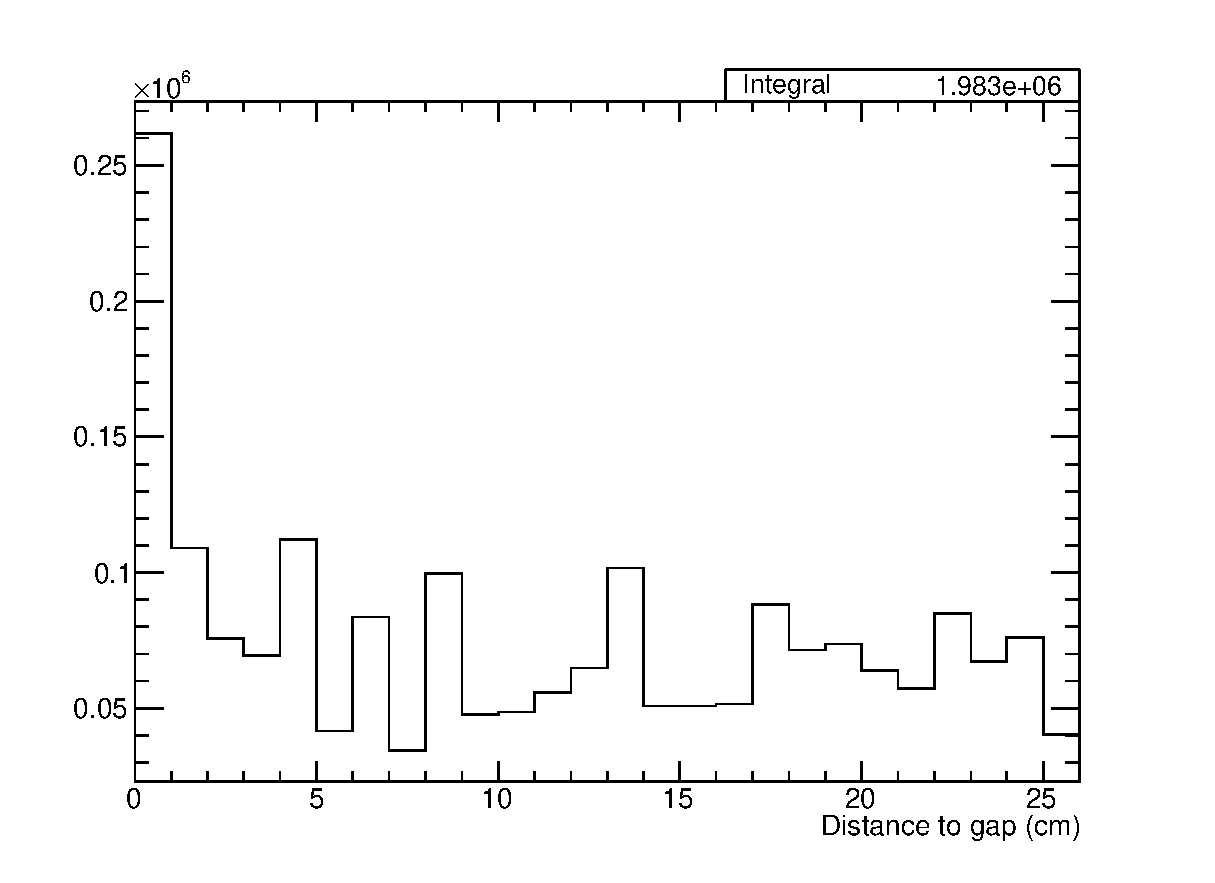
\includegraphics[width=0.98\textwidth]{HitGapDistance.eps}
    \caption{Number of reconstructed hits.}
    \label{fig:HitGapDistanceNum}
  \end{subfigure}
  %\vspace{1cm}
  \hfill
  \begin{subfigure}[t]{0.48\linewidth}
    \centering
    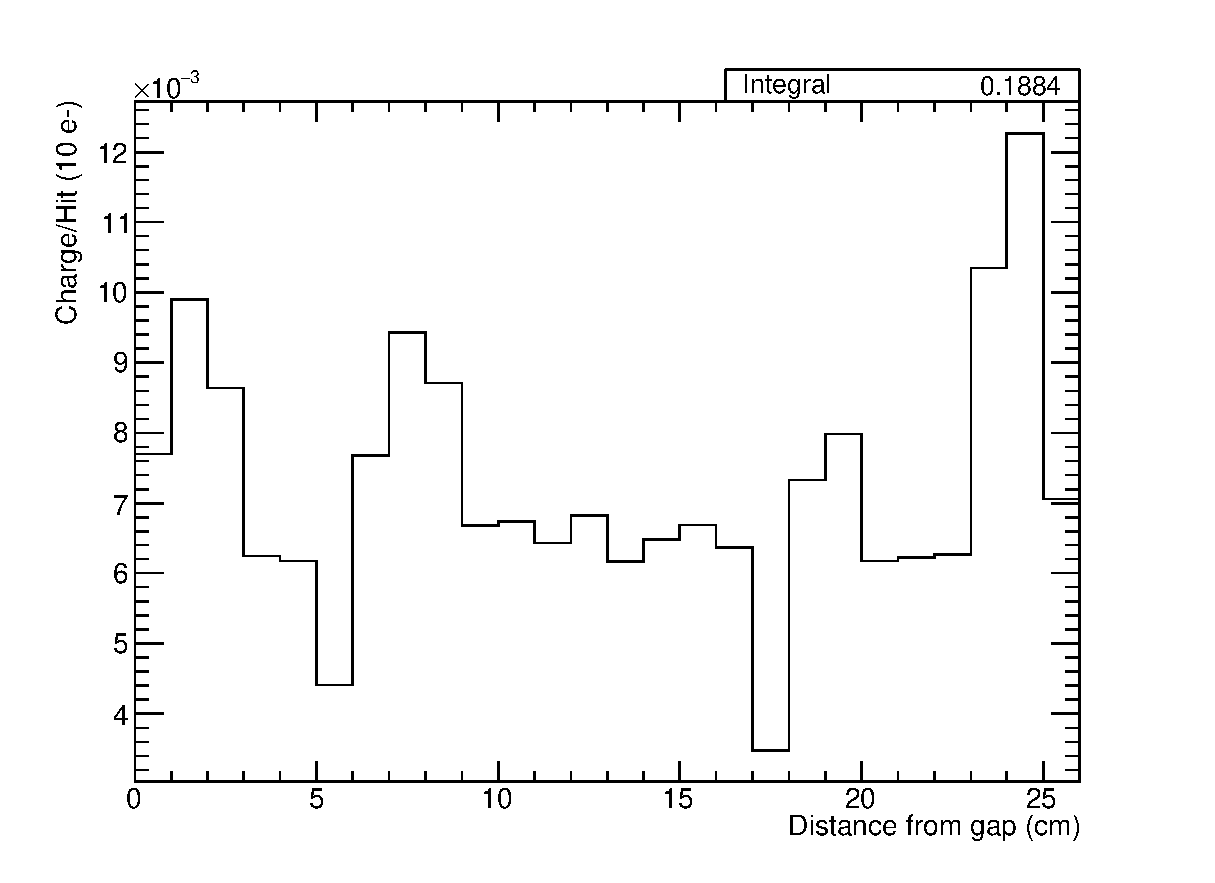
\includegraphics[width=0.98\textwidth]{ChargeHit.eps}
    \caption{Average reconstructed hit charge.}
    \label{fig:HitGapDistanceCharge}
  \end{subfigure}
  \caption[The number of hits, and the average reconstructed hit charge, as a function of distance of the collection point from the nearest APA gap.]{The number of hits, and the average reconstructed hit charge, as a function of distance of the collection point from the nearest APA gap.}
  \label{fig:HitGapDistance}
\end{figure}

\begin{figure}
  \centering
  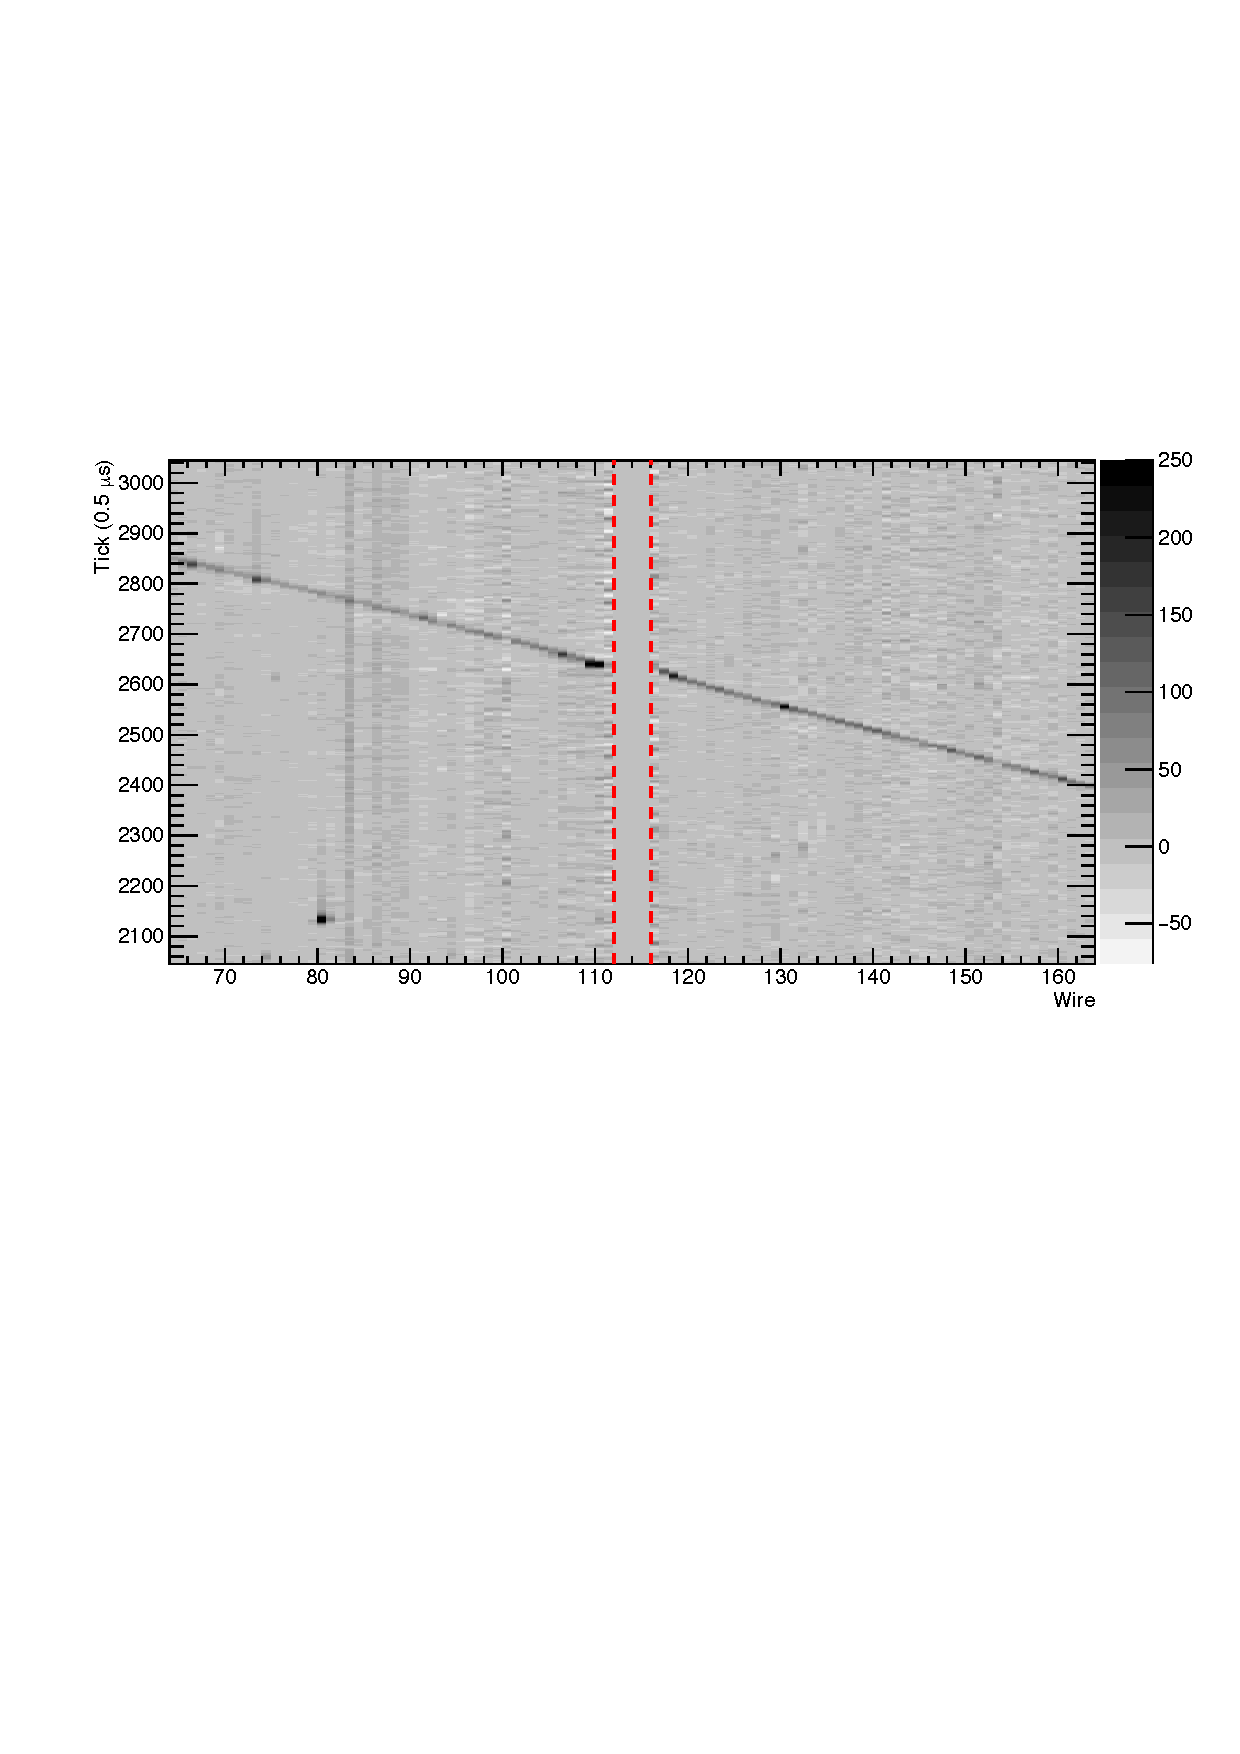
\includegraphics[width=12cm]{evd_gap.pdf}
  \caption[Event display of an APA gap-crossing track, focussed on the gap region.]{Event display of an APA gap-crossing track, focussed on the gap region.  Charge arriving at the centre of a gap deflects toward the nearest wire and is collected at a slightly later time.  This results in more charge being deposited on wires nearest the gap, with a larger spread in time.  This is subtly observable in the charge distributions shown here.}
  \label{fig:evd_gap}
\end{figure}

%----------------------------------------------------------------------------------------------------------------------------------------------------------------------------
\section{APA-Crossing Muons}\label{sec:APACrossing}

The 35-ton is the only proposed experiment before the full DUNE far detector modules that has fully implemented anode planes within the cryostat reading out data from multiple drift regions simultaneously (ProtoDUNE will have wrapped wire APAs but will only read out one drift region each and SBND has the CPAs in the centre of the cryostat with the APAs at the edges).  Referring to Figure~\ref{fig:DUNEFarDetectorDesign}, this is a design consideration that features prominently in the eventual detector so any implications in the data must be well understood.  Analysis of tracks which pass through the APAs and deposit charge in both drift regions is the subject of this section.

In Section~\ref{sec:APACrossingT0}, a method to determine the absolute event time, T0, from APA-crossing tracks is presented and in Section~\ref{sec:APACrossingCharge} the charge deposited by these tracks, particularly when crossing through the planes, is studied.  Comparisons between the two drift regions, made possible by comparing tracks left by the same particle, are contained in Section~\ref{sec:APACrossingDriftComparison}.

%----------------------------------------------------------------------------------------------------------------------------------------------------------------------------
\subsection{T0 Determination from APA Crossing Tracks}\label{sec:APACrossingT0}

Given the nature of a TPC detector, an `event time' (T0) must be known in order to set an absolute timescale, and therefore absolute position, on all interactions within the detector.  An accurate T0 is essential for calorimetric reconstruction: in order to understand how much charge a hit had when it was created, a lifetime correction dependent on the total drift time must be applied.  An incorrect T0 would lead to a systematic under- or over-estimation of the reconstructed energy and have implications in particle identification and shower energy determination.

In a LArTPC, an event time is usually given by an external triggering system.  The DUNE far detector will rely on the instantaneous detection of photons produced from the immediate recombination of the ionisation electrons with positive Ar ions.  In the 35-ton, an additional external system was provided by the scintillation counters.  Since the sample of APA-crossing muons used in this analysis were all selected and reconstructed using counter information, an interaction time is immediately known.

Without correctly accounting for T0, the tracks on each side of the APAs appear offset from the planes.  This is evident from the event display shown in Figure~\ref{fig:evd_crossing}.  By aligning the track segments on either side of the APAs, a measurement of T0 can be made directly from the TPC data.

%----------------------------------------------------------------------------------------------------------------------------------------------------------------------------
\subsubsection{Aligning APA Crossing Tracks}\label{sec:APACrossingAlignment}

Two complementary methods were used to accurately align the track segments across the APA.  Both involved initially correcting for the counter T0, $T_0^{\mathrm{counter}}$, before considering a range of alternative T0 hypotheses and minimising a relevant metric to determine the most likely value.  In the first method, demonstrated in Figure~\ref{fig:APACrossingAlignmentLeastSq}, a least square linear fit is applied to the track and the residual minimised (the `residual method').  The second method, demonstrated in Figure~\ref{fig:APACrossingAlignmentSeparation}, involves fitting a line to each segment in turn and minimising the projected distance between the intersections of the lines with the centre of the APAs ($x=0$) (the `separation point method').  As will be shown, and can be seen from Figures~\ref{fig:APACrossingAlignmentLeastSqMin} and~\ref{fig:APACrossingAlignmentSeparationMin}, the two methods agree very well with each other.

\begin{figure}
  \centering
  \begin{subfigure}[t]{0.48\linewidth}
    \centering
    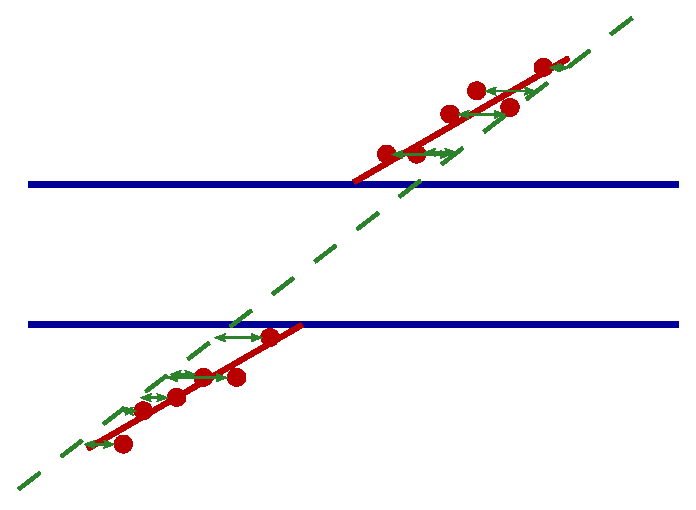
\includegraphics[width=\textwidth]{track_residual.eps}
    \caption{Demonstration of the calculation of residuals from a linear fit through all hits.  The red points are hits and the green line represents a linear fit through all points on both sides of the APA.}
    \label{fig:APACrossingAligmentLeastSqResidual}
  \end{subfigure}
  \hfill
  \begin{subfigure}[t]{0.48\linewidth}
    \centering
    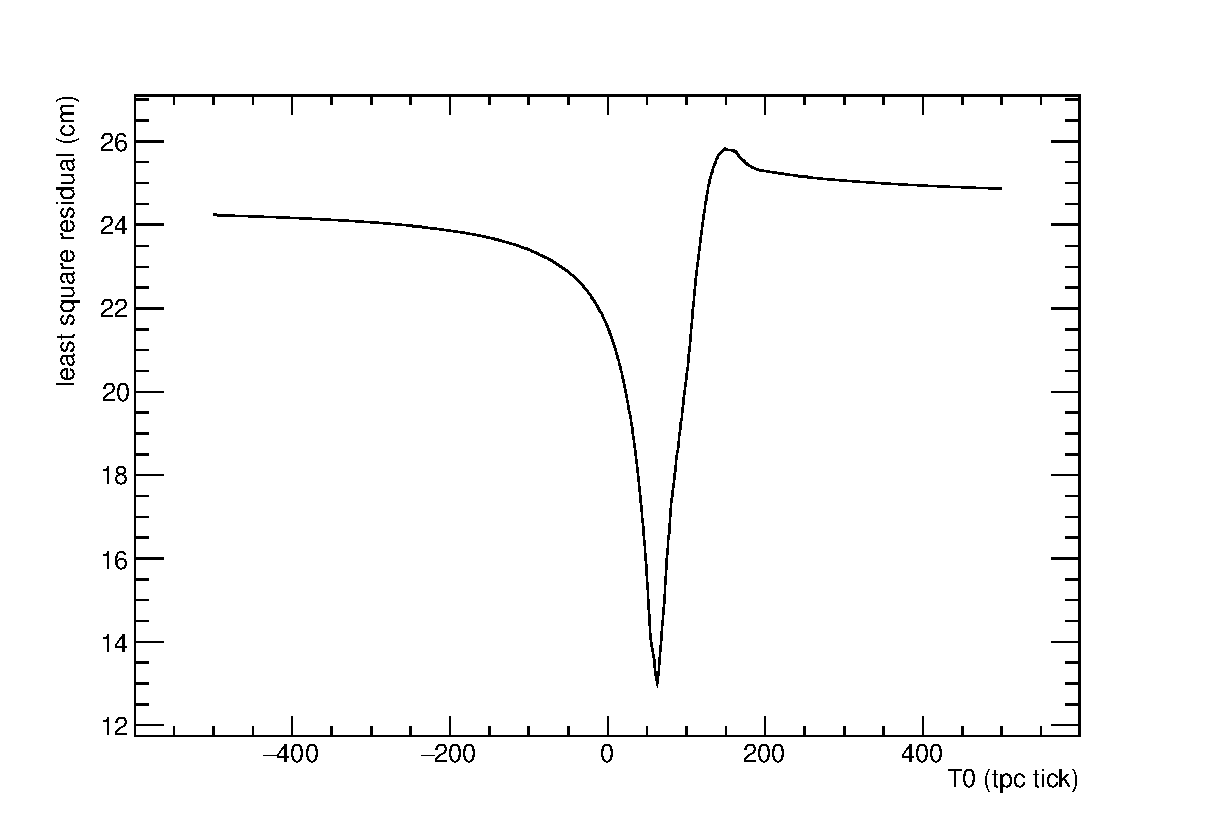
\includegraphics[width=\textwidth]{chisquare.eps}
    \caption{The residuals to the linear fit of the track over a range of T0 candidates.  The value of T0 which minimises this distribution (62 ticks in this case) is considered the most likely interaction time.}
    \label{fig:APACrossingAlignmentLeastSqMin}
  \end{subfigure}
  \caption[Method to align track segments on either side of the APAs involving minimising residuals from linear least square fit.]{Method to align track segments on either side of the APAs involving minimising residuals from a linear least square fit.  A fit is applied to all hits and the resulting residual, a representation of the `goodness of fit', is minimised over a range of T0 candidates to find the most likely interaction time for the particle leaving the track.}
  \label{fig:APACrossingAlignmentLeastSq}

  \vspace*{\floatsep}

  \begin{subfigure}[t]{0.48\linewidth}
    \centering
    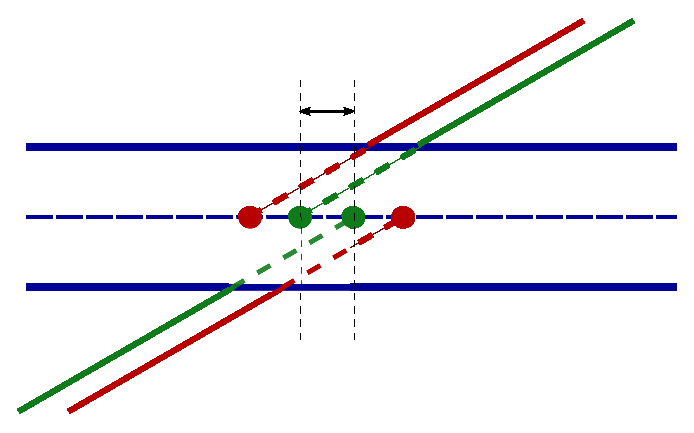
\includegraphics[width=\textwidth]{track_separation.eps}
    \caption{Demonstration of the determination of the distance between the track segments at the centre of the APAs.  The red and green lines represent linear fits to the hits (applied separately on each side of the APA) for different values of T0.}
    \label{fig:APACrossingAligmentLeastSqSeparation}
  \end{subfigure}
  \hfill
  \begin{subfigure}[t]{0.48\linewidth}
    \centering
    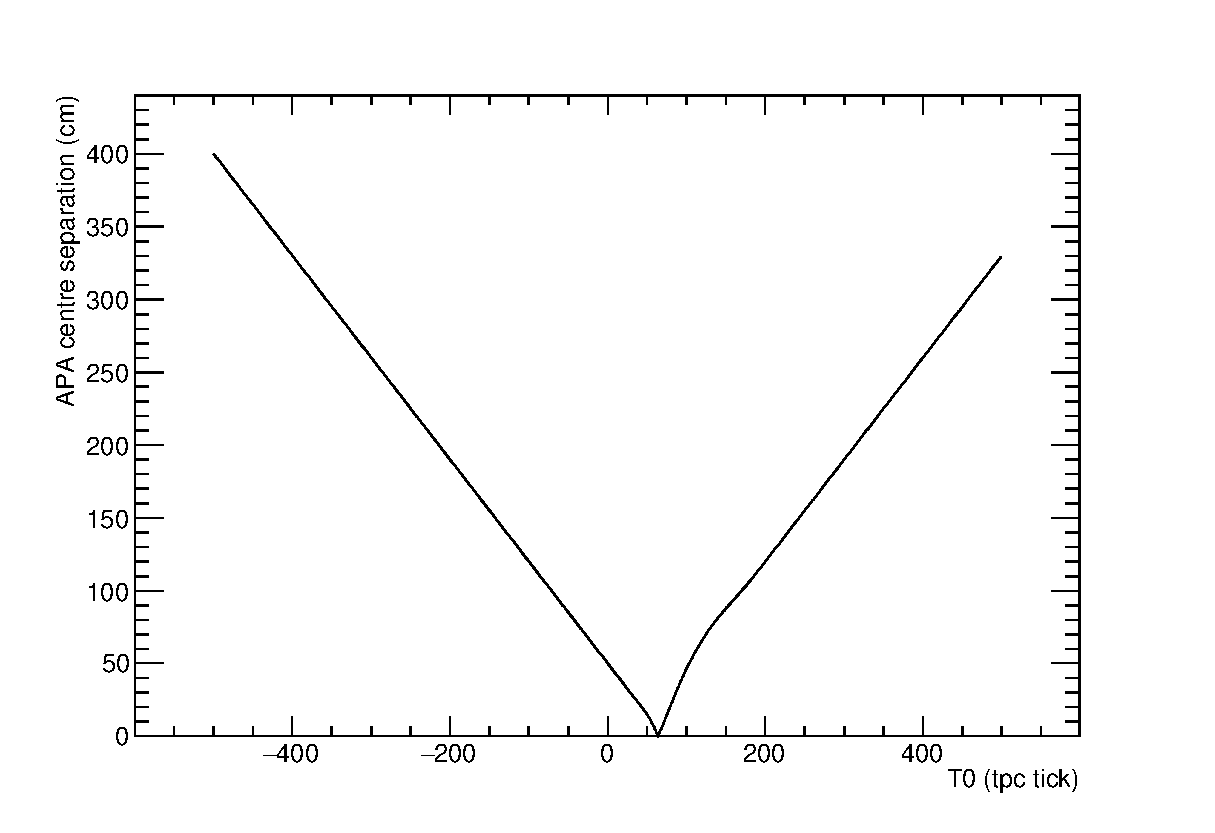
\includegraphics[width=\textwidth]{separation.eps}
    \caption{The separation distance over a range of T0 candidates.  The value of T0 which minimises this distribution (63 ticks in this case) is considered the most likely interaction time.}
    \label{fig:APACrossingAlignmentSeparationMin}
  \end{subfigure}
  \caption[Method to align track segments on either side of the APAs involving minimising the distance between the projected intersection of each with the centre of the APAs.]{Method to align track segments on either side of the APAs involving minimising the distance between the projected intersection of each with the centre of the APAs.  A fit is applied to each track segment separately and the distance between the intersection of these lines with the centre of the APA is minimised over a range of T0 candidates to find the most likely interaction time for the particle leaving the track.}
  \label{fig:APACrossingAlignmentSeparation}
\end{figure}

Naively, one would expect the T0 determined using these methods, $T_0^{\mathrm{TPC}}$, to agree with $T_0^{\mathrm{counter}}$.  This is confirmed by applying the analysis to simulated data and demonstrated in Figure~\ref{fig:TPCCounterT0DifferenceMC}.  However, there appears to be a systematic offset between the T0 given by the counters and measured from the TPC data in the 35-ton.  The distribution of this discrepancy is shown in Figures~\ref{fig:TPCCounterT0DifferenceData} and~\ref{fig:TPCCounterT0DifferenceDataResidual} for each of the two methods described; it peaks around 61 ticks (30.5~$\mu$s) and is importantly incompatible with zero.  This suggests an inconsistency somewhere in the data taking and attempts to understand this track misalignment will be the subject of the remainder of this section.  Figure~\ref{fig:TPCCounterT0Correction} shows an example track before and after this disparity is corrected for.  As is evident from Figure~\ref{fig:TPCCounterT0Difference}, the separation point method provides more consistent results so this will be used exclusively for alignment measurements in the rest of this section.

\begin{figure}
  \centering
  \begin{subfigure}[t]{\linewidth}
    \centering
    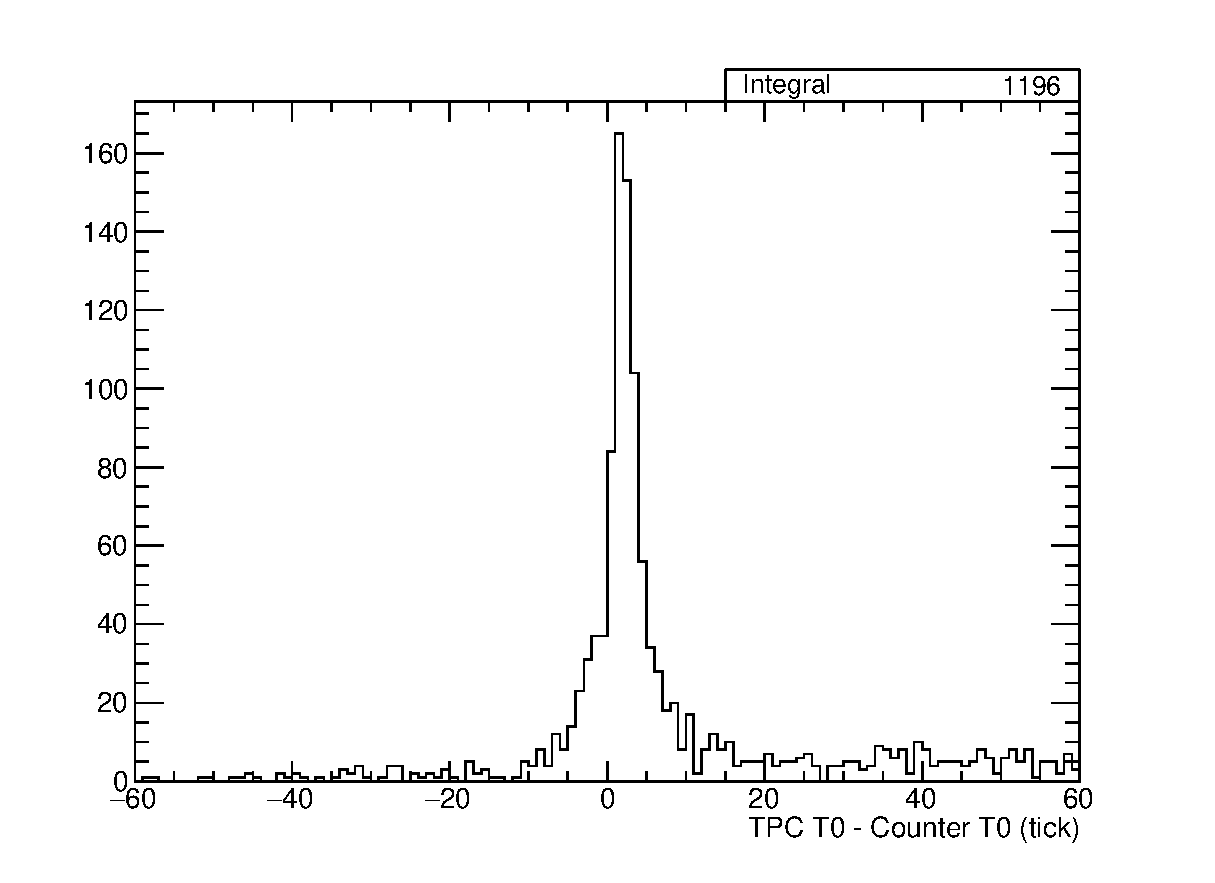
\includegraphics[width=0.51\textwidth]{TPCCounterT0DifferenceMC.eps}
    \caption{35-ton simulation.  The difference in the two measurements of T0 is distributed around zero, as expected, and validates the method.  The peak is actually at 1~tick, indicating a slight systematic offset.}
    \label{fig:TPCCounterT0DifferenceMC}
  \end{subfigure}
  \vfill
  \begin{subfigure}[t]{0.48\linewidth}
    \centering
    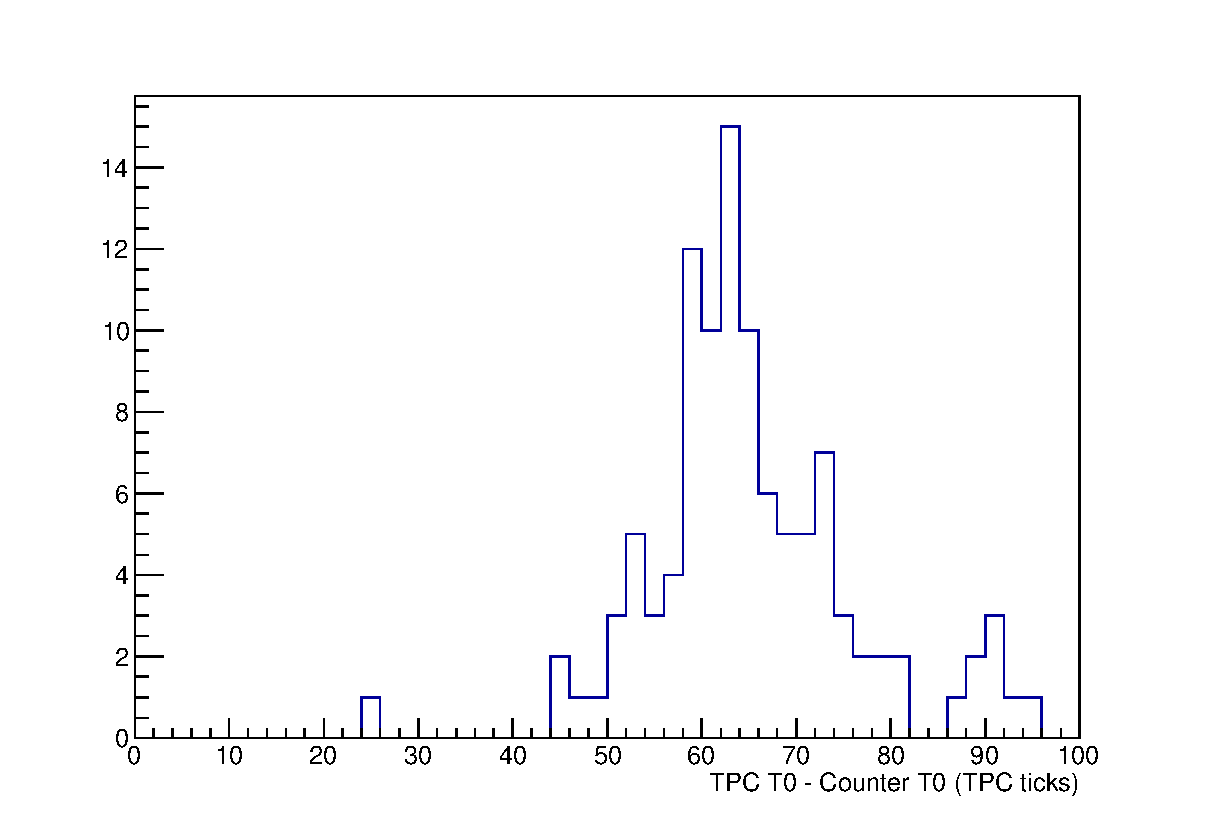
\includegraphics[width=0.98\textwidth]{TPCCounterT0DifferenceData.eps}
    \caption{35-ton data using the separation point method.}
    \label{fig:TPCCounterT0DifferenceData}
  \end{subfigure}
  \hfill
  \begin{subfigure}[t]{0.48\linewidth}
    \centering
    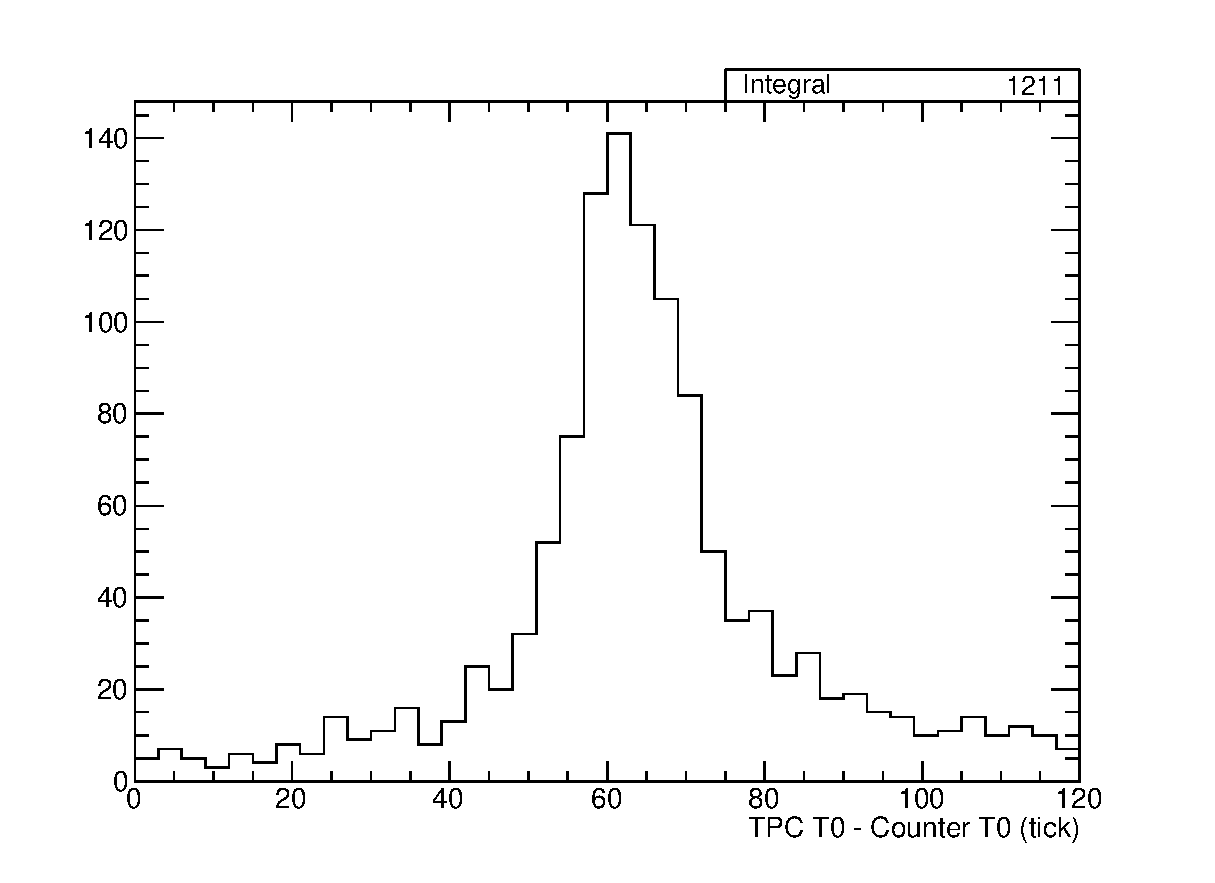
\includegraphics[width=0.98\textwidth]{TPCCounterT0DifferenceDataResidual.eps}
    \caption{35-ton data using the residual method.}
    \label{fig:TPCCounterT0DifferenceDataResidual}
  \end{subfigure}
  \caption[Difference between the T0 calculated from TPC data and the T0 provided by the counters representing the trigger time of the through-going muon, for simulation and data.]{Difference between the T0 calculated from TPC data and the T0 provided by the counters representing the trigger time of the through-going muon, for simulation (Figure~\ref{fig:TPCCounterT0DifferenceMC}) and data (Figures~\ref{fig:TPCCounterT0DifferenceData} and~\ref{fig:TPCCounterT0DifferenceDataResidual}).  If the two measurements of T0 agree the distribution would peak around zero, confirmed in simulation; the fact this is not the case for data is indicative of a systematic offset somewhere in the data taking.}
  \label{fig:TPCCounterT0Difference}
\end{figure}

\begin{figure}
  \centering
  \begin{subfigure}[t]{0.48\linewidth}
    \centering
    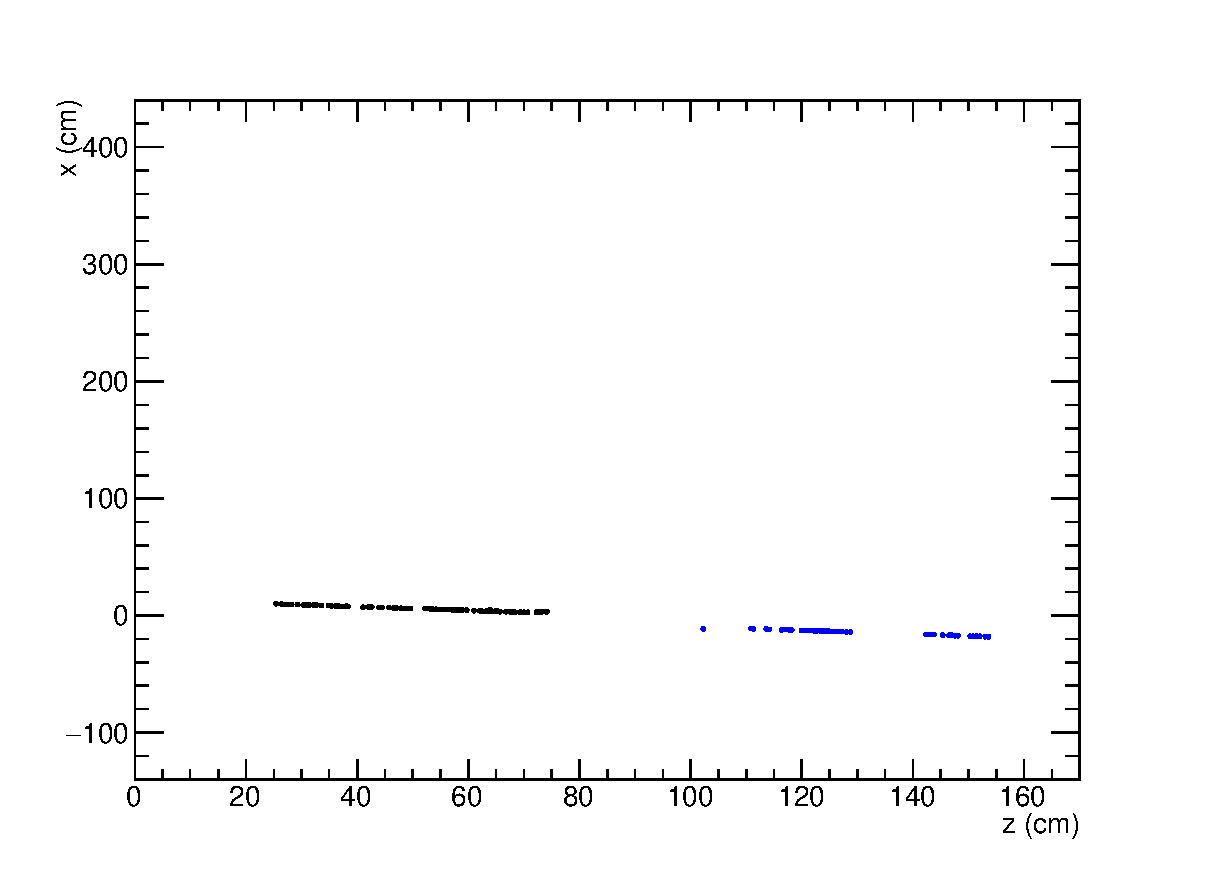
\includegraphics[width=\textwidth]{t0correction_before.eps}
    \caption{Correcting for $T_0^{\mathrm{counter}}$.}
    \label{fig:TPCCounterT0CorrectionCounter}
  \end{subfigure}
  \hfill
  \begin{subfigure}[t]{0.48\linewidth}
    \centering
    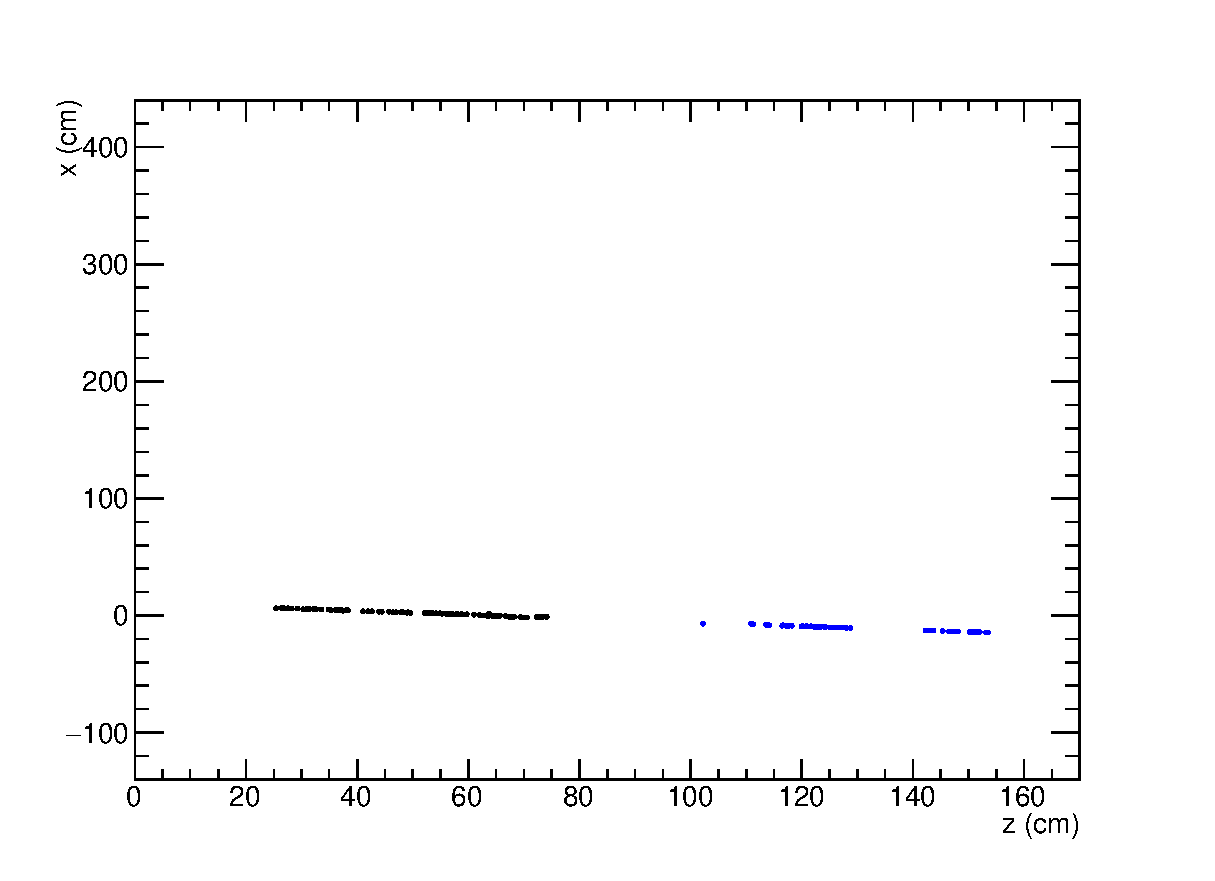
\includegraphics[width=\textwidth]{t0correction_after.eps}
    \caption{Correcting for $T_0^{\mathrm{TPC}}$.}
    \label{fig:TPCCounterT0CorrectionTPC}
  \end{subfigure}
  \caption[Correcting for T0 using $T_0^{\mathrm{counter}}$ and $T_0^{\mathrm{TPC}}$.]{Correcting for T0 using $T_0^{\mathrm{counter}}$ (Figure~\ref{fig:TPCCounterT0CorrectionCounter}) and $T_0^{\mathrm{TPC}}$ (Figure~\ref{fig:TPCCounterT0CorrectionTPC}).  The difference is subtle but noticeable; the method for determining T0 directly from the TPC data can be validated by eye.  The minimisation of the metrics to determine $T_0^{\mathrm{TPC}}$ in this case are demonstrated in Figs. \ref{fig:APACrossingAlignmentLeastSqMin} and \ref{fig:APACrossingAlignmentSeparationMin}.}
  \label{fig:TPCCounterT0Correction}
\end{figure}

%Attempts to understand the misalignment of the tracks across the APAs are presented in the remainder of this section.
%% the inconsistency between $T_0^{\mathrm{counter}}$ and $T_0^{\mathrm{TPC}}$ are presented in the remainder of this section.

%----------------------------------------------------------------------------------------------------------------------------------------------------------------------------
\subsubsection{Understanding the Misalignment of APA-Crossing Tracks}\label{sec:APACrossingMisalignment}

The underlying issue described above is essentially a misalignment of the same particle track between the two drift regions, demonstrated plainly in Figure~\ref{fig:TrackMisalignment}.  This obviously implies a misunderstanding somewhere in the data processing and stems from an issue with the detector or data readout.  The most obvious cause is a miscalibration of the DAQ timing systems for the separate detector components, as previously assumed.  There are however other possible solutions to the problem, and it is likely the effect arises from a combination of different factors.

\begin{figure}
  \centering
  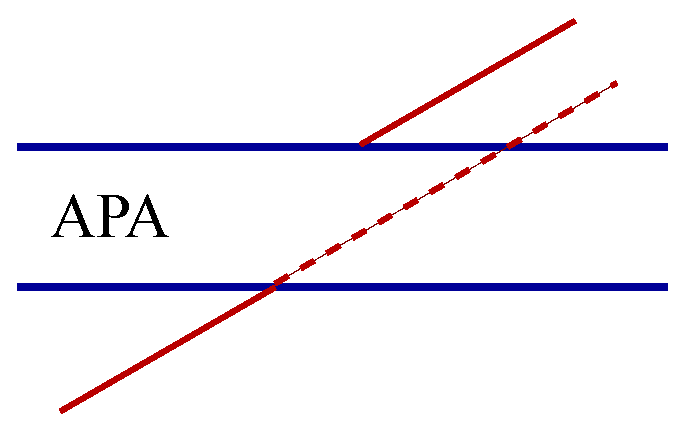
\includegraphics[width=8cm]{misalign_track_geo.eps}
  \caption[Demonstration of the effect observed in the 35-ton data concerning tracks crossing the APAs.]{Demonstration of the effect observed in the 35-ton data concerning tracks crossing the APAs.  Even after correcting for the T0 provided by the counters, there is still a misalignment of the track segments across the APA frames.}
  \label{fig:TrackMisalignment}
\end{figure}

\paragraph{Geometry}

Apart from timing, a misunderstanding of the geometry could explain this perceived misalignment.  The spacing between the collection planes is one such example, as demonstrated in Figure~\ref{fig:TrackMisalignmentCollectionSpacingGeo}; the spacing necessary to explain this effect, determined by aligning the tracks using the methods discussed above over a range of collection plane spacing hypotheses, is demonstrated in Figure~\ref{fig:TrackMisalignmentCollectionSpacingRes}.  As is evident from the figure, the collection planes must be repositioned in such a way that they would be reversed; the track alignment complications cannot be explained solely by this.

\begin{figure}
  \centering
  \begin{subfigure}[t]{0.48\linewidth}
    \centering
    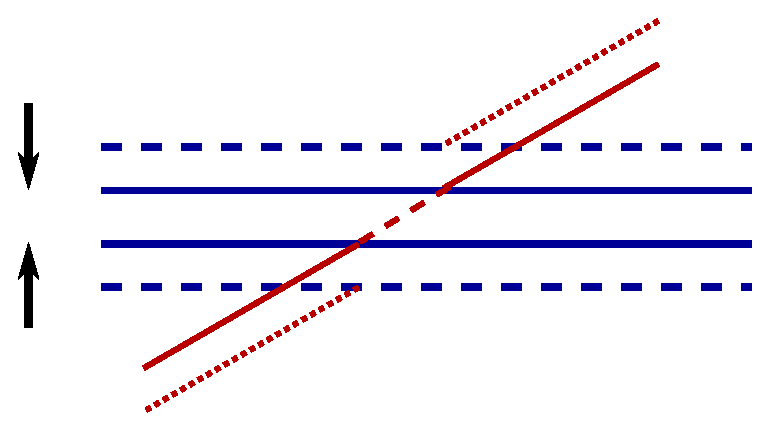
\includegraphics[width=\textwidth]{misalign_track_collection_geo.eps}
    \caption{Demonstration of how the track misalignment could be explained by an incorrect collection plane spacing.}
    \label{fig:TrackMisalignmentCollectionSpacingGeo}
  \end{subfigure}
  \hfill
  \begin{subfigure}[t]{0.48\linewidth}
    \centering
    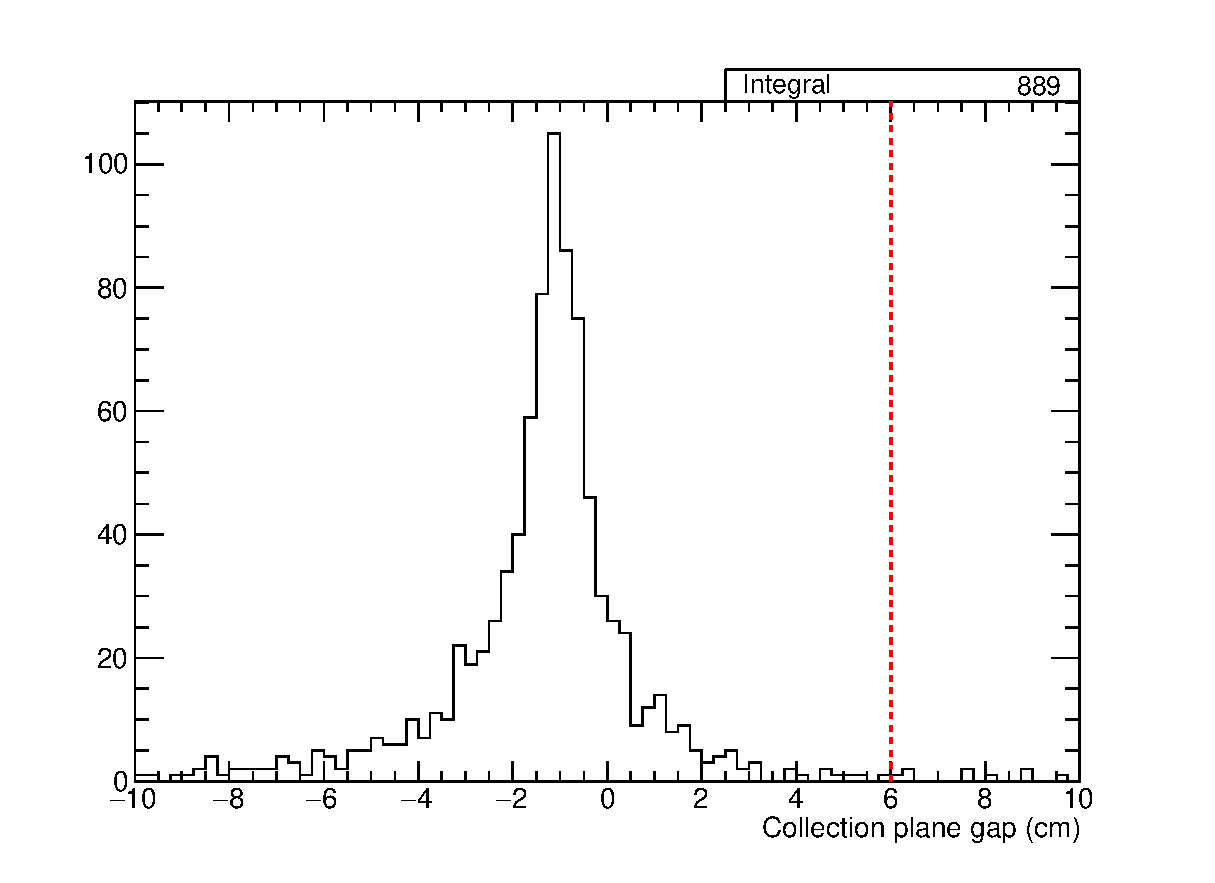
\includegraphics[width=\textwidth]{misalign_track_collection_res.eps}
    \caption{Corrected spacing between the collection planes after considering a range of values and aligning the track segments.  The red line shows the spacing used in the geometry.  The distribution peaks at $-1.19\pm0.05$~cm.}
    \label{fig:TrackMisalignmentCollectionSpacingRes}
  \end{subfigure}
  \caption[Attempting to correct the track segment misalignment by assuming a misunderstanding of the spacing between the collection planes.]{Attempting to correct the track segment misalignment by assuming a misunderstanding of the spacing between the collection planes.  It appears the resulting spacing necessary to correct for this issue would involve physically reversing the order of the planes.}
  \label{fig:TrackMisalignmentCollectionSpacing}
\end{figure}

A further problem is related to the wire positioning on the APAs in the $z$-direction; it is understood there may be a discrepancy between the two sides of the APA resulting in hits from the long and short drift regions at the same $z$-position reconstructed with a systematic offset.  Figure~\ref{fig:TrackMisalignmentZPositionGeo} shows how this could be utilised to explain the apparent track misalignment with Figure~\ref{fig:TrackMisalignmentZPositionRes} showing the distribution of corrected $z$ positions necessary to resolve the issue.  Offsets of $\sim2$~cm, as suggested by these results, are highly unlikely given the scale of offsets identified in Section~\ref{sec:APAOffsetMeasurements}, indicating again the track alignment problem cannot be resolved in this way.

\begin{figure}
  \centering
  \begin{subfigure}[t]{0.48\linewidth}
    \centering
    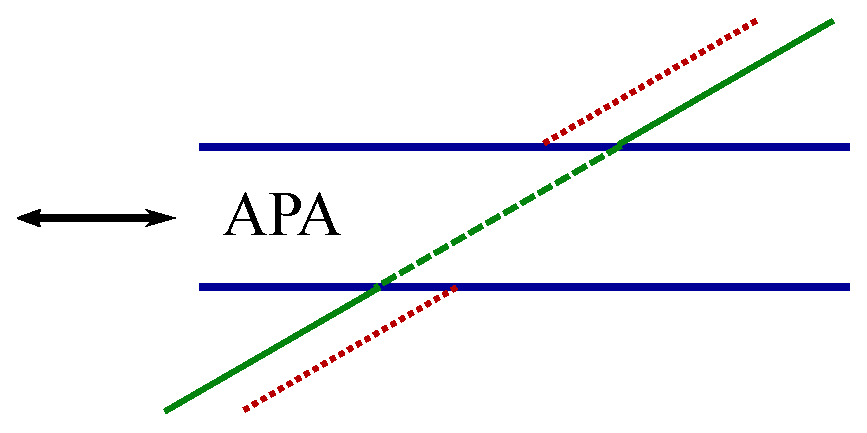
\includegraphics[width=\textwidth]{misalign_track_wire_geo.eps}
    \caption{Demonstration of how the track misalignment could be explained by an offset in the wire $z$-position on either side of the APA.}
    \label{fig:TrackMisalignmentZPositionGeo}
  \end{subfigure}
  \hfill
  \begin{subfigure}[t]{0.48\linewidth}
    \centering
    \includegraphics[width=\textwidth]{misalign_track_wire_res.eps}
    \caption{Corrected $z$-positions of the APA wires after considering a range of values and aligning the track segments.}
    \label{fig:TrackMisalignmentZPositionRes}
  \end{subfigure}
  \caption[Attempting to correct the track segment misalignment by assuming a misunderstanding of the positioning of the collection wires inside the detector.]{Attempting to correct the track segment misalignment by assuming a misunderstanding of the positioning of the collection wires inside the detector.  The wire offset would have to be around $2$~cm to fix this issue.}
  \label{fig:TrackMisalignmentZPosition}
\end{figure}

\paragraph{Drift velocity}

The drift velocity affects the angle of the tracks in wire/time space; a high velocity would result in a refraction-like effect towards the APA planes.  As demonstrated in Figure~\ref{fig:TrackMisalignmentDriftVelocityGeo}, this could explain the track segment misalignment if the effect was large enough.  Figure~\ref{fig:TrackMisalignmentDriftVelocityRes} shows the necessary drift velocity required to account for the disparity observed in data; compared to a nominal value of $109$~cm/ms, the scale of the change required to explain the oddity is unreasonably large, around a factor of five.

\begin{figure}
  \centering
  \begin{subfigure}[t]{0.48\linewidth}
    \centering
    \includegraphics[width=\textwidth]{misalign_track_drift_geo.eps}
    \caption{Demonstration of how the track misalignment could be explained by an incorrect drift velocity.}
    \label{fig:TrackMisalignmentDriftVelocityGeo}
  \end{subfigure}
  \hfill
  \begin{subfigure}[t]{0.48\linewidth}
    \centering
    \includegraphics[width=\textwidth]{misalign_track_drift_res.eps}
    \caption{Corrected drift velocity required to align the track across the APAs.  The red line shows the assumed value of 109~cm/ms.}
    \label{fig:TrackMisalignmentDriftVelocityRes}
  \end{subfigure}
  \caption[Attempting to correct the track segment misalignment by assuming an incorrect drift velocity.]{Attempting to correct the track segment misalignment by assuming an incorrect drift velocity.  In order to account for the effect noted in the data the drift velocity would have to be around five times larger than that initially calculated from models.}
  \label{fig:TrackMisalignmentDriftVelocity}
\end{figure}

This can be tested by measuring the drift velocity directly from the data.  Taking tracks which pass through opposite counter pairs (zero counter gradient) and comparing this drift distance with drift time is a trivial exercise, demonstrated in Figure. \ref{fig:DriftVelocity}.  The measured value of $110.2\pm0.4$~cm/ms agrees very well with the aforementioned value, determined theoretically, of $109$~cm/ms.  It may therefore be assumed the drift velocity is as expected and does not contribute at all to the track alignment anomaly.

\begin{figure}
  \centering
  \begin{subfigure}[t]{0.48\linewidth}
    \centering
    \includegraphics[width=\textwidth]{DistanceDriftTime.eps}
    \caption{Distribution of hit drift times for eight sets of counter pairs, assuming all tracks pass through the centres of the counters.}
    \label{fig:DistanceDriftTime}
  \end{subfigure}
  \hfill
  \begin{subfigure}[t]{0.48\linewidth}
    \centering
    \includegraphics[width=\textwidth]{DriftVelocity.eps}
    \caption{The eight points found from taking the Gaussian mean of the time distributions for each rough drift distance.}
    \label{fig:DriftVelocityGraph}
  \end{subfigure}
  \caption[Measuring the drift velocity of the ionisation electrons by taking tracks passing through opposite counter pairs and comparing the corresponding drift distance to the drift time.]{Measuring the drift velocity of the ionisation electrons by taking tracks passing through opposite counter pairs and comparing the corresponding drift distance to the drift time.  Assuming all tracks pass through the geometric centres of the counters, a poor assumption, a distribution of hit time for this drift distance can be found; this is shown in \ref{fig:DistanceDriftTime}.  Taking each counter pair separately and fitting a Gaussian to the distribution of drift times nullifies the assumptions necessary due to a lack of exact knowledge, on a track by track basis, of the exact $x$-position.  This is shown in the graph in Figure~\ref{fig:DriftVelocityGraph}.}
  \label{fig:DriftVelocity}
\end{figure}

\paragraph{Timing}

The timing offset of 32~$\mu$s, calculated in Section~\ref{sec:APACrossingAlignment}, is so large it was assumed another explanation for the track segment misalignment was likely.  However, after reviewing all possibilities it appears there must be a significant timing offset present somewhere in the data.  Further evidence for this hypothesis is presented in Figure~\ref{fig:HitTimes} which displays the T0-corrected time distribution for all hits on the APA-crossing track.  The minimum drift time these hits may have, since they pass directly through the planes, is the interaction time, T0.  As is evident from the distribution in Figure~\ref{fig:HitTimesZoom}, this is around 60~ticks (30~$\mu$s) and is again notably inconsistent with zero.  The curious spike at the interaction time motivates the work presented in Section~\ref{sec:APACrossingCharge} and will be discussed there.  Additionally, it is possible to compare the T0 provided by the counters with information from the photon detectors.  This is shown in Figure~\ref{fig:TPCPhotonT0Difference} and provides further confirmation for a timing miscalibration in the TPC readout.

\begin{figure}
  \centering
  \begin{subfigure}[t]{0.48\linewidth}
    \centering
    \includegraphics[width=\textwidth]{HitTimes.eps}
    \caption{Over the full range of drift times.  The sharp dip around 500~ticks corresponds to the maximum drift time for hits in the short drift region; beyond this only hits in the long drift region contributes to the distribution.}
    \label{fig:HitTimesRange}
  \end{subfigure}
  \hfill
  \begin{subfigure}[t]{0.48\linewidth}
    \centering
    \includegraphics[width=\textwidth]{HitTimesZoom.eps}
    \caption{Zoomed in on the interaction time.  The red line is drawn at 59.5 ticks (29.8~$\mu$s) and represents, by eye, the centre of the rising edge of the distribution.}
    \label{fig:HitTimesZoom}
  \end{subfigure}
  \caption[The T0-corrected drift time for hits on APA-crossing tracks.]{The T0-corrected drift time for hits on APA-crossing tracks.  The lower leading edge of this distribution is an indication of the interaction time, T0.}
  \label{fig:HitTimes}
\end{figure}

\begin{figure}
  \centering
  \includegraphics[width=12cm]{T0OffsetTPCPhoton.eps}
  \caption[Difference between the interaction time measured by the TPC data and that provided by photon detector information.]{Difference between the interaction time measured by the TPC data and that provided by photon detector information.  Only events with a single reconstructed flash are considered, with each assumed to have been caused by the triggering particle.  This results in very few events, but clear supporting evidence of a timing offset on the order of 60 ticks is found.}
  \label{fig:TPCPhotonT0Difference}
\end{figure}

This interesting result provoked further investigation into the notion of a timing offset between detector components, specifically the TPC and counter readout (RCEs and PTB respectively).  Confirmation of this miscalibration is displayed in Figure~\ref{fig:TPCCounterOffset} which shows the difference between the timestamps recorded by each of the subcomponents upon receiving the trigger.

\begin{figure}
  \centering
  \includegraphics[width=12cm]{PTBRCEDiffTimestamps.eps}
  \caption[The difference between the timestamps recorded by the PTB and the RCEs upon receiving a trigger.]{The difference between the timestamps recorded by the PTB and the RCEs upon receiving a trigger.  The absolute timing for the DAQ system is given, along with most experiments at FNAL, by `NO$\nu$A time': a 64~MHz clock starting on 1st January, 2010 (with one NO$\nu$A tick therefore being 15.625~ns).  The distribution peaks sharply at 1705 NO$\nu$A ticks, or 26.6~$\mu$s.}
  \label{fig:TPCCounterOffset}
\end{figure}

There are now three measurements of the timing offset with a slight disagreement between each.  This will be discussed further in Section~\ref{sec:CombinedOffsets}.

%% Within the limitations of all methods discussed, there is agreement between the T0 offset in Figure~\ref{fig:HitTimesZoom} and the timing miscalibration in Figure~\ref{fig:TPCCounterOffset}.  This does not however account for the full track segment misalignment; this represents 64~ticks (32~$\mu$s) if accounted for using timing alone, as seen in Figure~\ref{fig:TPCCounterT0Difference}.  As previously noted, the complete solution is likely a combination of different effects.  Given that drift velocity and $z$-position of wires effects are neglible, the remaining offset must be due to a slight discrepency between the actual spacing of the collection planes and what is being assumed.  With an actual T0 of 56 ticks, this collection plane spacing can be determined in the usual way by aligning tracks.  The results of this are demonstrated in Figure~\ref{fig:RemainingCollectionSpacing}.

%% \begin{figure}
%%   \centering
%%   \caption{}
%%   \label{fig:RemainingCollectionSpacing}
%% \end{figure}

%% The misalignment of the tracks, as described in Section~\ref{sec:APACrossingAlignment}, can be understood as a combination of a timing miscalibration between two detector components and a slight offset in the geometry, which is not unexpected.

%----------------------------------------------------------------------------------------------------------------------------------------------------------------------------
\subsubsection{Combined Offset Analysis}\label{sec:CombinedOffsets}

The discussion in Section~\ref{sec:APACrossingMisalignment} hints strongly at an intrinsic timing offset present in the data.  However, as already shown in Section~\ref{sec:APAGapCrossing}, it is understood there are geometrical offsets in the positions of the APAs in the $x$- and $z$-dimensions.  Attempting to measure all these offsets simultaneously presents challenges since they all affect each other.  It is possible the tension between the measurements of the timing offset may be resolved by combining the results from each of the offset calculations.

The timing offset will not influence the determination of the geometrical APA gaps (found in Section~\ref{sec:APAGapCrossing}) unless the track segments used to measure the gaps cross through the APA frames; the timing is consistent for each drift region.  A simple cut was used to exclude such events when making these measurements.  However, the geometrical offsets will have an impact on the APA crosser analysis.  For example, the drift times measured for each hit will be affected by the physical positions of the APAs.  Figure~\ref{fig:HitTimesFixed} shows the distribution of the drift times for all track hits corrected for the offsets implied by the $x$-gap measurements.  It can be seen this accounts for the disparity between the previous measurements.  It does not appear to agree completely with the offsets found between the timestamps but serves to demonstrate differences from the assumed positions of the APAs have a very sizeable effect on distributions such as these.

\begin{figure}
  \centering
  \includegraphics[width=12cm]{HitTimesFixed.eps}
  \caption[The distribution of the drift times of all hits on APA-crossing tracks after correcting for the APA offsets along the direction parallel to the drift direction.]{The distribution of the drift times of all hits on APA-crossing tracks after correcting for the APA offsets along the direction parallel to the drift direction, found in Section~\ref{sec:APAGapCrossing}.  The red line represents a T0 of 53 ticks, representing the difference observed between the trigger timestamps between the scintillation counter and TPC readout systems.  The hit time distribution appears to agree with this value to a greater extent than previously (Figure~\ref{fig:HitTimesZoom}).}
  \label{fig:HitTimesFixed}
\end{figure}

Correcting for the time offset of 53~ticks implied by the sub-component timestamp miscalibration, along with those in the $x$- and $z$-positions of the APAs, does not entirely account for the initial inconsistency observed in Figure~\ref{fig:TPCCounterT0Difference}.  A similar evaluation to that undertaken in Section~\ref{sec:APACrossingMisalignment}, namely considering the required disparities in various quantities to account for this, may be used to facilitate a complete understanding.  After correcting for the three aforementioned offsets, Figure~\ref{fig:ExtraCorrections} demonstrates the necessary misunderstandings in the collection plane spacing and the $z$-positions of the collection wires to account for the remaining discrepancy.  It seems highly likely that the offsets between the APA gaps left unresolved in the short drift region, incalculable in the 35-ton data, can account for the outstanding misalignment between the track segments.  Nothing conclusive can be extracted from Figure~\ref{fig:ExtraCorrectionWire} with regards to the values of these uncertainties since this considers differences between all short drift region TPCs and long drift region TPCs together, but implies further offsets at a similar scale to those measured in the long drift region may still be present.  With corrected APA gaps in the short drift region, it is reasonable to argue the track segment misalignment between drift regions would be completely resolved.

\begin{figure}
  \centering
  \begin{subfigure}[t]{0.48\linewidth}
    \centering
    \includegraphics[width=0.98\textwidth]{ExtraCorrectionPlaneSpacing.eps}
    \caption{Assuming a misunderstanding in the spacing between the collection planes, a value of $4.74\pm0.04$~cm is measured.  This is a difference of $1.27\pm0.04$~cm from the assumed spacing, a discrepancy which is highly unlikely.}
    \label{fig:ExtraCorrectionPlaneSpacing}
  \end{subfigure}
  \hfill
  \begin{subfigure}[t]{0.48\linewidth}
    \centering
    \includegraphics[width=0.98\textwidth]{ExtraCorrectionWire.eps}
    \caption{Assuming a misunderstanding in the alignment of the collection planes in $z$ between the two drift regions, an offset of $-0.24\pm0.03$~cm is found.  Given the scale of the corrections determined in Section~\ref{sec:APAOffsetMeasurements}, and the incapability to measure the gaps in the short drift regions, this is eminently credible.}
    \label{fig:ExtraCorrectionWire}
  \end{subfigure}
  \caption[Accounting for the extra discrepancy in track alignment after fixing for all the measured offsets by assuming a misunderstanding in the collection plane spacing and the $z$-positions of the collection wires.]{Accounting for the extra discrepancy in track alignment after fixing for all the measured offsets by assuming a misunderstanding in the collection plane spacing (Figure~\ref{fig:ExtraCorrectionPlaneSpacing}) and the $z$-positions of the collection wires (Figure~\ref{fig:ExtraCorrectionWire}).}
  \label{fig:ExtraCorrections}
\end{figure}

This is the first time tracks crossing the readout planes have been used in a LArTPC experiment and have proven to be a valuable way of calibrating inter-detector components and finding other inconsistencies in the data.  Without studying this data set, the timing offset between the TPC and the external counters would not have been discovered and all analyses would naively use the incorrect T0.  The experience in characterising the offsets in the 35-ton, in time, $x$ and $z$, will be crucial when understanding the eventual DUNE far detector.  Based on experience here, it is imperative these misunderstandings are mitigated as much as possible at the far detectors, with each module containing 150 APAs and four drift regions.

%----------------------------------------------------------------------------------------------------------------------------------------------------------------------------
\subsection{Charge Deposited by APA Crossing Tracks}\label{sec:APACrossingCharge}

The intriguing distribution of the T0-corrected hit times observed in the data, shown in Figure~\ref{fig:HitTimesRange}, hints at some aspect of the detector response that needs to be understood.  In the DUNE far detector, a large number of events will contain particles which pass through the APA frames, so characterising resulting effects is critical.  The equivalent plot for simulated data is shown in Figure~\ref{fig:HitTimesMC}.  Comparing these distributions, there is a very obvious difference around the interaction time.  It appears there is an effect present in the data, not currently being simulated, which manifests in around twice as many hits occurring at T0 on the collection planes for APA-crossing tracks.  This is described in Section~\ref{sec:InteractionTimeHits} and the phenomenon is visible on event displays presented in Section~\ref{sec:HookEVDs}.

\begin{figure}
  \centering
  \includegraphics[width=12cm]{HitTimesMC.eps}
  \caption[The T0-corrected drift time for all hits on an APA-crossing track in simulation.]{The T0-corrected drift time for all hits on an APA-crossing track in simulation.  The equivalent plot for 35-ton data is shown in Figure~\ref{fig:HitTimesRange}.}
  \label{fig:HitTimesMC}
\end{figure}

%----------------------------------------------------------------------------------------------------------------------------------------------------------------------------
\subsubsection{Interaction Time Hits}\label{sec:InteractionTimeHits}

The excess of hits at the interaction time is due to the use of a grounded `mesh' at the centre of the APAs.  The purpose of such a design choice is to ensure a uniform electric field across the face of the APA; without it the field would be ill-defined given the presence of the grounded, rectangular APA frames with positively biased planes on either side.  It is plausible therefore to consider a `backward-facing' field being set up between the grounded mesh and the positively biased collection planes which would lead to hits drifting the `wrong' way when produced in this region; APA-crossing tracks would hence leave significantly more hits on the collection plane as the other planes.  This is demonstrated schematically in Figure~\ref{fig:MeshHits}.

\begin{figure}
  \centering
  \includegraphics[width=12cm]{MeshHits.eps}
  \caption[Demonstration of the electron ionisation and hit collection for APA-crossing tracks.]{Demonstration of the ionisation and hit collection for APA-crossing tracks.  The red line represents a track passing through the anode planes, shown in black.  The grey region is the centre of the APA frame on which the grounded mesh is affixed.  The red dots correspond to the ionisation of electrons which then drift, depositing charge (black dots) on the readout wires.  The three planes shown are, from left to right, the collection plane and the two induction planes.  The biasing of each of the planes and mesh sets up field lines which all terminate on the collection wires, resulting in charge collected from before the track passes through and after.}
  \label{fig:MeshHits}
\end{figure}

A convenient way of confirming whether or not the mesh can explain this excess of hits at the interaction time is possible since one of the four APAs in the 35-ton was constructed without the mesh, precisely for this purpose.  Unfortunately, this was the APA which was most plagued by noise issues, so very little good data is available from channels on this APA.  It is however possible to make a crude comparison; this is shown in Figure~\ref{fig:HitTimesAPAs}.  This appears to confirm the sharp peak of hits occurring at the interaction time comes from the APAs which use a mesh.

\begin{figure}
  \centering
  \begin{subfigure}[t]{0.48\linewidth}
    \centering
    \includegraphics[width=\textwidth]{HitTimesAPA023.eps}
    \caption{Hit times for all hits on APAs 0, 2 and 3; these are the three APAs containing the grounded mesh at the centre.}
    \label{fig:HitTimesAPA023}
  \end{subfigure}
  \hfill
  \begin{subfigure}[t]{0.48\linewidth}
    \centering
    \includegraphics[width=\textwidth]{HitTimesAPA1.eps}
    \caption{Hit times for all hits on APA 1, the APA without a grounded mesh at its centre.}
    \label{fig:HitTimesAPA1}
  \end{subfigure}
  \caption[Comparison between the T0-corrected hit time distributions on APAs with and without the grounded mesh.]{Comparison between the T0-corrected hit time distributions on APAs with and without the grounded mesh.  Even given the very low statistics in Figure~\ref{fig:HitTimesAPA1}, there is a noticeable difference in the distribution of hits around the interaction time.}
  \label{fig:HitTimesAPAs}
\end{figure}

Using the 35-ton dataset, it is also possible to confirm that the mesh is functioning as expected.  Without a mesh, one may expect a difference between the hits deposited on wires towards the centre of an APA face and wires at the edges, in front of the grounded frame.  The functionality of the grounded mesh ensures there is no difference between any wires on a given APA.  Figure~\ref{fig:HitTimesFrame} confirms this is the case.

\begin{figure}
  \centering
  \includegraphics[width=10cm]{HitTimesFrame.eps}
  \caption[Comparison between the distribution of T0-corrected hit times for hits on wires in front of the APA frame and away from the APA frame to validate the functionality of the mesh.]{Comparison between the distribution of T0-corrected hit times for hits on wires in front of the APA frame and away from the APA frame to validate the functionality of the mesh.  Both distributions are normalised by the number of entries.  There is no evidence of any differences between the two distributions so this suggests the mesh is working as intended.}
  \label{fig:HitTimesFrame}
\end{figure}

A natural question to pose at this point is to ask if these `extra' hits deposited by APA-crossing tracks as a result of this `backwards' field have similar properties to the `correct' hits.  The most important property to consider is the charge of the hits; Figure~\ref{fig:HitCharges} shows the average charge per hit for hits occurring at the interaction time and all other hits.  It is clear from this there is nothing different about these additional hits and they can be treated in the same way.

\begin{figure}
  \centering
  \begin{subfigure}[t]{0.48\linewidth}
    \centering
    \includegraphics[width=\textwidth]{HitChargeInteraction.eps}
    \caption{Hits occurring around the interaction time; 50 < tick < 70.  A fitted Gaussian of the peak yields a mean of 149 and width of 49.}
    \label{fig:HitChargeInteraction}
  \end{subfigure}
  \hfill
  \begin{subfigure}[t]{0.48\linewidth}
    \centering
    \includegraphics[width=\textwidth]{HitChargeNonInteraction.eps}
    \caption{Hits occurring away from the interaction time; tick < 50, tick > 70.  A fitted Gaussian of the peak yields a mean of 152 and a width of 28.}
    \label{fig:HitChargeNonInteraction}
  \end{subfigure}
  \caption[Average lifetime-corrected charge per hit for hits on an APA-crossing track separated according to whether or not the hit was collected around the interaction time.]{Average lifetime-corrected charge per hit for hits on an APA-crossing track separated according to whether or not the hit was collected around the interaction time.  There is no evidence to suggest the `extra' hits collected around the interaction time have significantly more or less average charge than `regular' hits.}
  \label{fig:HitCharges}
\end{figure}

As alluded to earlier, the DUNE simulation software is simplistic and does not simulate any ionisation within the region of the APA planes; in the case of APA-crossing muons this results in no hits being created after the track passes through the first induction wires.  Evidently, this is an important region and must be understood and well simulated in order to test reconstruction and analyses.  When this is added to the software, the 35-ton data will be essential for validation purposes.

%----------------------------------------------------------------------------------------------------------------------------------------------------------------------------
\subsubsection{Event Displays of APA-Crossing Tracks}\label{sec:HookEVDs}

The effect investigated in Section~\ref{sec:InteractionTimeHits} is directly observable in the raw data, as shown in Figure~\ref{fig:EVDHook}.  The electrons ionised as the particle track passes between the collection plane and the mesh are observable as hits which appear to have drifted in the negative time direction.  The outcome is a little `hook' shape in the data.

\begin{figure}
  \centering
  \begin{subfigure}[t]{0.9\linewidth}
    \centering
    \includegraphics[width=\textwidth]{evd_hook_raw.pdf}
    \caption{Raw}
    \label{fig:EVDHookRaw}
  \end{subfigure}
  \begin{subfigure}[t]{0.9\linewidth}
    \vspace{0.5cm}
    \centering
    \includegraphics[width=\textwidth]{evd_hook_reconstructed.pdf}
    \caption{Reconstructed}
    \label{fig:EVDHookReconstructed}
  \end{subfigure}
  \caption[Event display of an APA-crossing track with the charge deposited as it passes through the APAs evident.]{Event display of an APA-crossing track with the charge deposited as it passes through the APAs evident.  Figure~\ref{fig:EVDHookRaw} shows the raw charge and Figure~\ref{fig:EVDHookReconstructed} shows the reconstructed hits.  The `hook'-like effect is visible, with hits at apparently negative drift time.  The cm scale on Figure~\ref{fig:EVDHookReconstructed} is provided as a guide and is not completely correct due to the differing fields.}
  \label{fig:EVDHook}
\end{figure}

%----------------------------------------------------------------------------------------------------------------------------------------------------------------------------
\subsection{Comparing Drift Regions with APA-Crossing Tracks}\label{sec:APACrossingDriftComparison}

APA-crossing tracks may be utilised to make unique, specific measurements of the detector, made possible since they originate from the same particle.  For example, any drift velocity differences between the drift regions may be observed and the noise levels on the collection readouts on either side of the APA can be studied and compared.

The drift velocity is given by the angle of the track in wire/time space and any difference between this velocity in the two drift regions would be noticeable in a refraction-like effect.  This is demonstrated in Figure~\ref{fig:DriftVelocityDiffGeo}.  A measure of the angle between the track segments in the different regions would therefore be a measure of the change in drift velocity; this is shown in Figure~\ref{fig:DriftVelocityDiffRes}.

\begin{figure}
  \centering
  \begin{subfigure}[t]{0.48\linewidth}
    \centering
    \includegraphics[width=\textwidth]{DriftVelocityDiffGeo.eps}
    \caption{Demonstration of how differing drift velocities between the drift regions would manifest in the data.  A refraction-like effect would result in an angle between the two track segments.}
    \label{fig:DriftVelocityDiffGeo}
  \end{subfigure}
  \hfill
  \begin{subfigure}[t]{0.48\linewidth}
    \centering
    \includegraphics[width=\textwidth]{DriftVelocityDiffRes.eps}
    \caption{The angle between the track segments on either side of the APAs.  The distribution peaks around zero, implying, as expected, the drift velocity is constant in both regions.}
    \label{fig:DriftVelocityDiffRes}
  \end{subfigure}
  \caption[Using APA-crossing tracks to confirm the drift velocity is consistent between the two drift regions.]{Using APA-crossing tracks to confirm the drift velocity is consistent between the two drift regions.}
  \label{fig:DriftVelocityDiff}
\end{figure}

The relative noise on the two collection planes can be evaluated by considering the number of hits present in the counter shadow, in each drift region, which were not reconstructed as part of the track associated with the triggering particle.  The difference between each collection plane for a given event should peak at zero if similar levels of noise were observed in each drift region; this is confirmed in Figure~\ref{fig:CollectionPlaneNoise}.

\begin{figure}
  \centering
  \includegraphics[width=10cm]{CollectionPlaneNoise.eps}
  \caption[Comparison of noise levels between the two drift regions using APA-crossing tracks.]{Comparison of noise levels between the two drift regions using APA-crossing tracks.  The number of noise hits in the counter shadow for each drift region was considered separately by neglecting all hits identified as track hits, all hits on noisy wires and all hits which have a large number of closely neighbouring hits (which could be symptomatic of unrelated particle tracks).  The difference between the number of noise hits in each peaks around zero, implying similar levels of noise.}
  \label{fig:CollectionPlaneNoise}
\end{figure}

%----------------------------------------------------------------------------------------------------------------------------------------------------------------------------
\section{Shower Reconstruction in 35-ton Data}\label{sec:ShowerData}

The developments in the reconstruction for LArSoft, discussed in Chapter \ref{chap:LArTPCReconstruction}, were originally motivated by an interest in reconstructing and analysing $\pi^0$ mesons in the 35-ton data.  Given the unfortunate eventual problems prevalent in the data, such analyses would be extremely challenging and likely impossible.  Since it is still interesting and instructive to analyse how well the reconstruction performs on a sample of real data, this will be briefly explored in the present section.

Considerations relevant when applying the reconstruction developed on simulation to data are discussed in Section~\ref{sec:DataSpecificReconstruction} before the necessary reanalysis of the calorimetry is presented in Section~\ref{sec:DataCalorimetryReconstruction}.  The algorithms are applied to a shower and a $\pi^0$ candidate found in the data in Sections~\ref{sec:DataShowerReconstruction} and~\ref{sec:DataPi0Reconstruction} respectively.

%----------------------------------------------------------------------------------------------------------------------------------------------------------------------------
\subsection{Data Specific Reconstruction}\label{sec:DataSpecificReconstruction}

The BlurredCluster and EMShower algorithms, outlined in Sections~\ref{sec:BlurredCluster} and~\ref{sec:EMShower} respectively, were applied to the data in an attempt to reconstruct particle objects.  In general, the algorithms worked out of the box and required no tuning.  Since this requires real 3D reconstruction, as opposed to the subtle techniques developed to circumvent the issues with the induction planes (described in Section~\ref{sec:ReconstructingMuonTracks}), the use of more than just the collection plane is necessitated.  Reconstruction is therefore only possible for showers with large enough signals on induction planes, following the coherent noise removal and hit disambiguation.

As showering particles are likely to have a different interaction time, T0, to the triggering muon, an unassociated method for obtaining this information is required.  In general, the photon detectors are designed for this purpose so the use of these seems natural.

Since it is highly unlikely the electronics models and detector responses used in the simulation are perfectly accurate, applying the calorimetric reconstruction to the data without modification would be inappropriate.  The relevant calorimetric constants and functions must be determined from the data; this is essential for complete reconstruction and is discussed in Section~\ref{sec:DataCalorimetryReconstruction}.

%----------------------------------------------------------------------------------------------------------------------------------------------------------------------------
\subsection{Calorimetry Reconstruction}\label{sec:DataCalorimetryReconstruction}

There are two relevant calorimetric conversions which are pertinent to shower reconstruction (both previously discussed in Section~\ref{sec:Calorimetry}): the calorimetry constant and the shower energy conversion.  The methods used to determine these for data will be discussed in this section.

It should be stressed that due to the large noise levels, accurate calorimetry will not be possible in the 35-ton data.  This may be understood by considering the distribution of charge deposited by ionising particles; typically this is sampled from a Landau distribution with a most probable value dependent on the electron drift distance (due to lifetime effects).  Since hit reconstruction tends to cut on the hit `threshold', the height of the peak above pedestal, this compromises lower energy hits populating the full charge distribution and biases the reconstruction toward higher energies.  This is demonstrated in Figure~\ref{fig:DataCalorimetryThreshold}.  As far as possible, steps to mitigate these effects have been applied in the proceeding discussion.  There will however be an inevitable bias so the following should not be treated as a full, rigorous assessment.

Calorimetric reconstruction is only attempted for the collection planes where the effects of noise are mitigated somewhat compared to the induction views.  Since the data used were taken at a drift field of 250~V/cm (half the nominal voltage), the recombination factor used must take this into account.  At 500~V/cm the value is 0.63 whilst at 250~V/cm a factor of 0.52 is used.

\begin{figure}
  \centering
  \begin{subfigure}[t]{0.32\linewidth}
    \centering
    \includegraphics[width=0.98\textwidth]{HitReconstructionBias20-40.pdf}
    \caption{20~cm -- 40~cm drift.}
    \label{fig:DataCalorimetryThreshold1}
  \end{subfigure}
  \hfill
  \begin{subfigure}[t]{0.32\linewidth}
    \centering
    \includegraphics[width=0.98\textwidth]{HitReconstructionBias80-100.pdf}
    \caption{80~cm -- 100~cm drift.}
    \label{fig:DataCalorimetryThreshold2}
  \end{subfigure}
  \hfill
  \begin{subfigure}[t]{0.32\linewidth}
    \centering
    \includegraphics[width=0.98\textwidth]{HitReconstructionBias140-160.pdf}
    \caption{140~cm -- 160~cm drift.}
    \label{fig:DataCalorimetryThreshold3}
  \end{subfigure}
  \caption[The bias in the hit selection due to a high noise level in the 35-ton data.]{The bias in the hit selection due to a high noise level in the 35-ton data \cite{Brailsford2016}.  The charge distribution for through-going muons is shown for three different displacements along the drift direction, 20~cm~$<~x<$~40~cm, 80~cm~$<~x~<$~100~cm and 140~cm~$<~x~<$~160~cm and takes the form of a Landau convoluted with a Gaussian.  The red line represents a typical hit finding threshold.  The most probable value of the distribution is close to this boundary in each of the cases, resulting in the lower charge hits being missed.  This introduces a bias towards higher charge and has implications for the reliability of calorimetry in the 35-ton data sample.}
  \label{fig:DataCalorimetryThreshold}
\end{figure}

The procedure invoked to determine the calorimetry constant is largely identical to that used in simulation: the dE/dx of a through-going mip is calculated and the constant varied until the expected distribution is obtained.  The through-going muons used in the analyses described in Sections~\ref{sec:APACrossing} and~\ref{sec:APAGapCrossing} were utilised to make these measurements.  Additional necessary information, such as the interaction time (to correct the charge for lifetime) and the track angle (to correct the dE/dx for track pitch), is provided by the counters.  In order to produce reliable results, an additional cut requiring at least 20 consecutive wires with a single hit on each was applied, with the dE/dx measurement obtained using just these hits.  The eventual dE/dx distribution is demonstrated in Figure~\ref{fig:DataCalorimetrydEdx} and implies a calorimetry constant of $7.4\times10^{-3}$ (for comparison, the value used for the collection plane in simulation is $5.4\times10^{-3}$).

\begin{figure}
  \centering
  \includegraphics[width=12cm]{dEdx.eps}
  \caption[The dE/dx distribution for mips passing through the 35-ton TPC.]{The dE/dx distribution for mips passing through the 35-ton TPC.  The calorimetry constant is chosen to ensure the peak of the distribution, which ideally follows a Landau, is around 1.8-1.9~MeV/cm.}
  \label{fig:DataCalorimetrydEdx}
\end{figure}

In simulation, truth information was used to find a general charge to energy conversion used in, for example, the determination of total shower energy.  This obviously is not possible in data so a similar technique to the calculation of the calorimetry constant described above was used.  The lifetime-corrected charge and track pitch information can be utilised to find a value of dQ/dx (ADC/cm), which may then be converted into a measure of dE/dx (MeV/cm) using the calorimetry constant previously determined.  This may in turn be used to find the total deposited energy by taking into account the distance travelled by the associated track in the collection view.   As demonstrated in Figure~\ref{fig:ShowerEnergyConversion}, there exists a linear relationship between total deposited lifetime-corrected charge and the particle energy; this is also seen in data in Figure~\ref{fig:DataShowerEnergyConversion}.  This may then be used as a conversion in shower energy reconstruction.

\begin{figure}
  \centering
  \includegraphics[width=12cm]{ChargeEnergy.eps}
  \caption[Relationship between deposited charge and energy for 35-ton data, calculated using through-going mips.]{Relationship between deposited charge and energy for 35-ton data, calculated using through-going mips.  The lower edge of the distribution follows a linear pattern and it is this which the conversion is chosen to represent.  Deviations from this linear fit observed above it are related to the fundamental issues with the 35-ton data and arise from missed charge due to the problems illustrated in Figure~\ref{fig:DataCalorimetryThreshold}.  This results in hits reconstructed with a lower charge for the implied energy deposited by the mip.  It should be noted there are no cases of extra charge deposited; this concurs with this interpretation and ensures confidence in the displayed line as the correct conversion may be assumed.  A possible way to restore linearity would be to truncate the thresholding demonstrated in Figure~\ref{fig:DataCalorimetryThreshold}.}
  \label{fig:DataShowerEnergyConversion}
\end{figure}

%----------------------------------------------------------------------------------------------------------------------------------------------------------------------------
\subsection{Shower Reconstruction}\label{sec:DataShowerReconstruction}

Using the modifications discussed in Sections~\ref{sec:DataSpecificReconstruction} and~\ref{sec:DataCalorimetryReconstruction}, the performance of the showering reconstruction on real data can be assessed by applying it to an electromagnetic shower.  The result of applying the algorithms to the famous 35-ton shower depicted in Figure~\ref{fig:FamousShower} is shown in Figure~\ref{fig:FamousShowerReconstructed}.  The calorimetric reconstruction yields a dE/dx of 1.1~MeV/cm and a total shower energy of 188~MeV.  These results appear feasible and are consistent with an electron shower, for which one would expect a dE/dx peaked around 2.1~MeV/cm; 1.1~MeV/cm is not an unreasonable value in the tail of this distribution.  Given its dE/dx and energy, the most likely origin for this particle is Compton scattering of a high-energy photon produced from bremsstrahlung radiation from the cosmic muon, or from a delta ray produced by it \cite{MicroBooNECosmics2016}.

\begin{figure}
  \centering
  \includegraphics[width=12cm]{FamousShowerReconstructed.pdf}
  \caption[Result of applying the shower reconstruction on a shower observed in the 35-ton data.]{Result of applying the shower reconstruction on a shower observed in the 35-ton data.  Each small rectangle represents a reconstructed hit and the colour associated with each corresponds to a reconstructed shower object.  The stars and dotted lines represent the reconstructed start point and direction for each shower.}
  \label{fig:FamousShowerReconstructed}
\end{figure}

The T0 for this particle was determined to be 4740~ticks from reconstructing flash information collected by the photon detectors -- this makes this shower the only fully automated reconstructed particle object in the 35-ton dataset.

%----------------------------------------------------------------------------------------------------------------------------------------------------------------------------
\subsection{$\pi^0$ Reconstruction}\label{sec:DataPi0Reconstruction}

An important calorimetric test of particle detectors involves demonstrating a reasonable reconstructed $\pi^0$ mass peak.  It was for this reason that the shower reconstruction discussed in Chapter~\ref{chap:LArTPCReconstruction} was developed.  An analysis of a $\pi^0$ candidate event is briefly considered here.

Without full reconstruction and selection, identifying candidate events is very difficult.  Such an event was observed in the online event display however and is shown in Figure~\ref{fig:DataPi0Candidate}.

\begin{figure}
  \centering
  \includegraphics[width=10cm]{evd_run16110_subrun1_event29.png}
  \caption[A candidate $\pi^0$ event observed in the online event display during the run.]{A candidate $\pi^0$ event observed in the online event display during the run.}
  \label{fig:DataPi0Candidate}
\end{figure}
Unlike the shower discussed in Section~\ref{sec:DataShowerReconstruction}, there is no associated photon detector information for this event; however, one of the candidate photons passes through the APA frames so techniques developed for the APA-crosser analysis (Section~\ref{sec:APACrossing}) may be employed to determine the relevant interaction time.  Applying the calorimetry reconstruction, the dE/dx information associated with the high energy candidate photon (the one which crosses the APAs) gives a value of 4.75~MeV/cm, entirely consistent with the expectation for a photon of a distribution centred around 4.2~MeV/cm.  The low energy candidate photon travels almost completely along the collection view direction resulting in unreliable dE/dx information.  The total energy for each shower is determined to be 161.8~MeV and 500.5~MeV with an implied invariant mass of
\begin{equation}\label{eq:DataPi0CandidateMass}
m_{\pi^0} = 156.6~\textnormal{MeV},
\end{equation}
comparable to the true $\pi^0$ mass of 135~MeV.

Without fully considering uncertainties and biases present, it is not possible to make a judgement as to the performance of the basic calorimetric reconstruction discussed in Section~\ref{sec:DataCalorimetryReconstruction} or to confirm whether or not the event displayed in Figure~\ref{fig:DataPi0Candidate} represents a $\pi^0$ decay.  However, dE/dx values of 1.1~MeV/cm and 4.75~MeV/cm for different showers appear consistent with electron and photon particles respectively and, within the limits of the analysis presented here, it is conceivable the particle with invariant reconstructed mass of 156.6~MeV is indeed a $\pi^0$.

%----------------------------------------------------------------------------------------------------------------------------------------------------------------------------
\section{35-ton Data Analysis Summary}\label{sec:35tonDataSummary}

Despite initial problems with the 35-ton, good progress has been made in analyses, specifically focussing on understanding the detector.  Techniques developed will be directly applicable to the data collected with the eventual far detector and for the commissioning and operation of ProtoDUNE.

The studies using TPC-crossing muons are highly useful in developing a better understanding of the detector and will be vital for future stages in the DUNE programme.  Indeed, both measurements of APA-crossing and APA-gap crossing muons yielded unexpected offsets, demonstrating the utility of such methods and again highlighting the need for prototyping.  Despite being unable to perform a $\pi^0$ analysis with the 35-ton data, good progress was made applying the novel reconstruction methods described in Chapter~\ref{chap:LArTPCReconstruction} to real data.  This is hugely important for the future of the DUNE experiment, along with the demonstration of automated reconstruction in the 35-ton data.

In general, the 35-ton was a successful first prototype for DUNE and lessons learned are already being carried forward to ProtoDUNE and are influencing the design of the far detector.
